\documentclass[a4paper,10pt,twoside, openright]{book}
\usepackage[english]{babel}
%\usepackage[utf8]{inputenc}
\usepackage{indentfirst}
\usepackage{graphicx}
\usepackage{epigraph}
\usepackage{atlasphysics}
\usepackage{subfigure}
\usepackage{lineno}
\usepackage{setspace}
\newcommand{\AC}{\ensuremath{\text{A}_{\text{C}}}}
\newcommand{\formatGenerator}[1]{\textsc{#1}}
\newcommand{\mcnlo}{\formatGenerator{mc@nlo}}
\newcommand{\wjets}{\ensuremath{W+\mathrm{jets}}}
\providecommand{\abs}[1]{\lvert#1\rvert}
\newcommand{\dy}{\ensuremath{\Delta{}\abs{y}}}
\newcommand{\deta}{\ensuremath{\Delta{}\abs{\eta}}}
\newcommand{\mtt}{\ensuremath{m_{\ttbar{}}}}
\newcommand{\Nupup}{\ensuremath{N(\uparrow\uparrow)}}
\newcommand{\Ndodo}{\ensuremath{N(\downarrow\downarrow)}}
\newcommand{\Nupdo}{\ensuremath{N(\uparrow\downarrow)}}
\newcommand{\Ndoup}{\ensuremath{N(\downarrow\uparrow)}}


\newcommand\myskip{\vspace{\baselineskip}}
\def\Xbar{\ensuremath{\bar{X}}}
\def\XXbar{\antibar{X}}
\def\Ybar{\ensuremath{\bar{Y}}}
\def\YYbar{\antibar{Y}}
\def\Tbar{\ensuremath{\bar{T}}}
\def\TTbar{\antibar{T}}
\def\Bbar{\ensuremath{\bar{B}}}
\def\BBbar{\antibar{B}}
\newcommand\TT{\ensuremath{T\bar{T}}}
\newcommand\BB{\ensuremath{B\bar{B}}}
\newcommand\T{\ensuremath{T}}
\newcommand\B{\ensuremath{B}}
\newcommand{\TB}{\ensuremath{(T \, B)}}
\newcommand{\XT}{\ensuremath{(X \, T)}}
\newcommand{\BY}{\ensuremath{(B \, Y)}}
\def\Tlr{\ensuremath{T_{L,R}}}
\def\Blr{\ensuremath{B_{L,R}}}
\def\Ylr{\ensuremath{Y_{L,R}}}
\def\Xlr{\ensuremath{X_{L,R}}}
\def\TBlr{\ensuremath{\TB_{L,R}}}
\def\BYlr{\ensuremath{\BY_{L,R}}}
\def\XTlr{\ensuremath{\XT_{L,R}}}
\def\vlt{vector-like top partner}
\def\vlb{vector-like bottom partner}

%%%%%%%%%%%%%%%%%%%%%%%%
%%% LAZYNESS-DRIVEN DEFS
%%%%%%%%%%%%%%%%%%%%%%%%
\def\cme{center-of-mass energy}
\def\cmm2{cm$^{-2}$}
\def\sm1{s$^{-1}$}
\def\chisq{$\chi^2$}
\def\loose{{\sc Loose}}
\def\tight{{\sc Tight}}
\def\whad{\ensuremath{W_{\rm had}}}
\def\wlep{\ensuremath{W_{\rm lep}}}
\def\wi{$W_{\rm had}^{\rm type\;I}$}
\def\wii{$W_{\rm had}^{\rm type\;II}$}
\def\mreco{\ensuremath{m_{\rm reco}}}
\def\chii{{\sc ``{\small 2 \btag ged jets}''}}
\def\chiii{{\sc ``{\small 3 \btag ged jets}''}}
\def\chiv{{\sc ``{\small{\footnotesize$\geq$}4 \btag ged jets}''}}

\def\dr{\ensuremath{\Delta R}}
\def\OR{\texttt{OR}}
\def\AND{\texttt{AND}}
%\def\bjet{$b$jet}
\def\bjet{$b$-jet}
%\def\cjet{$c$jet}
\def\cjet{$c$-jet}
\def\ljet{light-jet}
\def\btag{$b$-tag}
\def\ctag{$c$-tag}
\def\mt{\ensuremath{m_T}}
\def\mtw{\ensuremath{m_T(W)}}
\def\wbx{\ensuremath{\TTbar\to Wb+X}}
\def\htx{\ensuremath{\TTbar\to Ht+X}}
\def\nontt{non-$t\bar{t}$}
\def\mclimit{\texttt{MCLimit}}
\def\cls#1{\ensuremath{CL_{\rm #1}}}
\def\hthad{\ensuremath{H_T^{\rm had}}}
\def\htfj{\ensuremath{H_T^{4j}}}
\def\tthf{\ttbar+HF}
\def\ttlf{\ttbar+light}

\def\bra#1{\mathinner{\langle{#1}|}}
\def\ket#1{\mathinner{|{#1}\rangle}}
\def\braket#1{\mathinner{\langle{#1}\rangle}}
\def\Bra#1{\left<#1\right|}
\def\Ket#1{\left|#1\right>} 
\newcommand{\Overline}[2][1]{%
  {}\mkern#1mu \overline{\mkern-#1mu #2 \mkern-#1mu}\mkern#1mu {}} 
\DeclareMathAlphabet{\mathpzc}{OT1}{pzc}{m}{it}


\linespread{1.2}                        %comando per impostare l'interlinea


%\usepackage{ulem} %sostituisce l'effetto sottolineatura all'effetto corsivo nel comando \emph{} e risolve il problema delle righe che non si spezzano

\usepackage{multirow}
\usepackage{enumerate}

\usepackage[hdivide={3cm, *, 3cm}, vscale=0.75, bindingoffset=1cm]{geometry}
\usepackage{chngpage}

\usepackage[margin=7pt,font=small,labelfont=bf]{caption}
%\usepackage[margin=10pt,font=small,labelfont=bf]{caption}
%\usepackage[format=hang,indention=-2cm,labelfont=bf]{caption}%per delle caption più carine
\usepackage{booktabs}
\usepackage{longtable}
%\usepackage{pdflscape} 
%\usepackage[pdftex]{lscape}
\usepackage{lscape}
\usepackage{slashed}

\usepackage{listings}
\lstset{language=C}

\hyphenation{ca-lo-ri-me-ter ca-lo-ri-me-ters}%serve per la sillabazione: tra parentesi 

\setlength{\headheight}{15pt}
\usepackage{pict2e}
%\usepackage{guit}

%\usepackage{natbib}
%\bibliographystyle{unsrt}
%\usepackage[babel]{csquotes}
%\usepackage[style=numeric,sorting=none]{biblatex}
%\bibliography{biblio}


%MATHS
\usepackage{amssymb}
\usepackage{amsmath}
\usepackage{latexsym}
\usepackage{amsthm}
 \newcommand{\sgn}{\mathop{\mathrm{sgn}}}
\usepackage{slashed}
\usepackage[usenames,dvipsnames,svgnames,table]{xcolor}

%\usepackage[T1]{fontenc}
%\usepackage{microtype}

\usepackage{fancyhdr}
\pagestyle{fancy}

\usepackage{eso-pic}

\usepackage{url}
\usepackage[ps2pdf,bookmarks=true,bookmarksnumbered=false,% true means bookmarks in left window are numbered
bookmarksopen=false, % true means only level 1 are displayed.
colorlinks=true,linkcolor=webred]{hyperref}
%\usepackage[pdfborder={0 0 0 0}]{hyperref}
\definecolor{webgreen}{rgb}{0, 0.5, 0} % less intense green
\definecolor{webblue}{rgb}{0, 0, 0.5} % less intense blue
\definecolor{webred}{rgb}{0.5, 0, 0} % less intense red

%END OF PACKAGES

%per includere il frontespizio (ottenuto in pdf a parte)
\newcommand\BackgroundPic{
\put(0,0){
\parbox[b][\paperheight]{\paperwidth}{%
\vfill
\centering

\includegraphics[width=\paperwidth,height=\paperheight,
keepaspectratio]{smallstuff/frontespizio}%
\vfill
}}}



%per avere l'indice senza numeri di pagina
\makeatletter 
 \newcommand{\cleantableofcontents}{% 
   \clearpage\begingroup 
   \let\ps@plain\ps@empty\pagestyle{empty}% 
   \tableofcontents\clearpage\endgroup} 
 \makeatother

%per lo stile dei capitoli
\makeatletter
\def\thickhrulefill{\leavevmode \leaders \hrule height 1ex \hfill \kern \z@}
%chstyle
\def\@makechapterhead#1{%
  \vspace*{10\p@}%
  {\parindent \z@ 
    {\raggedleft \reset@font
      \scshape \@chapapp{} \thechapter\par\nobreak}%
    \par\nobreak
    \vspace*{30\p@}
    \interlinepenalty\@M
    {\begin{spacing}{1.1} \raggedright \huge \bfseries #1\end{spacing}}%
    %{\doublespacing \raggedright \huge \bfseries #1}%
    \par\nobreak
    \hrulefill
    \par\nobreak
    \vskip 90\p@
  }}
\def\@makeschapterhead#1{%
  \vspace*{10\p@}%
  {\parindent \z@ 
    {\raggedleft \reset@font
      \scshape \vphantom{\@chapapp{} \thechapter}\par\nobreak}%
    \par\nobreak
    \vspace*{30\p@}
    \interlinepenalty\@M
    {\begin{spacing}{1.1} \raggedright \huge \bfseries #1\end{spacing}}%
    \par\nobreak
    \hrulefill
    \par\nobreak
    \vskip 90\p@
  }}



\renewcommand{\chaptermark}[1]{\markboth{\thechapter. \ #1}{}}
\renewcommand{\sectionmark}[1]{\markright{\thesection.\ #1}}
\fancyhf{}
\fancyhead[LO]{\small \nouppercase{\rightmark}}
\fancyhead[RE]{\small \nouppercase{\leftmark}}
\fancyhead[RO , LE]{ \thepage}



\begin{document}
\linenumbers

\frontmatter
% Inizio Numerazione Romana
%\pagenumbering{roman}

\begin{titlepage}
\begin{adjustwidth}{-4cm}{-3cm}
\AddToShipoutPicture*{\BackgroundPic}
\end{adjustwidth}
\end{titlepage}

\clearpage{\pagestyle{empty}\cleardoublepage}

\thispagestyle{empty}

\null\vspace{\stretch{1}}
\begin{flushright}
\textit{A tempi migliori}
\vspace{\stretch{1}}\null

\begin{minipage}{.8\textwidth}\footnotesize
\begin{description}
\item[Professore:]  Lei ha una qualche ambizione?
\item[Nicola:] Ma\dots Non\dots
\item[Professore:] E Allora vada via\dots Se ne vada dall'Italia. Lasci l'Italia finch\'e \`e in tempo. Cosa vuole fare, il chirurgo?
\item[Nicola:] Non lo so, non ho ancora deciso\dots
\item[Professore:] Qualsiasi cosa decida, vada a studiare a Londra, a Parigi\dots Vada in America, se ha le possibilit\`a, ma lasci questo Paese. L'Italia \`e un Paese da distruggere: un posto bello e inutile, destinato a morire.
\item[Nicola:] Cio\`e, secondo lei tra poco ci sar\`a un'apocalisse?
\item[Professore:] E magari ci fosse, almeno saremmo tutti costretti a ricostruire\dots Invece qui rimane tutto immobile, uguale, in mano ai dinosauri. Dia retta, vada via\dots
\end{description}

\begin{flushright}
\textit{da} La meglio Giovent\`u \textit{di M.T. Giordana (2003)}
\end{flushright}
%\`o \`o - à \`a - è \`e - ì \`i - ù \`u - é \'e


\end{minipage}
\end{flushright}


\clearpage{\pagestyle{empty}\cleardoublepage}

\clearpage{\pagestyle{empty}\cleardoublepage}

\chapter*{Introduccion}\label{chap:intro}



\clearpage{\pagestyle{empty}\cleardoublepage}

% Indice

\pdfbookmark[1]{Index}{Index}
\cleantableofcontents

% Elenco delle Figure
%\addcontentsline{toc}{section}{\listfigurename}
%\listoffigures

\clearpage{\pagestyle{empty}\cleardoublepage}

\phantomsection
\addcontentsline{toc}{chapter}{Introduction}
\clearpage{\pagestyle{empty}\cleardoublepage}

\chapter*{Introduction}\label{chap:intro}

\vskip-1.5cm

%\subsection*{Part I}
July 4th, 2012, represents a milestone for high-energy physics,
being the date when the ATLAS and CMS experiments at CERN announced
the discovery of a new particle consistent with a Standard Model Higgs
boson with mass $m_H\sim 125\gev$. Is it going to be celebrated, 20 years
from now, as the beginning of a new era of discoveries or as the 
end of the adventure? Is there something {\it more}, out there, in 
the outer space or 100~m underground, awaiting for being discovered?
As outlined in Chapter~\ref{chap:TH} there is quite some evidence
something must be there lying ``beyond the Standard Model''. 
A successful theory finally completed
by the identification of the Higgs boson, 
the Standard Model as it is still leaves too many questions
unanswered. What is ``Dark Matter'', this exotic form of energy density different
from atoms, being immune to electromagnetic interactions, but which
is known to account for $\sim$27\% of the total matter in the Universe?
After the Big Bang, what caused the asymmetry in the production of particles vs
antiparticles that made matter prevail over antimatter?
Why is the top quark so much heavier than the other quarks? Why is the
Higgs boson so much lighter than the Planck mass?

It was to find an explanation to this puzzle that the 
Large Hadron Collider project was initiated 20 years ago. The ATLAS
collaboration then started the design of the detector described in
Chapter~\ref{chap:atlas}, outlining an ambitious physics program
in which the search for the Higgs boson was ``just'' the first bullet
of the list.
The LHC first run was on the 20th of November 2009, with the ATLAS
experiment beginning to record data from these early proton-proton
collisions at a \cme\ of $900$~GeV just three days later.
Since then, outstanding performances of both the accelerator
and the detector allowed to collect a huge amount of data
from proton-proton collisions at increasing center of mass energies, reaching in
2012 a total of $\sim$20~\ifb\ at a \cme\ of 8~TeV.

%During the long time that passed between the detector construction
%and when the real data became available in 2009, analyses relied on
%data collected during test-beam runs and on Monte Carlo simulation.
However, this large amount of data alone would 
not tell much if it were not possible to
compare them to precise theoretical predictions.
Chapter~\ref{chap:mc} describes the Monte Carlo techniques used
to obtain simulated samples of either ``Standard Model'' %processes 
or ``new physics'' events. 
%Monte Carlos are powerful tools that used with the purpose of 
%calibrating the detector, 
%modeling the contributions to some particular channel
%allow 
Starting from the computation of the matrix element of a 
particular process, Monte Carlo tools
are combined to obtain the complete picture of how the
event of interest develops, including as a last step
the simulation of the particles interactions with the
detector material.

Whether real data or Monte Carlo simulated samples, at
the ``raw'' level events are simple digital outputs, coming respectively
from the real or simulated response of the read-out electronics
of the different ATLAS detector subsystems. How these outputs
are assembled into physical objects is described in Chapter~\ref{chap:objects},
where the reconstruction process is explained.
The outcome is a dataset containing all the information needed
about physics objects such as leptons, jets and energy 
imbalance of the event,
ready to be processed by analyses.


%\subsection*{Part II}
%The object of this dissertation is then introduced in Chapter~\ref{chap:vlq}.
Using these kind of datasets, 
%motivated by more than one theoretical proposals for beyond Standard Model physics, 
the Exotics group of the ATLAS collaboration defined a search strategy 
for exotic heavy quarks different from the first three generations 
%in that they do not show a chiral behavior under the electroweak group transformations.
%These quarks are 
and called ``vector-like''. Even though these quarks are
predicted in various proposed extentions of the Standard Model, 
like extra-dimensions or composite Higgs
models, no details on their masses are given and their decay branching fractions
are very model dependent. Searches aiming at inclusivity 
must therefore rely as little as possible on 
assumptions from the model, and this is the approach chosen for the
two searches in the single lepton channel
for pair-produced heavy vector-like top partners 
presented in this dissertation. The general quasi-model independent
strategy common to the two analyses, performed analyzing 
$\sim$14~\ifb\ of data from proton-proton collisions at the
 \cme\ $\rts=8\tev$ recorded during the year 2012 
at the ATLAS experiment, is presented in
Chapter~\ref{chap:vlq}.

The search for pair-produced heavy vector-like top partners
where at least one of them decays into a $W$ boson and a bottom
quark is detailed in Chapter~\ref{chap:wbx}. The key point in
this analysis is the reconstruction of the $W$ boson from its
hadronic decay products which allows for the reconstruction
of the heavy quark mass, a very good discriminating variable between
signal and Standard Model background processes.

Chapter~\ref{chap:htx} presents the search for 
pair-produced heavy vector-like top partners
where at least one of them decays into a Standard Model Higgs
boson and a top quark. In this case the main decay of the Higgs
boson into two bottom quarks is exploited resulting in a
final state signature characterized by a high number of recontructed
jets, where a large fraction of them is identified as originating
from the hadronization of bottom quarks.

While the individual results from the searches
are presented in the respective chapters, higher
sensitivity is achieved combining the two analyses.
This is described in Chapter~\ref{chap:results},
and the result of these searches is compared with
other similar searches exploiting multi-lepton signatures.
%where also a prospect is given of a potential combination of these searches with the other analyses performed by ATLAS searching for heavy vector-like quarks in final states with two leptons.


%\newpage
%\phantomsection
%\addcontentsline{toc}{section}{Acknowledgement}
\subsubsection*{Personal contributions and acknowledgement}

The results presented in this dissertation represent
a small sample of the achievements made possible by
the combined effort of many, many people. The ATLAS
collaboration itself consists of $\sim$3000 scientists,
working in different subgroups. In particular,
the author of this dissertation participated to calibration
and performance studies of the hadronic calorimeter
and to the improvement of data-driven estimation of
multi-jet backgrounds for analyses with top quarks 
decaying in the single-muon channel. Regarding
the two analyses object of this dissertation, the author
has been amongst the main analyzers, implementing and
running the signal selection and statistical analysis and
performing the needed cross checks for the good modeling
of background predictions. % and for Monte Carlo signal modeling.
The results are documented in two preliminary 
notes~\cite{ATLAS-CONF-2013-060,ATLAS-CONF-2013-018}.
The work for the final analyses to be published is still on-going at
the time of the writing of this dissertation.
The author also significantly participated to a previous,
published analysis~\cite{ATLAS:2012qe}
performed on the data from lower \cme\ 
proton-proton collisions which pioneered searches for
heavy vector-like quarks in ATLAS.

A particular acknowledgement goes to the ``IFAE-top''
group, present and former members, for their fundamental
contributions to the common analysis framework used
for these searches.


\clearpage{\pagestyle{empty}\cleardoublepage}


\mainmatter



\section{Going beyond the SM with vector-like quarks}\label{sec:THvlq}

\cite{AguilarSaavedra:2009es,Martin:2009bg}


\clearpage{\pagestyle{empty}\cleardoublepage}
\clearpage{\pagestyle{empty}\cleardoublepage}

\chapter{The ATLAS experiment at the Large Hadron Collider}\label{chap:atlas}

The time when particle physics experiments could fit in one's
loft is well passed, if it ever existed. The reason is simple,
as the deeper we want to investigate matter, the highest the energy
we need. According to the Standard Model, we now know all the
particles composing ordinary matter present in nature, so if we
want to see something new, we need to produce it. The way to
do it is suggested by one of the fundamental principles of relativity,
$E=mc^2$, according to which we can smash massive particles
and observe what other kind of matter comes out of the
available energy.
Soon enough after the discovery of the muon, after observing all
the observable from cosmic rays, physicists
started to do that using particle accelerators, the last of
them in history being the Large Hadron Collider.

The Large Hadron Collider, built to collide protons at a \cme\ of 14~\tev, 
is the world's highest energy particle accelerator, overcoming the Tevatron
proton-antiproton collider where the top quark was discovered
in 1995~\cite{PhysRevLett.74.2422,PhysRevLett.74.2626}.
The ATLAS experiment is one of the collaborations that take advantage
of the collisions provided by the Large Hadron Collider,
and has been conceived to pursuit a challenging physics program with,
at the head of the list, the discovery of the Higgs boson, achieved
in 2012~\cite{2012gk}.

In the following Chapter we will briefly describe the main features of 
the accelerator and with some more details the ATLAS detector, 
both located at the CERN laboratories in Geneva,
Switzerland.


\section{The Large Hadron Collider at CERN}\label{sec:lhc}

The LHC program was approved by CERN Council in 1994, followed by the approval of
the four main experiments: ATLAS~\cite{Aad:2008zzm} and CMS~\cite{cms}
in 1996; ALICE~\cite{alice} in 1997; LHCb~\cite{lhcb} in 1998.
Works towards the installation of the most powerful particle accelerator of the world
started when the Large Electron Positron Collider (LEP) was dismantled in 2000 to 
give up its place in the tunnel to the LHC, which was then fully operational by 2008.

The ATLAS experiment~\cite{Aad:2008zzm} is situated at Point~1 along the Large Hadron Collider 
(LHC)~\cite{lhc} 27~km long ring (Figure~\ref{fig:nicepics}).
The accelerator
tunnel can reach an underground depth of 175~meters and is spread between Swiss
and French territory, while the cave where ATLAS is allocated is about 100~meters 
underground in the CERN Swiss site of Meyrin.

\begin{figure}[tb]\begin{center}
	\subfigure[]{\label{fig:atlasmural}
  	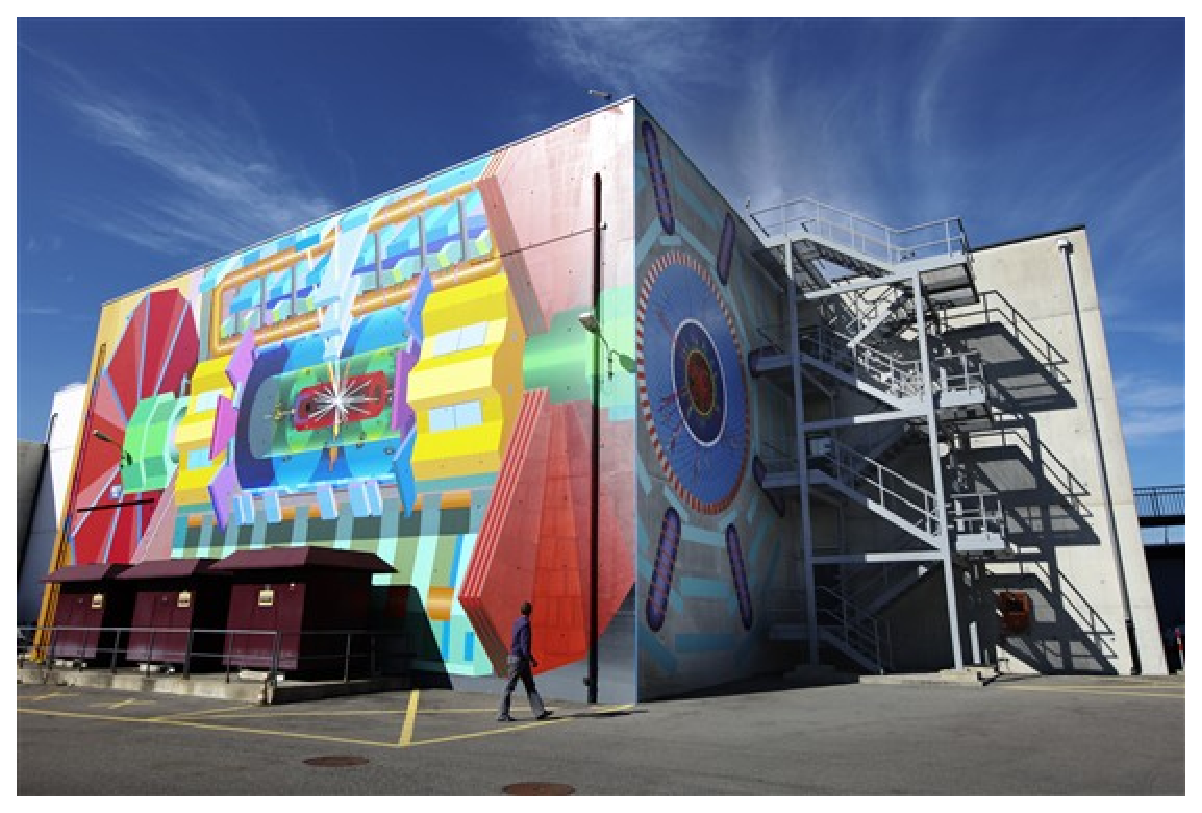
\includegraphics[width=0.47\textwidth]{detector/figures/mural}}
	\subfigure[]{\label{fig:lhcdraw}
  	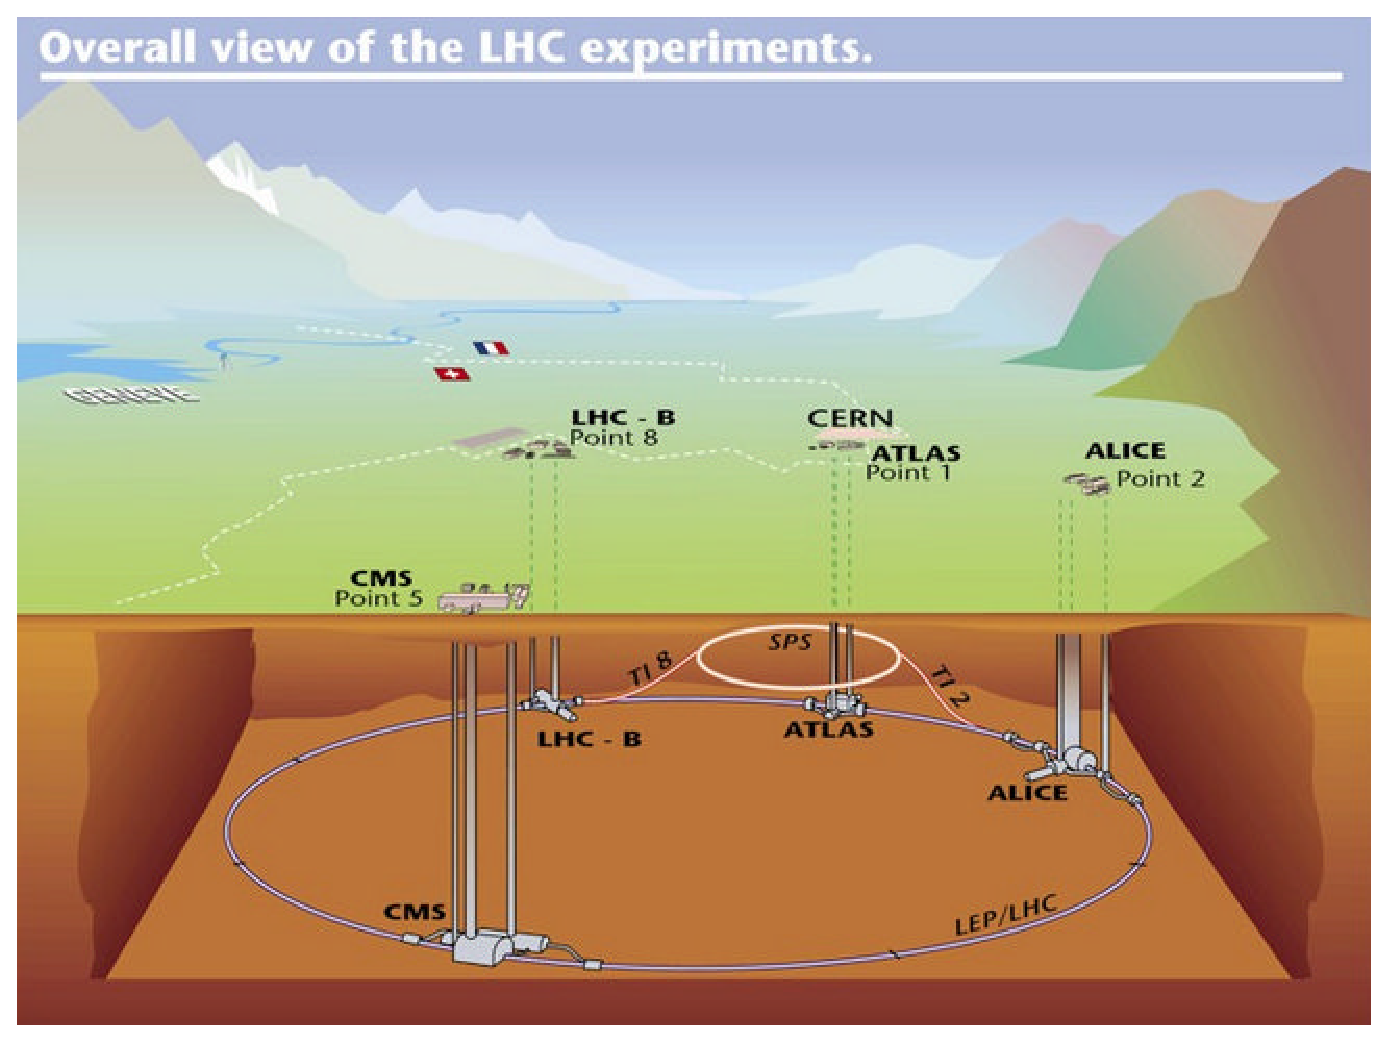
\includegraphics[width=0.42\textwidth]{detector/figures/lhc_diagram}}
	\caption[bla]{Left: View of Point 1, just above the ATLAS cavern, with a mural painting 
        of the detector, reproduced at a scale of about 1:3
        by artist Josef Kristofoletti\footnotemark.
        Right: A drawing of the LHC complex.\label{fig:nicepics}}
\end{center}\end{figure}

The collider accelerates protons up to 4~\tev, but is designed to reach 7~\tev\ per beam
when it will be operated at his full potential. This energy is achieved
through various steps, shown in Figure~\ref{fig:lhcring}.
To start with, protons are extracted from Hydrogen gas and injected in the first machine, the linear 
accelerator LINAC2 that starts the acceleration chain. When protons reach
an energy of 50~\mev\ they are injected into the Proton Synchrotron Booster
(PSB) and accelerated up to the energy of 1.4~\gev. The second circular
accelerator, the Proton Synchrotron (PS) brings the energy of the protons
to 25~\gev\ previous to injecting them into the last machine before the LHC,
the Super Proton Synchrotron (SPS). Protons of 450~\gev\ finally enter the
LHC where they are boosted to energies of up to 4~\tev.
The four main LHC experiments are shown on the collider ring.

\begin{figure}[tb]\begin{center}
	\subfigure{
  	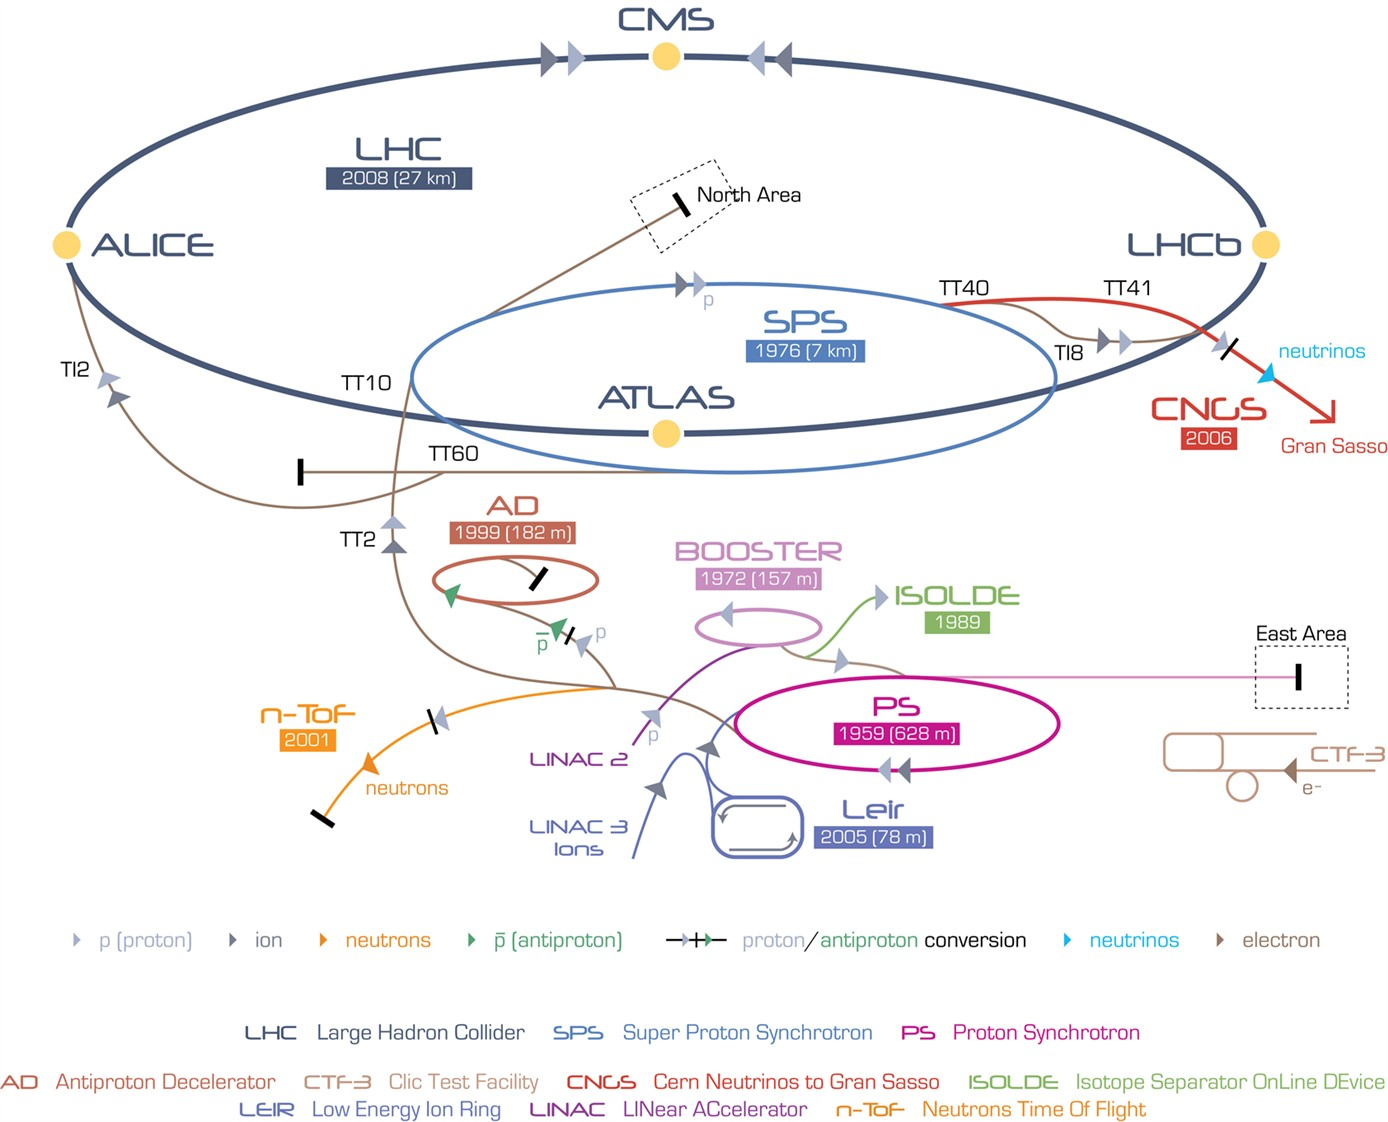
\includegraphics[width=0.8\textwidth]{detector/figures/ring.eps}}
	\caption{A schematic showing the accelerator complex at CERN.\label{fig:lhcring}}
\end{center}\end{figure}


\footnotetext{More info at: \url{http://www.atlas.ch/mural/}.}

The LHC is composed of eight arcs 2.7~km long, each of which contains 154 dipole 
magnets, whose function is to  bend the beams along the circular trajectory, and
49 quadrupole magnets, that focus the beam. These superconducting magnets operate
at a temperature of 1.9~K, maintained by means of liquid Helium vessels.
Eight insertions are placed inbetween the arches. Each insertion has a specific
role that characterizes its design and can be injection, beam dumping, beam cleaning,
or ``physics'', i.e. make the beams collide within an experiment.

First proton beams were circulated on 10th September 2008 and right on the verge of
getting the first collisions at a \cme $\rts=900\gev$ nine days later, an electrical
connection joining superconducting wires of a dipole and a quadrupole
failed. This caused the release of liquid Helium in the insulating vacuum,
resulting in an explosion that severely damaged the machine.
After more than one year devoted to repair the damage and consolidate the security,
on 30th November 2009 the LHC became the world's highest energy particle 
accelerator\footnote{\url{http://press.web.cern.ch/press/PressReleases/Releases2009/PR18.09E.html}}:
\begin{quotation}\small
Geneva, 30 November 2009. CERN's Large Hadron Collider has today become the world’s highest energy particle accelerator, having accelerated its twin beams of protons to an energy of 1.18 TeV in the early hours of the morning. This exceeds the previous world record of 0.98 TeV, which had been held by the US Fermi National Accelerator Laboratory’s Tevatron collider since 2001. It marks another important milestone on the road to first physics at the LHC in 2010.
\end{quotation}


One of the main characteristics for an accelerator is the luminosity, the 
instantaneous luminosity $\mathcal L$ being defined as 
\begin{equation}\label{eq:lumiN}
\mathcal{L}\times\sigma=\dfrac{dN}{dt}=f\times n\dfrac{N_1\times N_2}{A}\times\sigma.
\end{equation} 
Here $dN/dt $ is the event rate of a certain process and $\sigma$ is its cross 
section. This rate is directly proportional to the the frequency $f$, the number 
of bunches $n$ and the number of particles in the two bunches $N_1, N_2$, and
inversely proportional to the beam cross-section $A$.
The instantaneous luminosity is measured by dedicated subdetectors that are
described in Section~\ref{sec:forward}.

Integrating over the accelerator active time (a ``fill'', when stable beams are kept
colliding) gives the \textit{integrated luminosity}, relating the total number 
of produced events $N_{tot}$ to the cross-section:
\begin{equation}\label{eq:intLumi}
\int \mathcal L dt  = \dfrac{N_{tot}}{\sigma}.
\end{equation}




%http://accelconf.web.cern.ch/accelconf/IPAC2013/papers/moyab101.pdf
%http://cerncourier.com/cws/article/cern/54381

\begin{table}\centering
	\begin{tabular}{lllll}\toprule
        Parameter                       & designed      &       2010 &  2011     &   2012\\ \midrule
        Beam energy (\tev/c)            & 7             & 3.5        & 3.5       & 4    \\
        Beta function $\beta*$ (m)      & 0.55          & 2.0/3.5    & 1.5/1.0   & 0.6  \\
        Max. No. bunches/beam           & 2808          & 368        & 1380      &1380  \\
        Max. No. protons/bunch          & 1.15$\times10^{11}$ & 1.2$\times10^{11}$ & 1.45$\times10^{11}$ & 1.7$\times10^{11}$ \\
        Bunch spacing (ns)              & 25            & 150       & 75/50        & 50 \\
        Peak luminosity (\cmm2\sm1)     & 1$\times10^{34}$& 2.1$\times10^{32}$& 3.7$\times10^{33}$& 7.7$\times10^{33}$\\
        Emittance $\varepsilon_{n}$ ($\mu$rad)&3.75     &   2.0      & 2.4      & 2.5   \\
        Max. $<\mu>$                    & 19            & 4             & 17         & 37       \\
	\bottomrule\end{tabular}\caption{Overview of some parameters for the LHC performance comparing the design values with their time
        evolution during the first long run operation in 2010-2013~\cite{Lamont}.}\label{tab:lhcpar}
\end{table}

\begin{figure}[tb]\begin{center}
	\subfigure[]{\label{fig:intlumi}
  	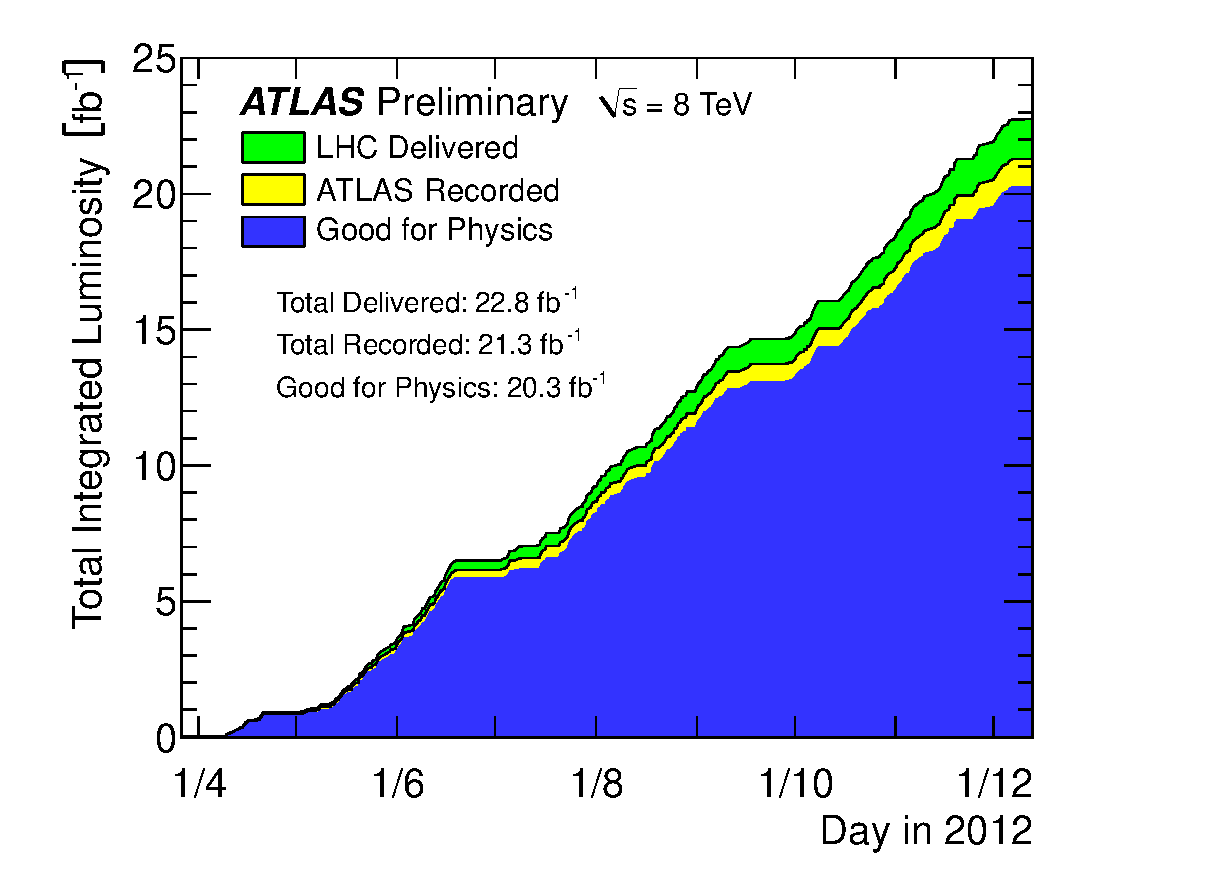
\includegraphics[width=0.48\textwidth]{detector/figures/intlumivstime2012DQ}}
	\subfigure[]{\label{fig:mu}
  	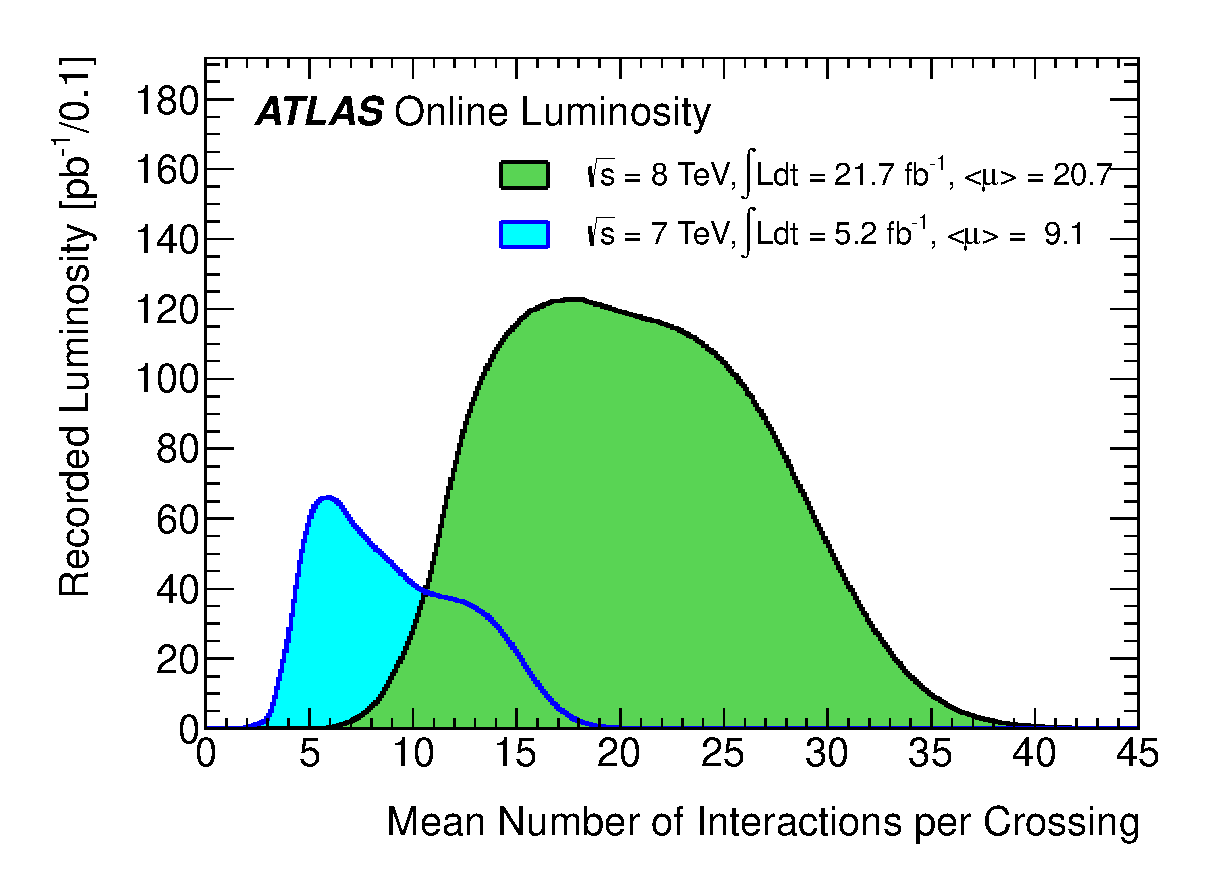
\includegraphics[width=0.48\textwidth]{detector/figures/mu_2011_2012-dec}}
	\caption{(a) Total integrated luminosity versus time delivered by the LHC to ATLAS (in green), recorded by the experiment 
        (in yellow) and selected as ``good data'' for analysis (in blue) for p-p collisions at \rts=8~\tev.
        (b) Mean number of interactions per beam crossing during 2011 and 2012 LHC runs, where 
        $\mu = \mathcal L\times \sigma_{\rm inelastic}/f$ depends on the instantaneous luminosity $\mathcal L$, the p-p inelastic
        cross section $\sigma_{\rm inelastic}$ and the revolution frequency $f$.~\cite{lumi}}
%Number of Interactions per CrossingMore details on this can be found in arXiv:1101.2185. 
\end{center}\end{figure}

In 2010 ATLAS collected about 45~\ipb of p-p collision data at \rts=7~\tev, and in
2011 reached about 5~\ifb of the same data.
In 2012, with  \rts=8~\tev\ collisions, LHC reached a peak luminosity of 7.7$\times10^{33}$~\cmm2\sm1\ which is
more than half the design luminosity, as shown in Table~\ref{tab:lhcpar} together
with other parameters relevant for the accelerator performance. 
Over 2012, the last
year of data taking before the long shutdown\footnote{LHC terminated the p-p program
at the end of 2012, operated proton-heavy ion collisions for two months at the beginning
of 2013 and then stopped for what is called the first long shutdown. During this two-years
time the accelerator and the experiments as well will undergo substantial maintenance and 
upgrade works, in order to be re-operated in 2015 with higher performance at a higher
\cme for particle collisions.},
ATLAS collected about 20~\ifb\ of p-p collision data at \rts=8~\tev.
Figure~\ref{fig:intlumi} shows the delivered luminosity from the start of stable beams until beam dump and the luminosity recorded by
ATLAS during stable beam conditions, the difference with respect to the delivered luminosity being due to Data AQuisition (DAQ)
inefficiencies. Of the recorded luminosity, only a part is usable for analysis, and is what is called ``good data'', i.e. 
the data that satisfy Data Quality (DQ) requirements assessed after reprocessing (see Section~\ref{sec:daq}).

In order to increase the luminosity LHC operates with a high number of protons per bunch as well as a high
 number of bunches per beam and reduces the inter-bunch latency time.
This overall defines a set of challenges that physics analysis will face associated to the high luminosity.
Even at the detector design stage, the high frequency of collision environment foreseen influenced
the choice of radiation resistance material for the experiment sub-systems. Concerning directly the physics
%instead we can list the main problematics as being \textit{underlying events} and \textit{pile-up}
instead, the main problematic is \textit{pile-up}.

Pile-up events are distinguished between \textit{in-time} and \textit{out-of-time} pile-up. The first ones come 
from the multiple inelastic scatterings of protons in the same bunch, as if we consider a cross-section of 80~mb
at the nominal luminosity of $10^{34}$~\cmm2\sm1 the number of events per second will be something like
a billion. This translate, at a collision frequency of one crossing every 25~ns, to about 20 interactions per
crossing that will be detected simultaneously. A useful observable to estimate in-time pile-up is
the number of reconstructed primary vertices (see Section~\ref{sec:primaryvertex}) $N_{\rm PV}$.
In addition, on the other hand, the inter-bunch time interval is so short
that the electronics reading the detector might not keep up with the frequency of collisions, leading to the
cumulation of events that happened in different beam crossings. This is the effect we refer to as 
out-of-time pile-up, and a good estimator for it is the average number of p-p interactions
per bunch crossing at the time of the event, $<\mu>$, which recalling Equation~\ref{eq:lumiN} is defined as:
\begin{equation}\label{eq:mu}
<\mu> = \dfrac{LA}{nf},
\end{equation}
with $L$ being the average instantaneous luminosity over a time period $\Delta t\gg 600$~ns.
The maximum values reached by the variable $<\mu>$ during the three years of data taking
are reported in Table~\ref{tab:lhcpar}.

Finally, ATLAS makes use of a three-level trigger system (described in Section~\ref{sec:trigger}) to identify
and record only the events of interest, while the pile-up issues are dealt with at the analysis 
reconstruction level.



\section{The ATLAS detector}\label{sec:atlas}

ATLAS (A Toroidal LHC ApparatuS)~\cite{Aad:2008zzm} is a general purpose experiment
aimed at exploring a vast range of physics scenarios and designed to measure the particles
produced in p-p collisions at the LHC at unprecedented energies and instantaneous luminosities. 
It is the biggest detector of its kind ever built (it's 46~m long and 25~m high) is characterized by
a full coverage of the space around the p-p interaction point and complete
containment of the particles produced in the collision. Different subsystems are
layered concentrically one after the other, each of them pursuing a specific task. 
Right around the interaction point
(IP) where the LHC makes protons collide there is the Vertex Detector, reconstructing
charged particles trajectories that are bent by the first solenoid magnet surrounding
the Vertex Detector. Particles going through it then encounter the two calorimeter systems,
the Electromagnetic and the Hadronic one. Muons are the only particles that will pass
the calorimeters material (beyond neutrinos) and a dedicated Muon Spectrometer is the last
piece of detector, embedded in a huge toroidal magnet. The detector complex is presented
as a schematic in Figure~\ref{fig:atlas}, and a drawing of particle detection in the various
subdetector systems is shown in Figure~\ref{fig:detection}. 

\begin{figure}[htb]\begin{center}
	\subfigure{
  	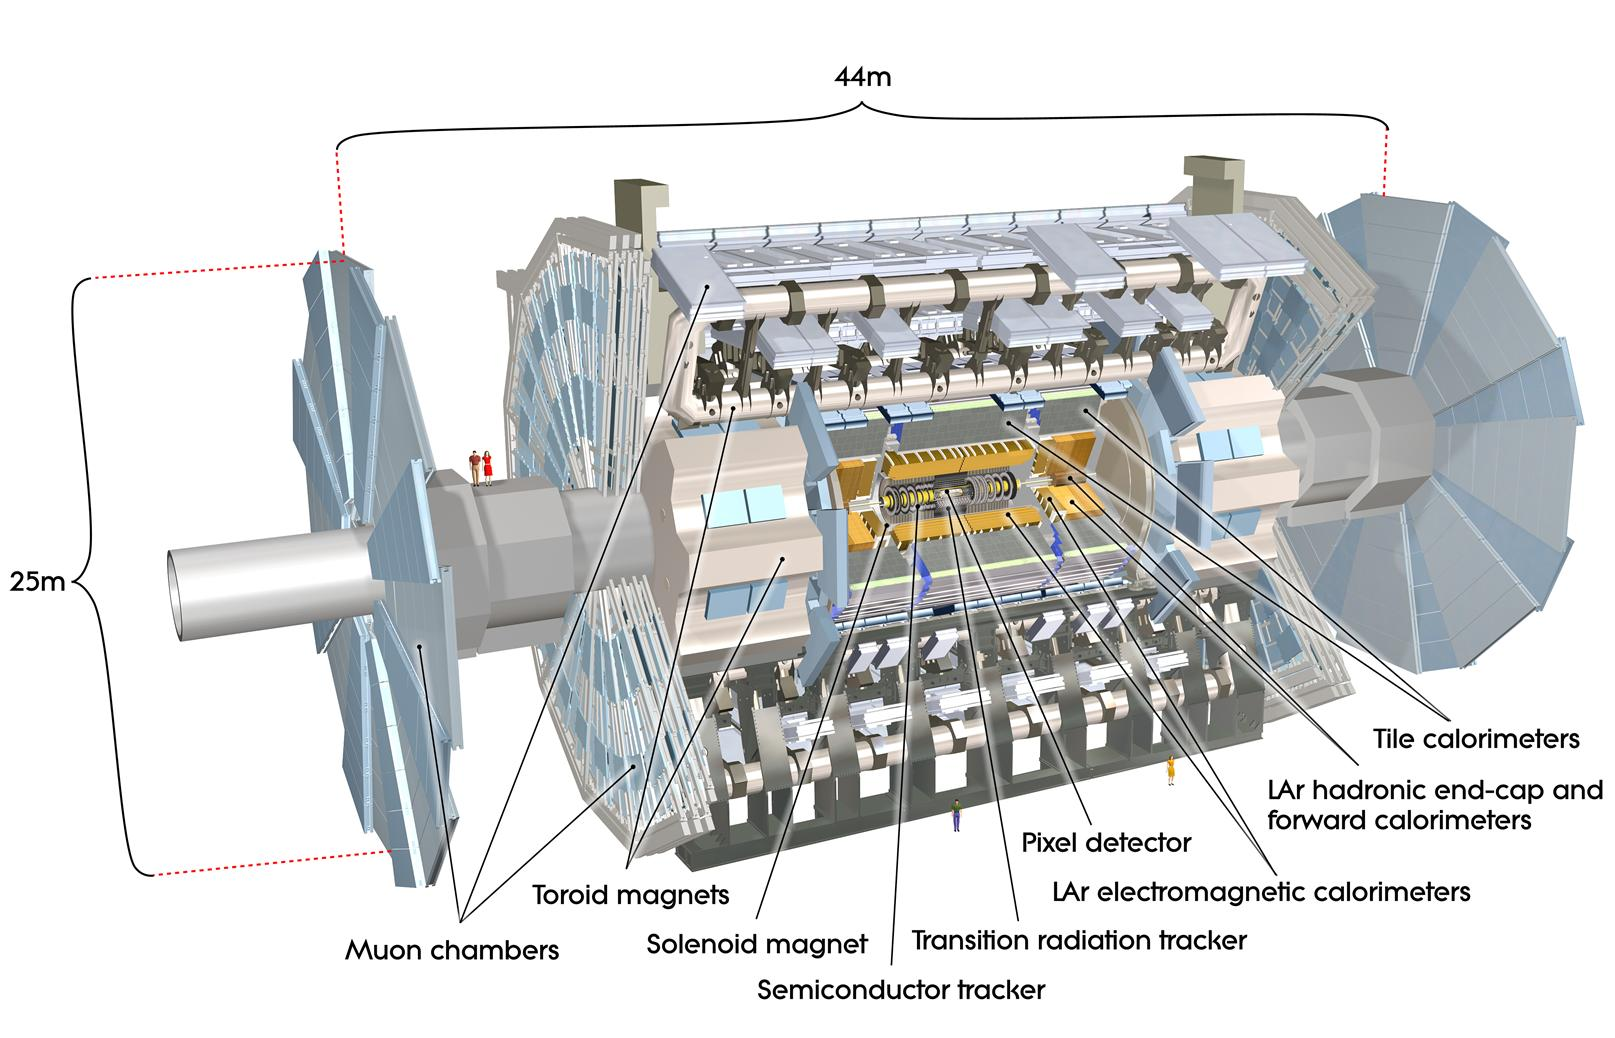
\includegraphics[width=0.9\textwidth]{detector/figures/atlas}}
	\caption{Schematic drawing of the ATLAS experiment. The detector subsystem are indicated as well as the total dimensions.\label{fig:atlas}}
\end{center}\end{figure}

\begin{figure}[htb]\begin{center}
	\subfigure{
  	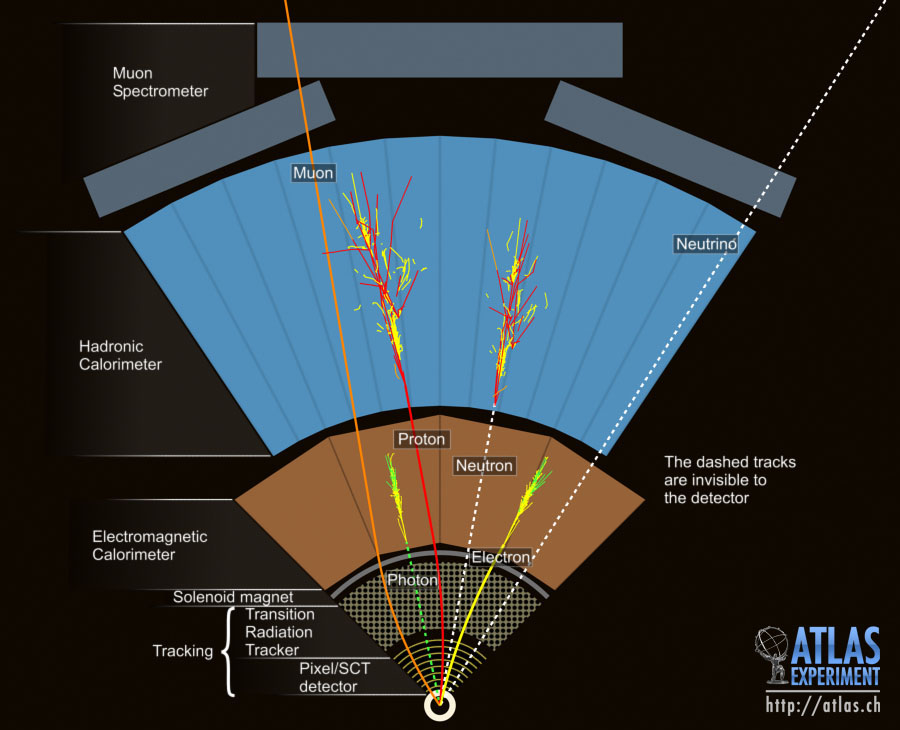
\includegraphics[width=0.75\textwidth]{detector/figures/detection}}
	\caption{Drawing of the detection of particles going from the interaction point through the whole detector.\label{fig:detection}}
\end{center}\end{figure}


\subsection{Coordinate system}

Protons from the two circulating beams are made to collide in the center of the ATLAS detector, in the region
that takes the name of Interaction Point (IP). The IP is taken as the origin of a three dimensional XYZ right-handed
coordinate system. The Z axis is tangent to the trajectory of the beams while the XY plane is perpendicular to
it and defines a symmetry plane for the detector, dividing it into the $A$ and $C$ sectors, respectively in the
positive and negative Z semi-axes. Figure~\ref{fig:coord} shows a schematic of the coordinate system.

\begin{figure}[tb]\begin{center}
	\subfigure[]{\label{fig:coord}
  	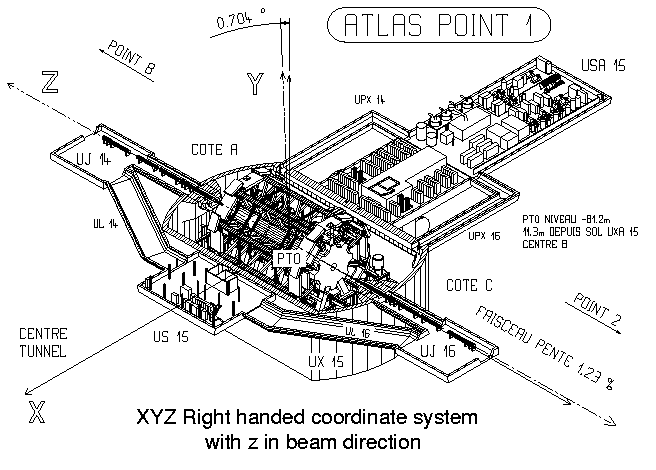
\includegraphics[width=0.6\textwidth]{detector/figures/coord}}\hskip3ex
        \subfigure[]{\label{fig:spherical}
  	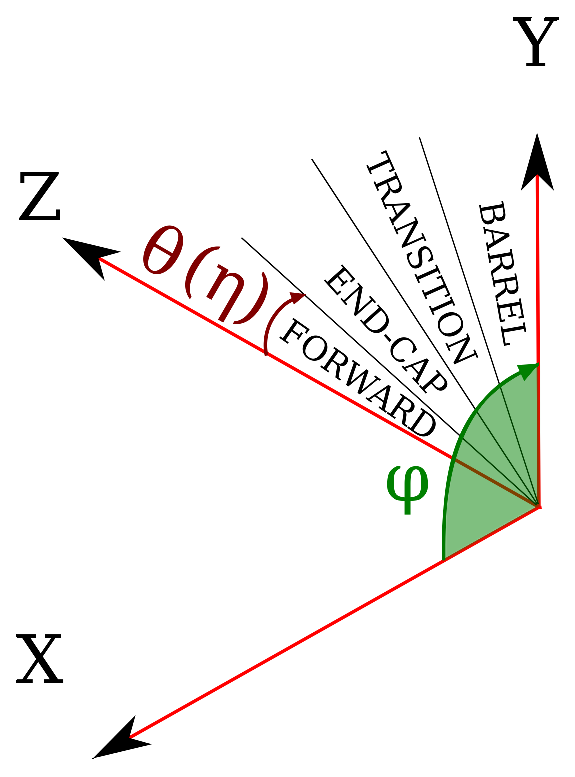
\includegraphics[width=0.3\textwidth]{detector/figures/spherical}}
	\caption{(a) Drawing of the ATLAS experiment with the cartesian coordinate system. The positive X axis points towards the center of the LHC
        ring. The positive Z axis points todards the anti-clockwise circulating direction of beam 2. (b) Simple schematic showing the spherical coordinates and the
        region definition in terms of the absolute value of the pseudorapidity $\eta$. These regions are symmetrical with respect to the transverse
        XY plane.}
\end{center}\end{figure}

In terms of polar coordinates, the Z axis is again along the beam axis and in the transverse plane 
the $R$ and $\phi$ coordinates are defined with $\phi$ ranging between 
$-\pi$ and $+\pi$ with respect to the X axis. In terms or spherical coordinates (see Figure~\ref{fig:spherical}),
the radial vector $R$ originates from the IP,  the azimuth $\phi$
is the same as the polar angle $\phi$, 
and the polar angle $\theta$ is measured with respect to the Z axis and
ranges between 0 and $\pi$. 

Since the interaction initial energy is unknown, being dependent on the parton distribution functions for the proton
energy, it is useful to define the transverse component of variables of 
interest\footnote{These quantities transverse initial value will be, indeed, zero, as the protons are accelerated along the Z axis.}  
like the energy and the momentum, being taken as the projection on the XY plane:

\begin{equation}\label{eq:transv}
\et = E\sin\theta, \qquad \pt = p\sin\theta.
	\end{equation}

Another common variable used at hadron colliders to describe the polar distribution and preferred to the simple
polar angle $\theta$ is the pseudorapidity $\eta$:
\begin{equation}\label{eq:pseudorapidity}
        \eta \equiv -\ln\bigg(\tan\frac{\theta}{2}\bigg);
	\end{equation}
which, for relativistic regimes, is equal to the rapidity $y$:
\begin{equation}\label{eq:rapidity}
y \equiv \frac{1}{2} \ln \bigg(\frac{E+p_{Z}}{E-p_{Z}}\bigg);
	\end{equation}
and $\Delta y$ and $\Delta \eta$ are Lorentz invariant. The pseudorapidity is preferred
to the rapidity as it does not require knowing the particle mass but only its polar position.
The distance between two particles is often referred to in terms of $\Delta R$:
\begin{equation}\label{eq:deltar}
\Delta R = \sqrt{(\Delta\eta)^{2} + (\Delta\phi)^{2}}.
	\end{equation}


%since particles produced in collisions are not uniformely distributed in $\theta$. 
Figure~\ref{fig:spherical} shows how different pseudorapidity regions are named. Particles
along the Z axis have a pseudorapidity $|\eta|=\infty$, particles along the Y axis have
a pseudorapidity $|\eta|=0$. ATLAS has an excellent hermeticity and is able to cover 
pseudorapity regions up to $|\eta|=4.9$. Typically, physics analysis consider objects in
the pseudorapity region  $|\eta|<2.5$. For a quick visualization of the correspondence
in terms of polar angle distribution, some pseudorapidity values are reported in Table~\ref{tab:etatheta}.
%AAAAAAAAAAAAAAAAA add barrel forward blabla exact def


\begin{table}[htb]\centering\begin{tabular}{cccccccccc}\toprule
$\theta$ & 0$^{\circ}$ & 5$^{\circ}$ & 10$^{\circ}$ & 20$^{\circ}$ & 30$^{\circ}$ & 45$^{\circ}$ & 60$^{\circ}$ & 80$^{\circ}$ & 90$^{\circ}$ \\
$\eta$ & $\infty$ & 3.13 & 2.44 & 1.74 & 1.31 & 0.88 & 0.55 & 0.175 & 0\\\bottomrule \end{tabular}
\caption{Pseudorapidity vs polar angle values.}\label{tab:etatheta}\end{table}

\subsection{Magnets}\label{sec:magnets}

ATLAS is provided with four superconducting magnets that allow the measurement of
charged particles momenta by curving their trajectory. 

A central solenoid, 5.3~m long and 2.4~m in diameter, sits 
around the inner detector and produces a 2~T magnetic field along the direction
parallel to the beam axis. It is only 45~mm thick (equivalent to 0.66 radiation lenghts $X_0$)
and is cooled with liquid Helium, sharing the cryostat with the electromagnetic calorimeter.

Paired to the muon spectrometer, the superconducting air-core toroid magnet (Figure~\ref{magnets}) 
has an open structure with eight superconducting toroidal coils in the barrel part (each 25.3~m long, located
at the outer diameter of 20.1~m) and
two end-cap systems made of eight coils. The field strength varies strongly with $\phi$:
in the barrel region ($|\eta|<1.4$) is 1.5-5.5 Tesla$\cdot$m; in the end-caps ($1.6<|\eta|<2.7$) 1-7.5 is Tesla$\cdot$m. 
Such configuration of the magnets gives a field orthogonal to the muons trajectory.

\begin{figure}[hbt]\begin{center}
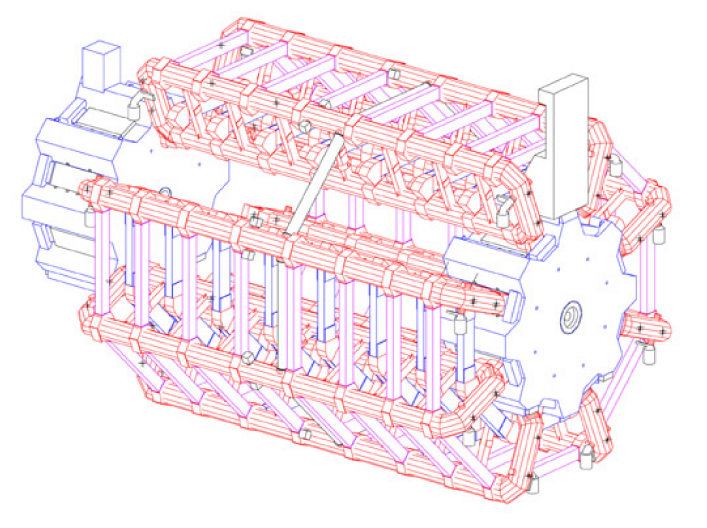
\includegraphics[width=.8\textwidth]{detector/figures/magnets}\caption{Toroidal magnet system.}\label{magnets}
\end{center}\end{figure}



\subsection{Inner detector}\label{sec:innerdet}

The Inner Detector (ID) is the subsystem closest to the IP and tracking charged particles arising from collisions allows for 
the measurement of their momentum and vertex reconstruction with excellent resolution. At the design choices level, radiation resistance had to
be taken into account, as well as reducing the amount of material to be placed in front of the calorimeters to avoid spoiling the energy measurement.
This quantity varies between 0.5 and 2.5~$X_0$ depending on the pseudorapidity region, most of it coming from supporting equipment. This material
is responsible for photon conversions and electron bremsstrahlung.

The ID is surrounded by the central solenoid magnet (Section~\ref{sec:magnets}) and is composed by three subsystems, 
from the closest to the furthest from the IP: the pixel detector, the SemiConductor Tracker (SCT) and
the Transition Radiation Tracker (TRT).
%silicon strip detector and a straw detector (Figures~\ref{fig:innerdet1} and~\ref{fig:innerdet2}).

\begin{figure}[tb]\begin{center}
	\subfigure[]{\label{fig:innerdet1}
  	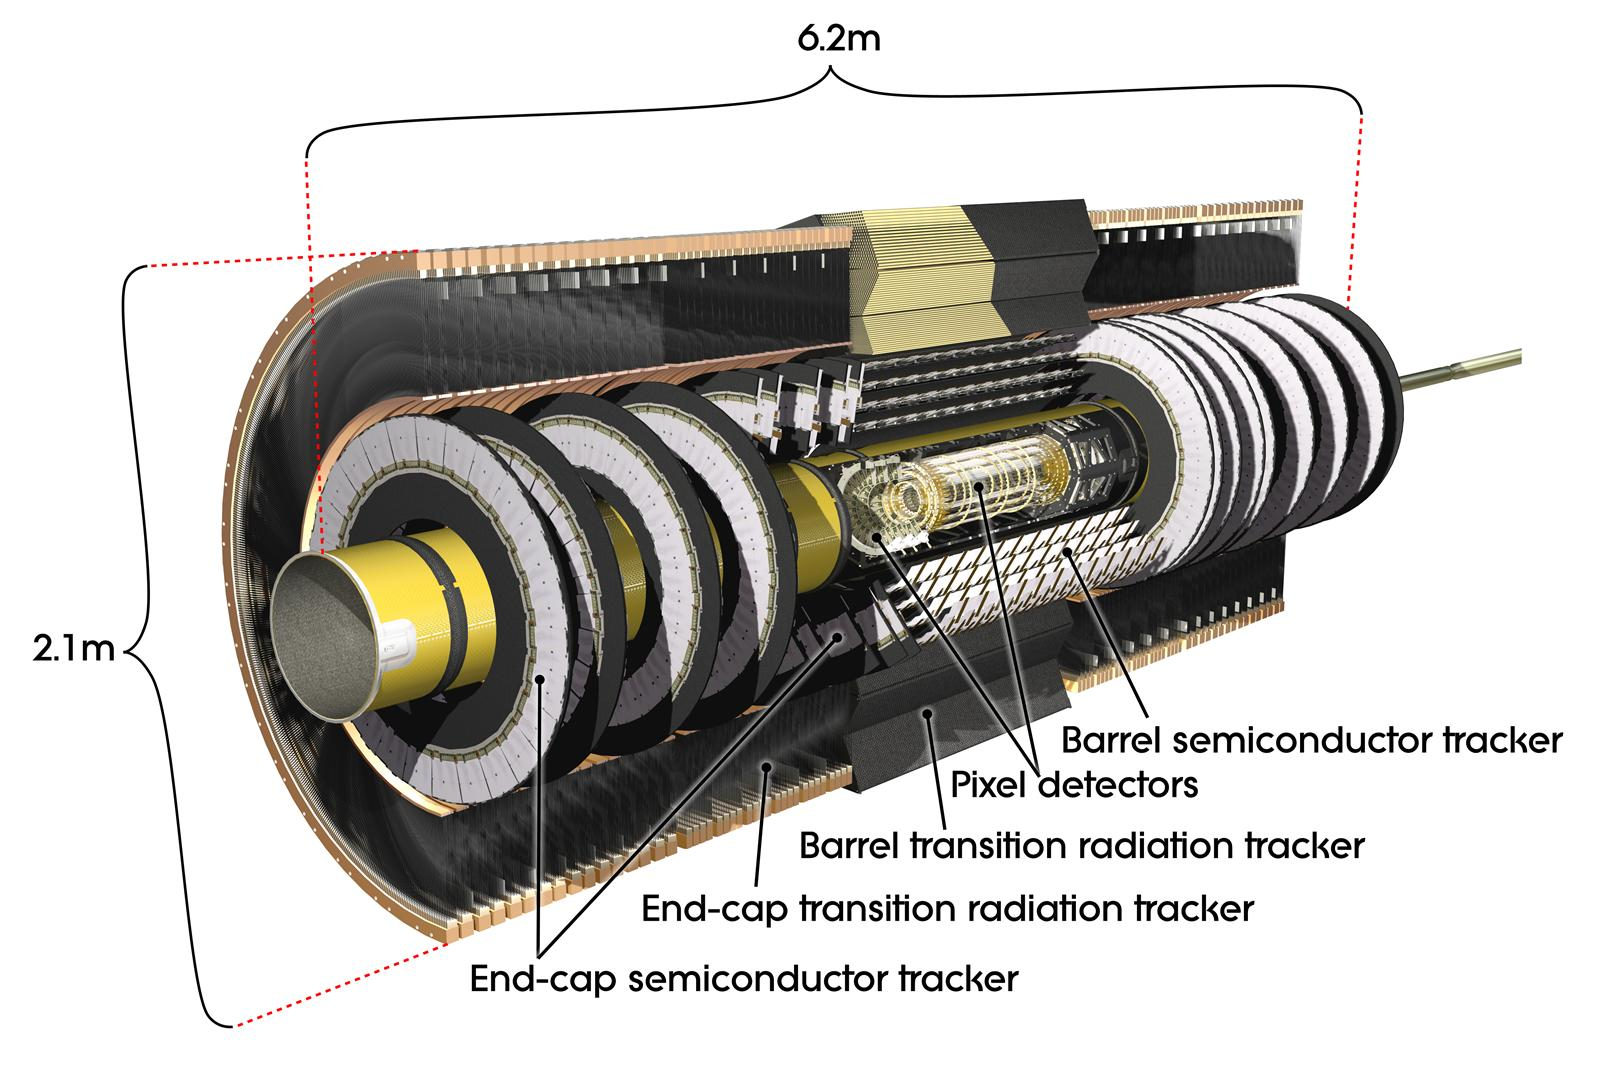
\includegraphics[width=0.6\textwidth]{detector/figures/innerdet}}
	\subfigure[]{\label{fig:innerdet2}
  	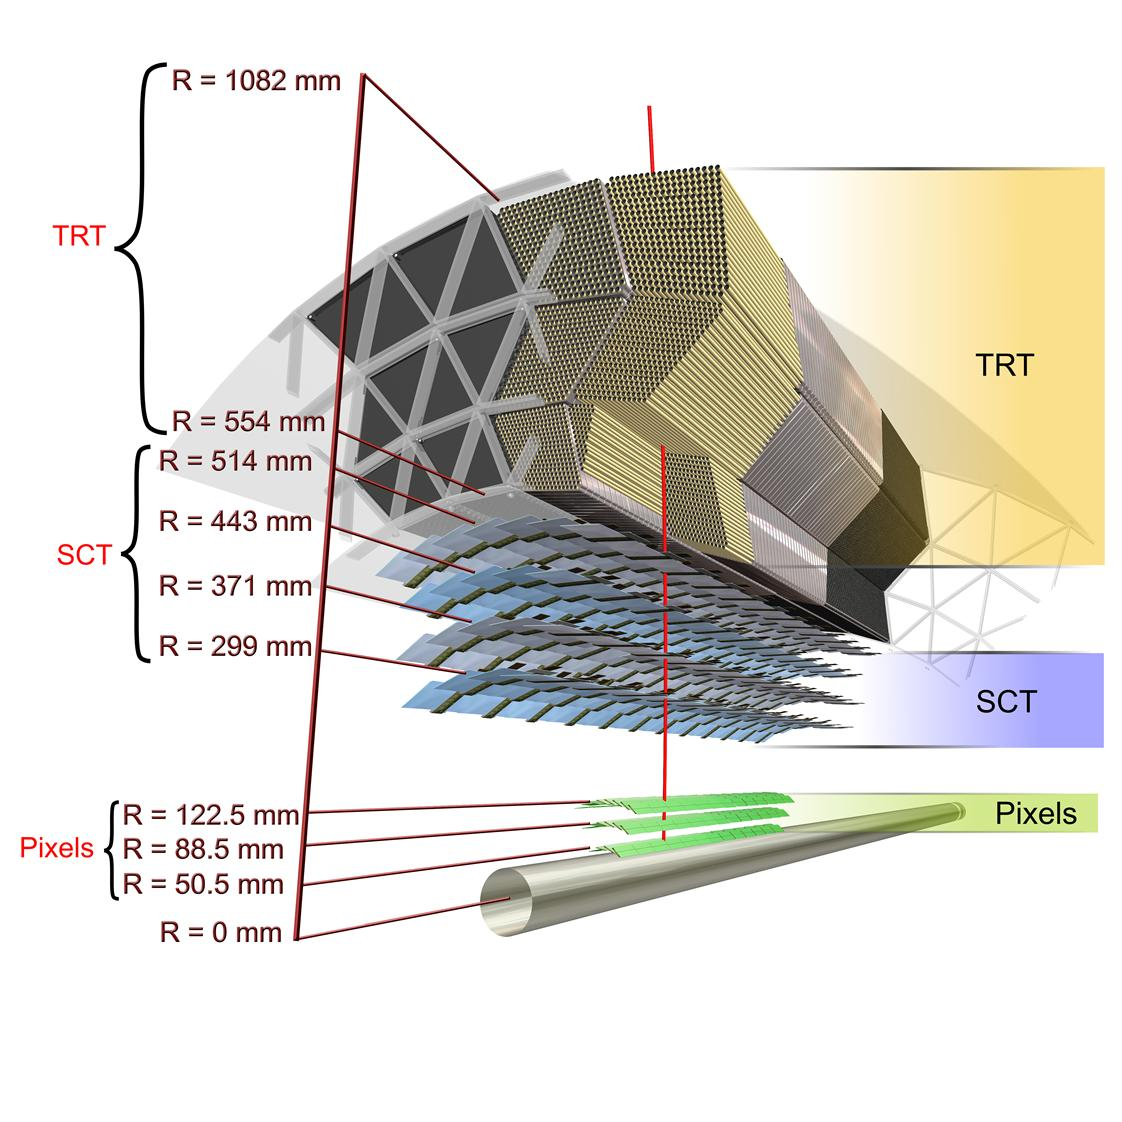
\includegraphics[width=0.37\textwidth]{detector/figures/innerSection}}
	\caption{(a) Schematic of the ID system. (b) Detailed schematic of the barrel section of the ID showing the
        three subsystems and reporting the distance to the center of the beam pipe.}
\end{center}\end{figure}


\subsubsection{Pixel detector}

The first subsystem covers the region $|\eta|<2.5$ and  is composed by three cylindrical layers in the barrel region, each of them distant from the beam by
50.5~mm, 88.5~mm and 122.5~mm respectively, and by three concentric discs in the end-cap region, each of them distant from the beam by
49.5~mm, 58.0~mm and 65.0~mm respectively.
Each silicon pixel has a size of 50$\times$400~$\mu$m$^{2}$ and is 250~$\mu$m thick, 
with in total $\sim$80.4 million readout channels to achieve a very fine granularity.
The precision is of 10~$\mu$m in $R\phi$ and 115~$\mu$m in Z and $R$ in the barrel and end-cap
region respectively.

The very first layer is called $B-$layer as, thanks to its position really close to the IP,
allows for the reconstruction of secondary vertices associated with the production of
 short lived particles such as $B-$hadrons. This information is very useful to identify
jets originating from the fragmentation of $b$ quarks.

\subsubsection{Semiconductor tracker}

After the three layers of pixel detectors, come four layers of  silicon strip detectors. The SemiConductor
Tracker (SCT) also covers the region $|\eta|<2.5$ with a barrel and end-cap design similar to the 
pixel detector one, being composed by eight silicon strips (two per layer) 128~mm long and 80~$\mu$m large.
It makes use of $\sim$6.3 millions readout channels and the resolution achieved is of 17~$\mu$m 
in $R\phi$  and 580~$\mu$m in Z ($R$) in the barrel (end-cap) region.

By allowing for four redundant position measurements\footnote{One of the coupled layers is rotated of $40$mrad with respect
to the other, which is parallel to the axis, giving a small stereo angle for a redundancy in the $\phi$ coordinate measurement.}, 
the SCT contributes mainly to the momentum reconstruction.

%Silicon has a band gap of just 3.6 eV, that is the minimum energy to create an electron/hole pair. Thus a minimum ionising particle creates around 80 electron/hole pairs per $\mu$m through primary and secondary ionisation.

\subsubsection{Transition Radiation Tracker}

In order to reduce the amount of material in front of the calorimeters, and to reduce the construction costs as well,
in the third subsystem the semiconductor technology has been substituted with straw detectors.
The Transition Radiation Tracker (TRT) consists of thin proportional chambers made of straw polyimide drift tubes, 4~mm in diameter.
The drift tubes are filled with a gas mixture composed of: 70\% Xenon, 27\% Carbon Dyoxide, 3\% Oxygen. The anode 
collecting the electrons from the ionized gas at the passage of the charged particle is made of
tungsten covered in gold.

In the barrel region the tubes are 144~cm long and placed parallel to the beam axis, while in the 
end-cap region they are 37~cm long and positioned radially in wheels, with layers of radiator foils alternated 
to layers of straws. The resolution achieved is of 130~$\mu$m in $R\phi$ and Z$\phi$  in the two regions respectively.
The covered pseudorapidity region is of $|\eta|<2.0$ and the readout is composed by $\sim$351000 channels.

About 36 measurements per track are taken, and since each channel provides two independent thresholds per hit,
it is possible to discriminate between electrons and pions, since the former will more likely reach the
high threshold.

In the end, the combination of the three ID subsystems gives very precise $R\phi$ and Z measurements, as well as good track pattern recognition.
The resolution on the transverse momentum, measured with cosmic muon calibration runs~\cite{id_cosmic}, is:

\begin{equation}\label{eq:momentumres}
\frac{\sigma_{\pt}}{\pt}=P_1 \oplus P_2 \times \pt,
	\end{equation}
where $P_1=1.6\pm0.1\%$ and $P_2=(53\pm2)\times10^{-5}$~\GeV$^{-1}$. This means a 
resolution of~$\sim$1.6\% for tracks with $\pt\sim$1~\GeV\ and 
$\sim$50\% for tracks with $\pt\sim$1~\tev.


\subsection{Calorimeters}\label{sec:calo}

Particles leaving the ID and surviving the crossing of the central solenoid magnet
will face the calorimeter system, depicted in Figure~\ref{fig:calorimeters}.
The full system is characterized by a coverage
in pseudorapidity up to $|\eta|<5$ and an almost full coverage in $\phi$. With its 
22~$X_0$ and 24~$X_0$ radiation lengths of material in the barrel and end-cap regions respectively 
it is also able to stop most of the non-muon particles from the interaction.
Besides particles energy measurement, the calorimeters provide particle identification
information, discriminating electrons, photons and jets, and the determination
of the missing transverse energy.

Different technologies are used in the barrel, end-cap and forward regions for both the
electromagnetic and the hadronic calorimeters. All of them are sampling calorimeters,
with a dense medium acting as absorber to stop particles and start showers, and an
active material to detect the signal from ionization. For the electromagnetic calorimeters
and the forward hadronic calorimeter liquid argon is used as active medium, while the
barrel and extended-barrel hadronic calorimeter uses scintillating tiles.
The liquid argon is cooled at a temperature of about 88~K, with the use of two sets of cryostats:
the barrel electromagnetic calorimeter shares the cryostat with the central solenoid;
the end-cap and forward electromagnetic calorimeter and the hadronic end-cap calorimeter
share a cryostat in the foward region.

\begin{figure}[tb]\begin{center}
	\subfigure{
  	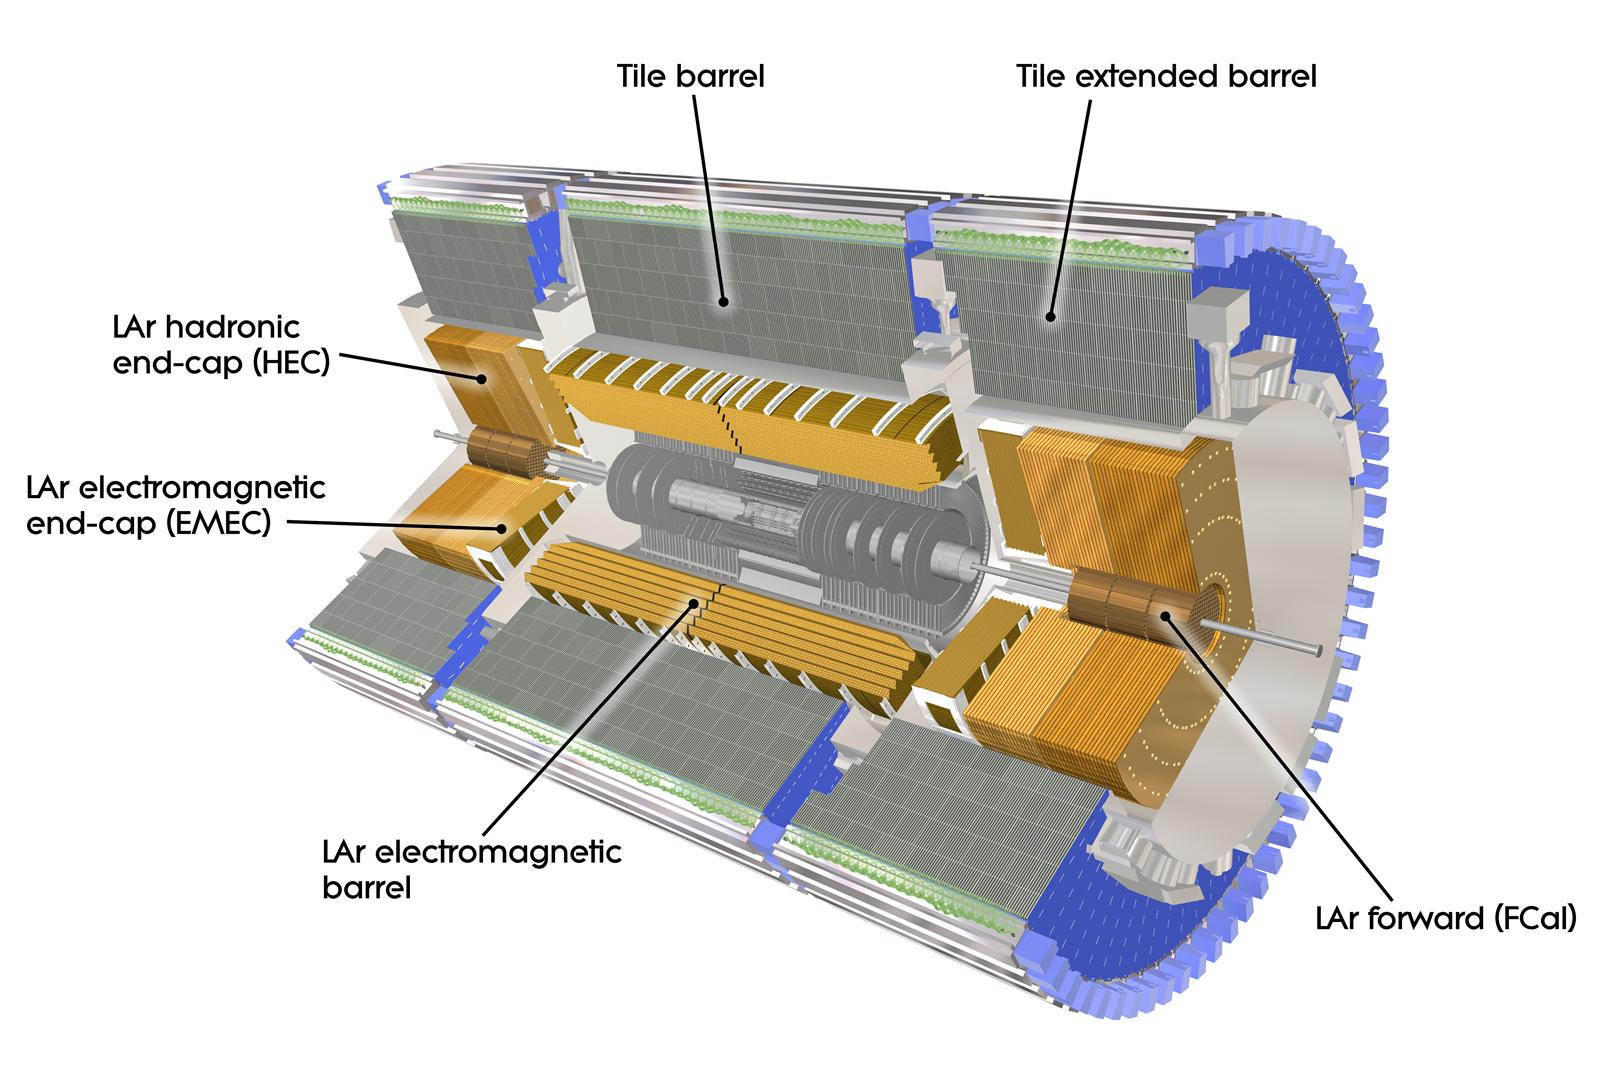
\includegraphics[width=0.8\textwidth]{detector/figures/caloBarrel}}
	\caption{Schematic of the calorimeter complex of the ATLAS detector.\label{fig:calorimeters}}
\end{center}\end{figure}

Particles interact both with the passive and active material, but only the energy released
in the active samples will be detected. 
%The balance, chosen at the design stage, between
%the two elements will determine how much the calorimenter compensate for the 
The processes involved in the shower formation are several and mainly electromagnetic.
Photons in matter can undergo the photoelectric effect, Compton scattering and $\gamma \to \epem$
pair formation. The general contribution of these processes depends both on the photon energy
and on the atomic number $Z$ of the material, and is shown in Figure~\ref{fig:photonsmatter}.
Electrons and positrons can ionize atoms and molecules, produce bremsstrahlung $\epm \to \epm + \gamma$
and emit Cerenkov radiation. Unless the calorimeter has been specifically designed for it,
 Cerenkov radiation does not contribute much, while ionization is the main process for energies
up to $\sim 100$~\mev, where bremsstrahlung starts to dominate.

In general, these cascade of events
continues until a certain threshold is reached, and the final number of particles
produced is proportional to the energy of the first particle originating the shower.

\begin{figure}[tb]\begin{center}
	\subfigure{
  	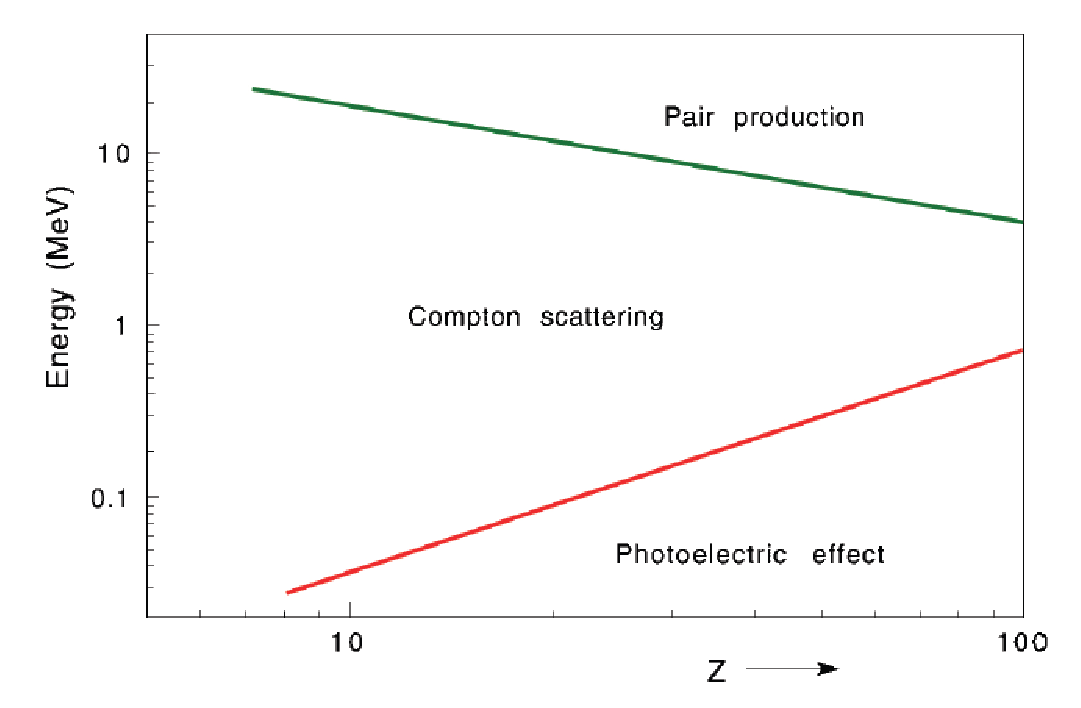
\includegraphics[width=0.6\textwidth]{detector/figures/photonsmatter}}
	\caption{Domains in term of photon energy and $Z$ number of the absorber material
        in which photoelectric effect, Compton scattering and pair production are the 
        favorite processes for energy loss~\cite{Wigmans}.\label{fig:photonsmatter}}
\end{center}\end{figure}

Also hadrons interact with matter, either ionizing it (if charged) or by nuclear interactions.
The problem of the latter process is that this energy release is often not directly detectable,
like in nuclear breakups and excitations, and is therefore called ``invisible energy''.
Secondary hadrons will be produced, forming the hadronic part of the shower, but sooner
or later something like $\pi^0\to \gamma\gamma$ will happen and the shower will
develop electromagnetically further on.

The average fraction of electromagnetic and hadronic shower components is a characteristic
of the sampling calorimeter and depends on the choice of the passive and active material
and on the design. Calorimeters are said to be {\it non-compensating} if, like the ATLAS
calorimeters, the detection of hadronic showers is less efficient than the one of 
electromagnetic showers. Calorimeters with a similar response for the two components
are called  {\it compensating}, while calorimeters more efficient when revealing
hadronic showers are  {\it over-compensating}.

%The distinction between electromagnetic and hadronic calorimeters is due to the different phenomenology of the physics involved. The development of electromagnetic showers from an incident electron or photon is well understood and for particles with equal incident energy the variations in shape and measured energy of the showers are quite small. The size of the shower is linearly dependent on the radiation length $X_{0}$ of the material entered, while the size of hadronic showers depends linearly on the nuclear interaction length\footnote{The nuclear interaction length is the average distance traveled by hadrons before inducing a nuclear reaction.} $\lambda_{int}$ of the material. 

The performance for the energy resolution is parametrized by the following formula:
\begin{equation}\label{eq:resolution}
\frac{\sigma_{E}}{E} = \frac{S}{\sqrt{E}}\oplus\frac{N}{E}\oplus C,
\end{equation} 
where the terms of the sum correspond, respectively, to a ``stocastic'' term related to how shower develops in the sampling calorimeter; to a ``noise''
term including the contribution from electronic noise and pile-up energy fluctuation; 
to a systematic term that depends on calibration, shower containment, inactive material and on the
linearity of the response as well. 

The goal energy resolution for the liquid argon calorimeters is~\cite{lar_readiness}:
\begin{equation}
\frac{\sigma_{E}}{E}=\frac{10\%}{\sqrt{E}} \oplus\frac{170\MeV}{E} \oplus 0.7\%,
\end{equation}
while for the hadronic barrel calorimeter is~\cite{tile_readiness}:
\begin{equation}
\frac{\sigma_{E}}{E}=\frac{50\%}{\sqrt{E}} \oplus 5\%.
\end{equation}
Test-beam runs to measure the response of the two calorimeters to electrons
and single pions respectively have shown results comparable to the goal resolutions.


\subsubsection{Electromagnetic calorimeter}\label{sec:emcalbarrel}

The electromagnetic calorimeter, also called LAr calorimeter (from Liquid Argon, the active material),
can measure electrons and photons energies in the range from 50~\mev\ to 3~\tev.
In the barrel region it is referred to as EMB (ElectroMagnetic Barrel), is 
divided into two identical semi-barrels EMBA and EMBC separated at Z=0 by a 6~mm
gap and covers the pseudorapidity region $|\eta|<1.475$. 
Two end-cap detectors (EMEC, ElectroMagnetic End-Cap), divided 
into two coaxial wheels, cover the pseudorapidity 
regions $1.375<|\eta|<3.2$. A pre-sampler, extended over 
$|\eta|<1.8$, stands in front of the EMB and allows for the measurement of
the energy the particles lost before reaching the EMB i.e. crossing the
material of the ID, the central solenoid and the cryostat.

Three longitudinal samples in the EMB are designed for different tasks. The first
sample, 4.3$X_0$ long, is finely segmented in $\eta$ to precisely measure
the direction in pseudorapidity of the particles with  thin readout strips
of $\Delta\eta\times\Delta\phi$ = 0.0031$\times$0.098. This helps for
photon/$\pi^{0}$ discrimination and as well for separate close-by $\gamma$s
from $\pi^{0}$ decay.
The second sample, 16$X_0$ long, contains the bulk of electrons and photons energy deposit. 
It is divided in towers with dimension $\Delta\eta\times\Delta\phi$ = 0.025$\times$0.0245
and provides the position measurement of the cluster. 
The  95\% of the energy of the shower is deposited in a matrix of 3$\times$7 
towers $\Delta\eta\times\Delta\phi$.
The third sample, 2$X_0$ long, is coarsely segmentes and collects the last bit of the longitudinal
development of the electromagnetic showers. Towers in this region have a dimension
of $\Delta\eta\times\Delta\phi$ = 0.05$\times$0.0245.

Also the EMEC is divided in three longitudinal samples (two in the region $1.375<|\eta|<1.5$),
and besides the lead, also the thickness of the liquid argon layers are varied in the
radial direction.

\begin{figure}[tb]\begin{center}
	\subfigure[]{\label{fig:calolar}
  	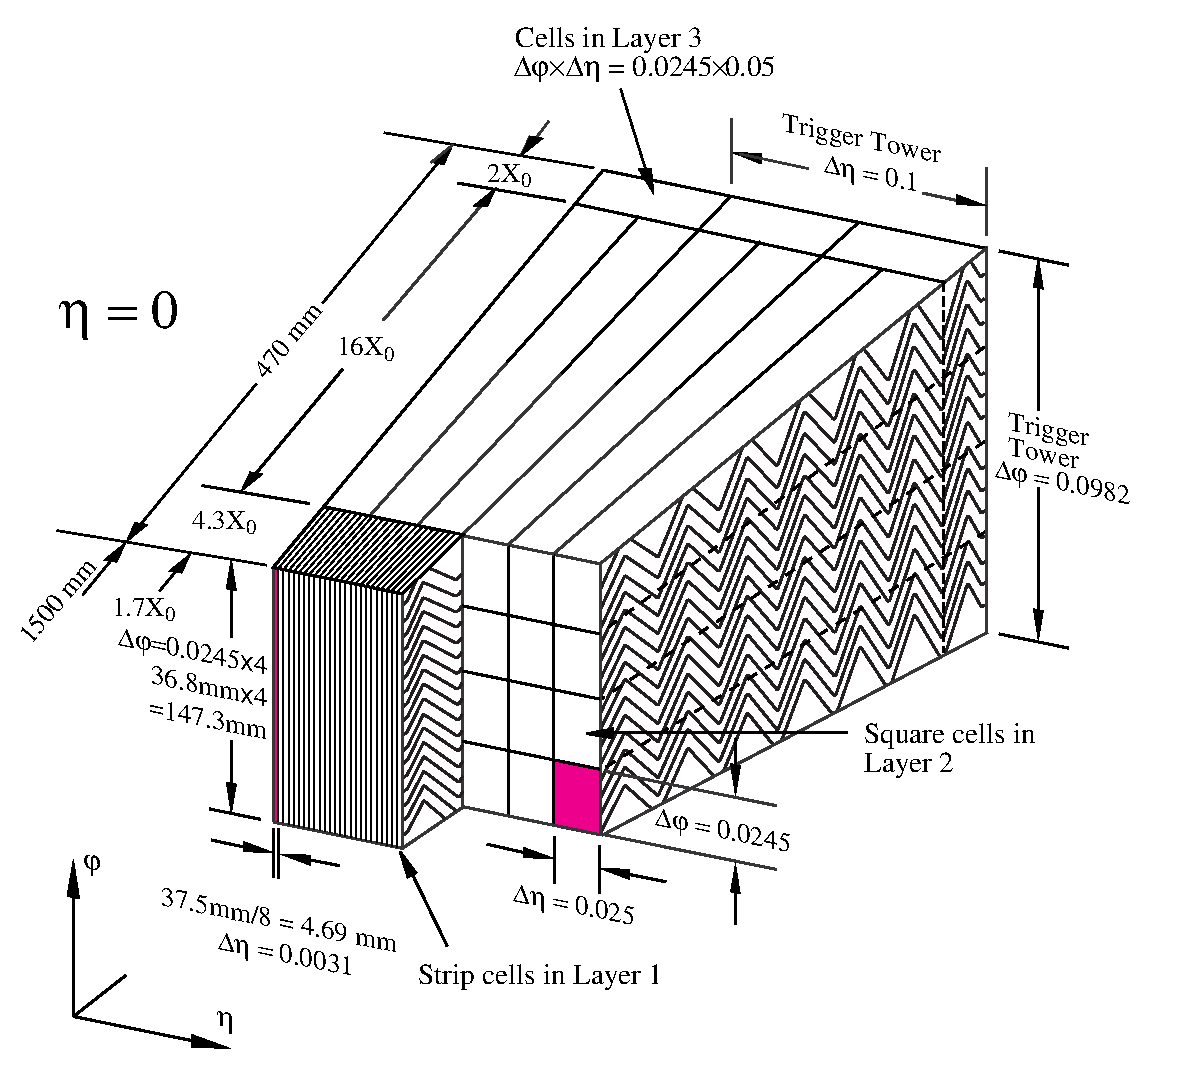
\includegraphics[width=0.48\textwidth]{detector/figures/caloLAr2}}
	\subfigure[]{\label{fig:calotile}
  	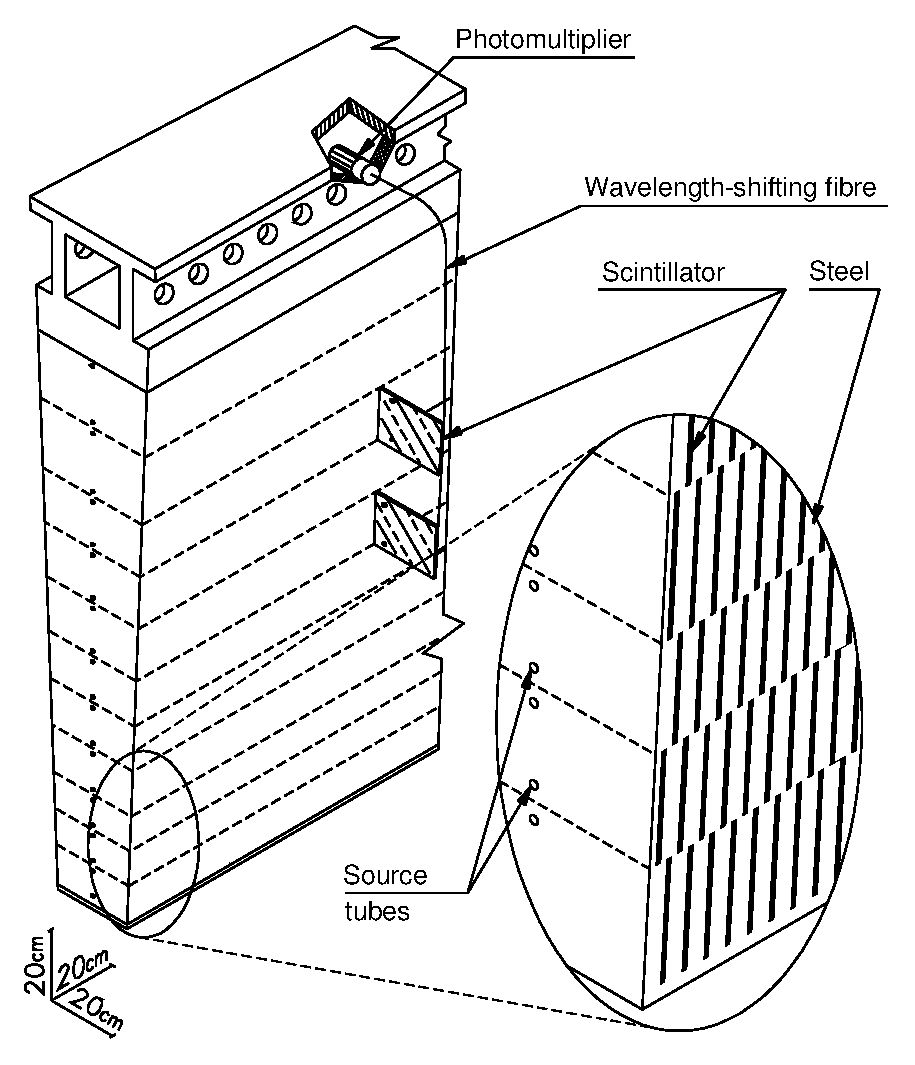
\includegraphics[width=0.38\textwidth]{detector/figures/caloTile}}
	\caption{(a) Schematic drawing of a module of the Electromagnetic barrel calorimeter. 
        (b) Schematic drawing of a module of the Hadronic barrel calorimeter.}
\end{center}\end{figure}


The absorbing material is lead shaped into an accordion geometry to achieve
full symmetry in $\phi$, as shown in the drawing of Figure~\ref{fig:calolar}.
Signal from the ionization produced in the liquid argon is collected
by an electrode in the middle of the active material region, fixed into
a honeycomb structure.

The thickness of the absorber layers depend on the pseudorapidity in
order to make particles entering the system with different incident 
angles cross the same amount of material.

\subsubsection{Hadronic calorimeters}\label{sec:hadcal}

Hadronic showers have typically a much longer shape than
electromagnetic ones, and need therefore in general more
interaction lenghts of material to be fully contained.
Hadronic calorimeters are therefore designed to completely
absorb high-energy hadrons, which will deposit only some (small) part of their energy 
in the electromagnetic calorimeter.



\subsubsection{Hadronic barrel calorimeter}\label{sec:hadcalbarrel}

The hadronic calorimeter in the barrel and extended barrel region, going up to
$|\eta|<1.7$, is made of scintillating tiles as active material with lead as absorber
and is commonly referred to with the name of TileCal. 
The light in the ultraviolet range that is generated in the tiles is collected through
wavelenght shifting optical fibre (Figure~\ref{fig:calotile}).

TileCal sits just after the electromagnetic
calorimeter and measures the energy and position of jets and isolated hadrons.
It is divided in depth in three layers with varying lenght (1.4, 4.1, 1.8 hadronic interaction
leghts $\lambda$ in the barrel and 1.5, 2.6, 3.3$\lambda$ in the extended barrel) and segmentation
($\Delta\eta\times\Delta\phi$ = 0.1$\times$0.1 in the first two layers,
$\Delta\eta\times\Delta\phi$ = 0.2$\times$0.1 in the third),
and in 64 slices in $\phi$, each of $\Delta\phi\sim0.1$.

The redout channels are grouped into cells that form a pseudo-projective geometry in $\eta$.

\subsubsection{Hadronic end-cap calorimeter}\label{sec:hadcalendcap}

The Hadronic End-Cap calorimeters (HEC) use copper as passive material and liquid
argon as active material, chosen for its radiation hardness in a region ($1.5<|\eta|<3.2$)
exposed to a significant amount of particle flux. Each HEC is composed by
two independent wheels with granularity varying with $\eta$: 
in $1.5<|\eta|<2.5$ $\Delta\eta\times\Delta\phi$ is 0.1$\times$0.1 in the first
two longitudinal layers,  0.2$\times$0.1 in the last one; in
$2.5<|\eta|<3.2$ $1.5<|\eta|<2.5$ $\Delta\eta\times\Delta\phi$ = 0.2$\times$0.2
in all the three samples.

The HECs collect the energy from particles that are not completely contained
in the EMECs and in particular are used to reconstruct jets and the missing transverse
energy.

\subsubsection{Forward calorimeter}\label{sec:calforward}

The Forward Calorimeter (FCal) cover the very forward region of pseudorapidity
$3.1<|\eta|<4.9$ making the calorimeter system achieve its good hermeticity
and minimize the energy losses.
It has an electromagnetic part that uses copper as absorber and two hadronic compartments
with tungsten as passive material. 




\subsection{Muon spectrometer}\label{sec:muonspec}

The most external detector system is the muon spectrometer, a combination
of toroidal superconducting magnets (Section~\ref{sec:magnets}) and precision
chambers providing a measurement of the momentum of muons in $|\eta|<2.7$ in addition
to the measurement from the ID. It is also equipped 
with an independent trigger system used for the first event triggering
stage (see Section~\ref{sec:lvl1}) active in the pseudorapidity region $|\eta|<2.4$. 

Four sub-detectors compose the muon system: Monitored Drift-Tube (MDT) chambers, 
Cathode Strips Chambers (CSC), Resistive Plate Chambers (RPC) and Thin Gap Chambers (TGC).
The layout changes in the barrel and end-cap regions, and is schematically shown in 
Figure~\ref{fig:muonSect}: in the  barrel region, chambers are arranged in three cylindrical layers around
the beam axis, one layer being inside the magnet; in the end-caps these three layers are placed 
perpendicular to the beam axis.

\begin{figure}[tb]\begin{center}
	\subfigure[]{\label{fig:muonSect2}
        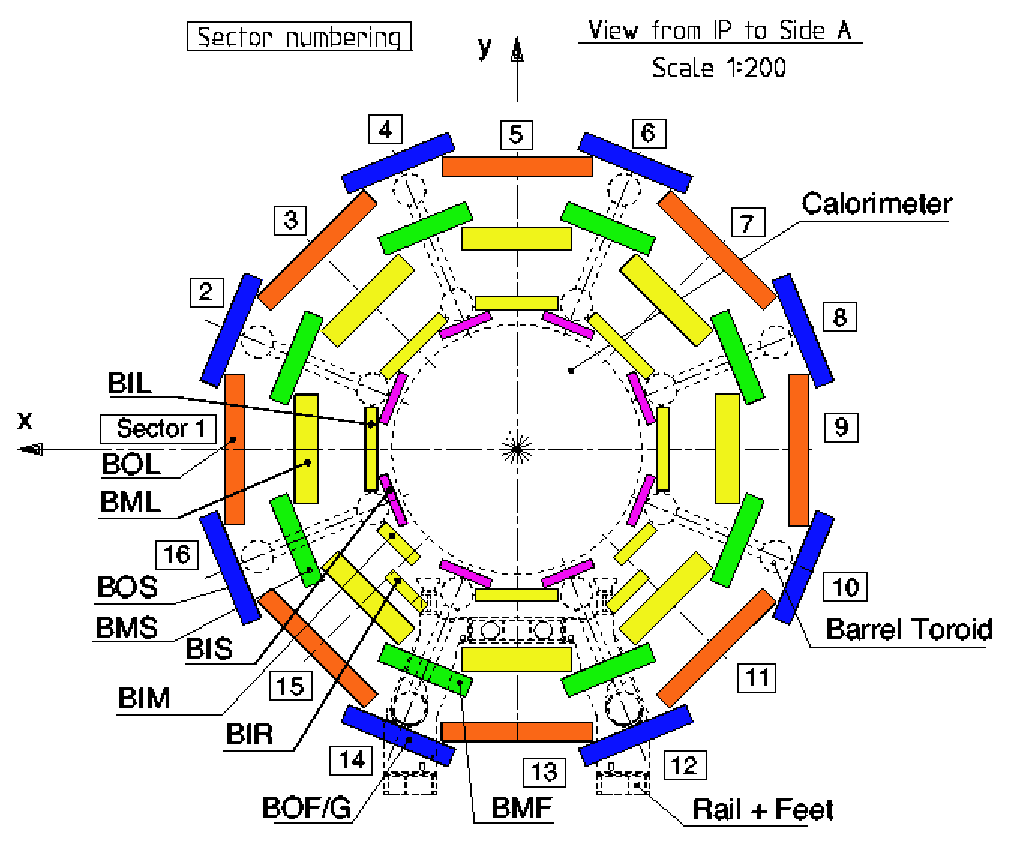
\includegraphics[width=.4\textwidth]{detector/figures/muonSect2}}
	\subfigure[]{\label{fig:muonSect}
        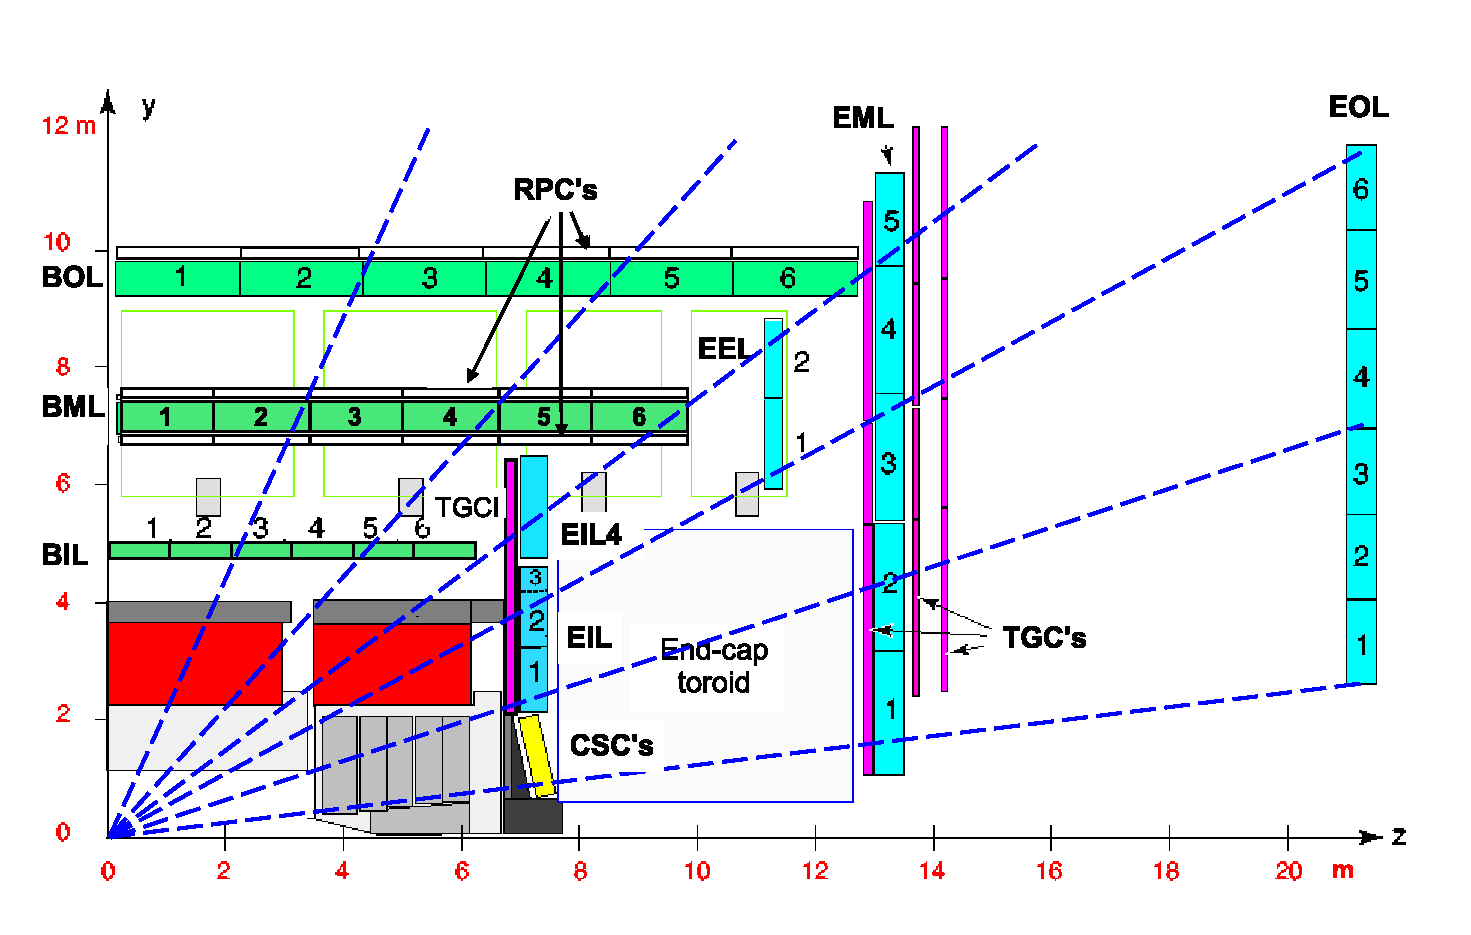
\includegraphics[width=.5\textwidth]{detector/figures/muonSect}}
	\caption{(a) Cross section of the barrel muon system. (b) Lateral section of the muon system. 
        Barrel MDTs are shown in green, end-caps MDTs in light blue, CSC in yellow, 
        TGCs in magenta, RPCs in white.%  (From \cite{Aad:JINST})
        }
\end{center}\end{figure}


\subsubsection{Detection chambers}

MDTs and CSCs are used to detect muons in the pseudorapidity regions $|\eta|<2.0$ and
$2.0<|\eta|<2.7$ respectively. MDTs are proportional chambers constituted by 
pressurised drift tubes made of aluminium with a diameter of 30~mm and lenght varying from 0.9~m to 6.2~m. 
The gas mixture in them is 93\% argon and 7\% carbon dioxyde, the anode is a 50~$\mu$m
tungsten-rhenium wire producing a radial electric field. Each chamber is composed by 
a group of six or eight tubes placed transverse to the beam axis. This number of tubes allows
for a very good track reconstruction and high reduction of the fake tracks from random 
associations of background hits, providing a resolution on position of 80 $\mu$m.
%gives a momentum  resolution $\sigma_{p_{T}}/p_{T} < 10^{-4}$~\GeV$^{-1} \cdot p_{T}$ for tracks with $p_{T} > $300~GeV.


The CSCs are used at higher $\eta$ to better cope with the higher particle flux.
They are arranged in a system of two disks with eight chambers each. Each chamber
contains four multiwire proportional chambers (the CSCs) with wires oriented in the radial direction,
spaced by 2.5~mm and in the same gas mixture of argon and carbon dioxyde as the MDTs.
The cathode strips are oriented one perpendicularly to the anode wires (and gives the precision coordinate)
and the other parallel to the wires (and gives the transverse coordinate).
The resolution provided by the interpolation between the charges induced on neighbouring cathode strips
ranges between 50 and 70 $\mu$m.

\subsubsection{Trigger chambers}

For trigger purposes detectors with faster response than drift tubes are needed\footnote{Drift-time in tubes with a diameter of 
$\mathcal{O}\sim 10$~mm can be of $\sim500$~ns, too long with respect to the 25 ns spacing of the bunch crossings.}.
MDTs and CSCs are then coupled with special layers of trigger chambers: in the barrel region, the MDT's second layer
is covered on both sides by RPCs, while MDT's third layer is covered by a RPC alternatively on the inner and outer side;
in the end–caps, TGCs cover the inner side of MDT's first and third layers. 

A RPC is a detector with a gas-gap between two resistive bakelite plates separated by 2~mm and containing
a gas mixture of C$_{2}$H$_{2}$F$_{4}$ (94.7\%), Iso-C$_{4}$H$_{10}$ (5\%) and SF$_{6}$ (0.3\%). 
RPCs measure six points per coordinate for each particle, quickly collecting the avalanches with two 
orthogonal sets of pick-up strips that provides a position resolution of 1 cm in each plane and 1 ns time resolution,
allowing for individual bunch crossing discrimination. Also RPCs provide the $\phi$ coordinate for the tracks in
the final analysis, since MDTs only give the $\eta$ coordinate.

TGCs are similar to CSCs, have 1.8~mm wire-to-wire separation and 
1.4~mm wire-to-cathode separation. They use a highly quenching gas mixture of CO$_{2}$ 55\% and n-C$_{5}$H$_{12}$ 45\%
and provide  a spatial resolution of about 1~mm and a time resolution of 5~ns.

\section{Forward sub-detectors}\label{sec:forward}

ATLAS is equipped with some detectors in the forward regions to perform additional measurements or
monitoring studies. In particular, the Minimum Bias Trigger Scintillators (MBTS), that are somehow
embedded in the structure of TileCal extended barrel modules (see Figure~\ref{fig:extendedbarrel})
and share with it the readout electronics, as they are also read by wavelenght-shifting fibers.
The MBTS consist of 32 scintillator paddles assembled in two disks covering the pseudorapidity region
$2.09<|\eta|<3.84$ and are used for trigger purposes to detect minimum bias activity during the first
runs of the LHC. 

MBTS are also used for relative luminosity measurements, but there are two detectors specifically
built to determine the luminosity delivered to ATLAS: LUCID and ALFA. LUCID (LUminosity measurements
using Cerenkov Integrating Detector) is made of 32 tubes surrounding the beam pipe 17~m
far from the interaction point on both sides of ATLAS and measures the luminosity bunch by bunch.
ALFA (Absolute Luminosity For ATLAS) is only activated during special runs, and consists of 8 
scintillating fibers detectors placed at 240~m from the interaction point inside roman pots, above and
below the beam pipe.

Another luminosity monitorer is the Zero-Degree Calorimeter, whose main purpose is to determine the centrality of heavy-ion
collisions. Placed at 140~m from the interaction point on both sides of the beam axis, is made of quartz rods
alternated with tungsten plates.

Finally, the Beam Condition Monitor (BCM) is made of two sets of diamond sensors located 184~cm close
to the interaction point along the beam and 5.5~cm close along $R$. Its task is to detect beam losses,
potentially harmful for ATLAS, and in that case to alert LHC in order to stop the accelerator.



\begin{figure}[tb]\begin{center}
	\subfigure{
  	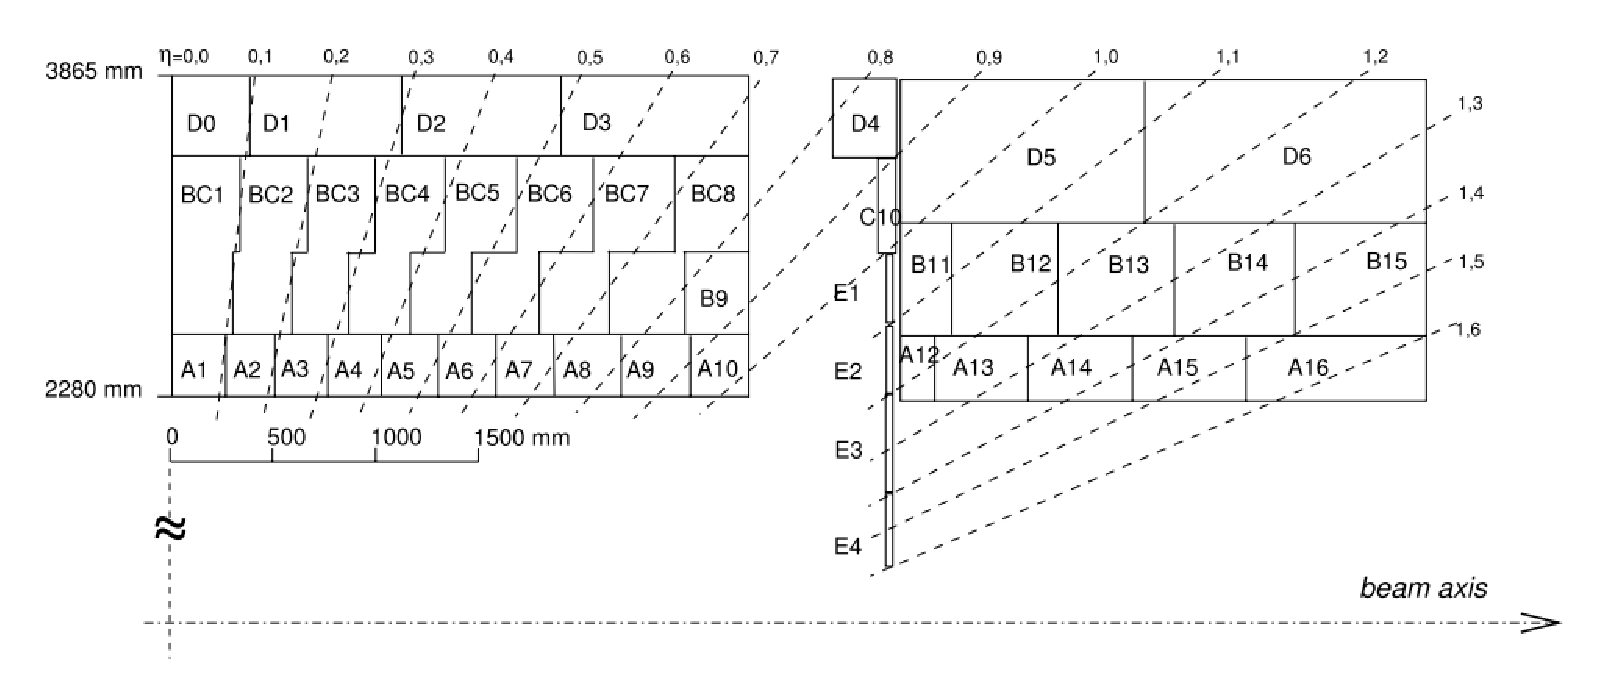
\includegraphics[width=0.\textwidth]{detector/figures/extendedbarrel}}
	\caption{Schematic of a section of TileCal barrel and extended barrel modules, with the
        cells division. The parts labelled with ``E'' are the MBTS.\label{fig:extendedbarrel}}
\end{center}\end{figure}


\section{Trigger system}\label{sec:trigger}

It was already introduced at the beginning of this Chapter the issue
faced by LHC experiments of dealing with a huge amounts of events
at very high frequencies. We remind that considering the nominal LHC
luminosity of \highL\ a rate of interactions of 40~MHz is expected!
This poses serious technical difficulties as the maximum frequency
at which data can be recorded is limited to 200~Hz considering the
limited capacity for storage.

ATLAS developed a trigger system able to reduce by a factor of 10$^6$
the amount of data to be kept by selecting only interesting physics events.
The system is divided in three levels characterized by increasing sofistication
and diminishing speed. At the very first indeed we will need a really quick and
simple criterium to reject uninteresting events. The reduced information can then be
processed with somehow slower logic by the other two High Level Triggers (HLT).
A drawing of the system is shown in Figure~\ref{fig:trigger}.

\begin{figure}[tb]\begin{center}
	\subfigure{
  	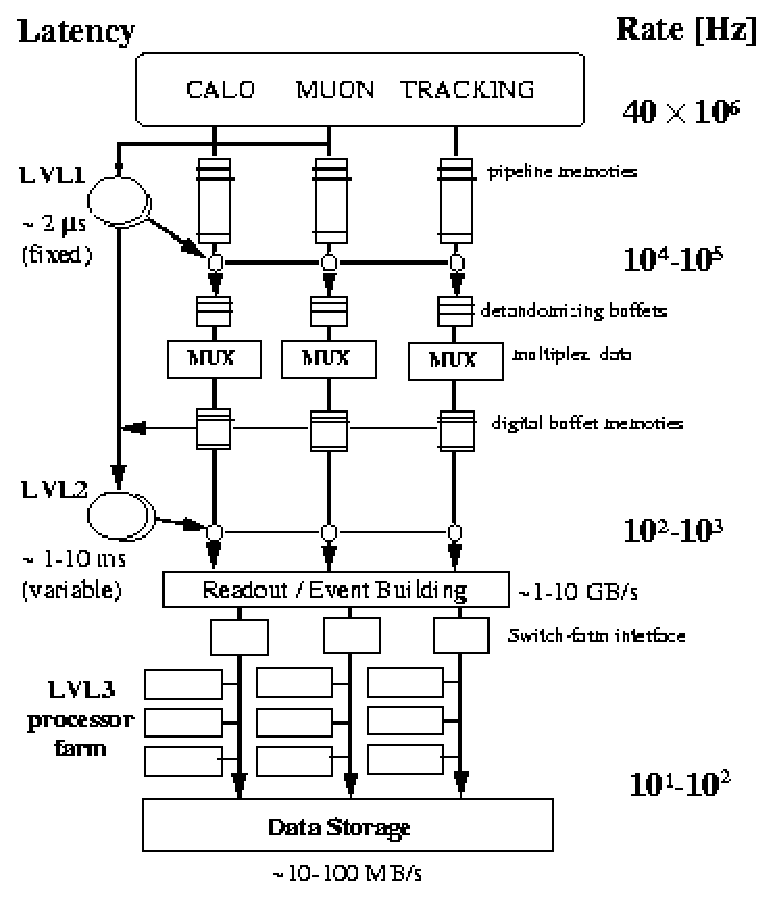
\includegraphics[width=0.5\textwidth]{detector/figures/triggerscheme}}
	\caption{Schematic drawing of the three-level trigger system of ATLAS.\label{fig:trigger}}
\end{center}\end{figure}

Most of the trigger chains used for physics are un-scaled in the
sense that all the events passing the selection are kept, but there
are also pre-scaled trigger chains that contain either too many events
or events considered not physically interesting. These trigger chains
are used for checks or calibration rather than physics analysis, and the
prescaling value $P$ means that of all the events that would have passed 
the trigger, $1/P$ were accepted.

With the term ``trigger chain'' we refer to the sequence of selections
defining a certain trigger object, with a naming convention like:
\begin{equation*}\label{eq:}
{\rm [LEVEL][N][TYPE(S)][THRESHOLD][ISOLATION][QUALITY]},
\end{equation*}
where the components, from left to right, are: the trigger level used; the
multiplicity of the type; the object candidate; the threshold applied to
the transverse momentum or energy of the object candidate; the object isolation;
the severity of the final algorithm requirements (this applies only to the Event
Filter level).

Trigger chains define a {\it trigger menu}, where they are associated to their
prescale value $P$, and which is chosen based on the physics program of the
data taking period taking into account the LHC luminosity. 

Defining the data taking period time unit as ``Luminosity Block'' (LB), typically
a few minutes of  data taking, information on beam conditions, detector performance 
and events passing any of the trigger chains of the trigger menu are stored
to be then used in the analyses. All the LB occurring between the start and the
end of a stable beam collision period compose a ``run''. Runs are finally grouped
in ``Data Periods'', labelled with capital letters (``Period A'', ``Period B'', {\it etc}.),
when they pertain to the same general detector condition, machine configuration and
trigger menu.




\subsection{Level 1 trigger}\label{sec:lvl1}

The Level 1 trigger (L1) is completely based on the hardware of the detector,
taking information from calorimeters, from the muon spectrometer trigger
systems RPC and TGC (Section~\ref{sec:muonspec}) and from the MBTS (Section~\ref{sec:forward}) 
at 40~MHz (the frequency of the beam crossing) and reducing it to 75~kHz by choosing events with high
transverse momentum or high missing transverse energy.

Using dedicated fast front-end electronics (the typical decision time being less than
2~$\mu$s), calorimeter cells are analogically 
summed to build calorimetric towers which, if having an energy higher than a 
certain threshold, will activate a trigger chain.

These trigger chains will then be combined with the information from the
muon spectrometer to form the so-called Region of Interest (RoI) that is
passed to the next trigger level.


\subsection{Level 2 trigger}\label{sec:lvl2}

Starting from the RoI, the Level 2 trigger (L2) will reduce the 75~kHz to
3.5~kHz of events with an average decision time of 40~ms. At this
stage the information from the trackers is incorporated to the RoI
to build candidate object (electrons, photons, muons) and 
better obtain its position and energy with simplified algorithms
quick enough to respect the limit on the decision time.

\subsection{Event filter}\label{sec:lvl3}

The last trigger, Level 3, is called Event Filter (EF) since
at this point the physics objects are built using the same
algorithms as the off-line reconstruction, with looser selections. With an execution time
amounting to 4~s, the EF reduces the event rate to the goal value
of 200~Hz.
Events passing the EF are assigned to {\it streams} defined to separate
the events into different datasets for different analysis interests, e.g.
electron streams, muon streams, jet streams {\it etc}.

As an example, one of the trigger chains used in our analysis is 
\texttt{EF\_mu24i\_tight}: it selects events at the EF level with one 
muon with $p_T>24$~\gev\ and some isolation requirement which passes
the muon reconstruction algorithm cuts defined as ``tight''
(more on event reconstruction is reported in the dedicated Chapter~\ref{chap:objects}).

\section{Data Quality}\label{sec:daq}

The totality of p-p collisions recorded by ATLAS, which differs from the amount
delivered by the LHC because of data-taking inefficiencies, is still
not 100\% usable by physics analyses. Indeed, every subdetector needs to
perform some routine checks %(usually done by PhD students) 
on the quality of the data they recorded in order to certify that its performace
was conform to the expectations. So-called ``Good Runs Lists'' (GRL) are
compiled stating for each LB what was ``OK'' and what not.
The single analyses will then decide which GRL to use, based on their specific
needs of the individual subsystems.


\clearpage{\pagestyle{empty}\cleardoublepage}
\clearpage{\pagestyle{empty}\cleardoublepage}

\chapter{Objects reconstruction}\label{chap:objects}

\section{Electrons}\label{sec:electrons}
\section{Muons}\label{sec:muons}
\section{Jets}\label{sec:jets}



\clearpage{\pagestyle{empty}\cleardoublepage}
\clearpage{\pagestyle{empty}\cleardoublepage}

\chapter{Monte Carlo simulation and SM background samples}\label{chap:mc}


\clearpage{\pagestyle{empty}\cleardoublepage}
\clearpage{\pagestyle{empty}\cleardoublepage}

\chapter{Searches for vector-like top partner pairs in the single lepton channel}~\label{chap:vlq}

Starting from this chapter, and continuing in Chapter~\ref{chap:wbx} 
and Chapter~\ref{chap:htx}, we are going to describe two 
searches for vector-like top partners \TTbar\ pairs performed in the single 
lepton\footnote{In the following, with the word ``lepton'' we will 
refer either to an electron or a muon, assumed to come from the leptonic
decay of a $W$ boson or a leptonic $\tau$ decay.}
%with its associated neutrino, which is considered to be the only particle contributing to the transverse missing energy \met.}
 channel. These analyses
are optimized for different final states and are thus complementary.
The analyses are performed using a partial dataset of the pp collisions at the \cme\ 
of \rts=8~\tev\ collected during 2012 at the ATLAS detector, corresponding to an integrated luminosity of  14.3~\ifb.
The first search focuses on  vector-like top partners decay channels with high 
Branching Ratio (BR) to 
a $W$ boson and a bottom quark, while the second search is optimized for events with 
high BR to a Higgs boson and a top quark.
%and is performed using the full dataset of pp collisions at the \cme\ of \rts=8~\tev\ collected during 2012 at the ATLAS detector, consinsting in 20.34~\ifb, while
%search for vector-like top partners with high BR to $Ht$
%uses a partial dataset of the same data, amounting to 14.3~\ifb.

This chapter is devoted to the presentation of the general features that are common to 
the two analyses and is organized as follows: first in Section~\ref{sec:strategy}
we review the strategy for vector-like quark searches adopted 
by the Exotics group of the ATLAS collaboration; Section~\ref{sec:presel}
summarises the common event preselection for data and few general concepts in the
analyses design; Section~\ref{sec:datasets}
describes the Monte Carlo samples used in the searches, which
are in general common to both analyses with only few exceptions that are reported,
and how the multi-jet background from QCD events is
obtained; Section~\ref{sec:systematics} introduces the general treatment of systematic uncertainties.
%The two analyses are then presented in details in Chapter~\ref{chap:wbx} 
%(\TTbar\ pairs decaying to \wbx\ ) and in Chapter~\ref{chap:htx}
%(\TTbar\ pairs decaying to \htx\ ). The final results are presented 
%in Chapter~\ref{chap:results}.

\section{General strategy for vector-like quark pairs searches}\label{sec:strategy}

The phenomenology for vector-like quarks was described already in Section~\ref{sec:THvlq}
of this dissertation. Here we will only briefly re-introduce the concepts on which
the strategy for the searches has been built. Table~\ref{tab:vlqdecays} collects the 
decay modes for vector-like quarks in the singlet and doublet models. It is evident
from the richness of the final state phase space, combined with the unpredicted mass
of the heavy objects that could span from few hundreds of \gev s (down to the values exluded by
previous searches) up to  $\sim 1$~\tev\ (since we focus on pair production of vector-like
quarks, which is favoured up to this mass scale)% as shown in Figure~\ref{fig:vlqxsec}), 
that is impossible to cover it with a single inclusive search.

\begin{table}[htb]\centering
\begin{tabular}{|lc|lc|}\toprule
\hskip2ex VLQ &  Decay & \hskip2ex VLQ  & Decay \\ 
\hskip1ex Singlets &  modes & \hskip1ex Doublets & modes\\
& & &\\
$T(+2/3)$ & $W^+b,\, Ht,\, Zt$ & \multirow{2}{*}{$\quad\bigg(\begin{array}{c}T \\ B\end{array}\bigg)$} & $W^+b,\, Ht,\, Zt$\\ 
& & & $ W^-t,\, Hb,\, Zb$\\
$B(-1/3)$ & $ W^-t,\, Hb,\, Zb$ & & \\
& & \multirow{2}{*}{$\quad\bigg(\begin{array}{c}T \\ X\end{array}\bigg)$} & $Ht,\, Zt$\\
$X(+5/3)$ & $W^+t$ & & $W^+t$\\
& & &\\
$Y(-4/3)$ & $W^-b$ & \multirow{2}{*}{$\quad\bigg(\begin{array}{c}B \\ Y\end{array}\bigg)$} & $Hb,\, Zb$\\
& & & $W^-b$\\\bottomrule
\end{tabular}
\caption{Allowed decay modes for vector-like singlets and doublets.}\label{tab:vlqdecays}
\end{table}

%\begin{figure}[htb]\begin{center}
%	\subfigure{
%  	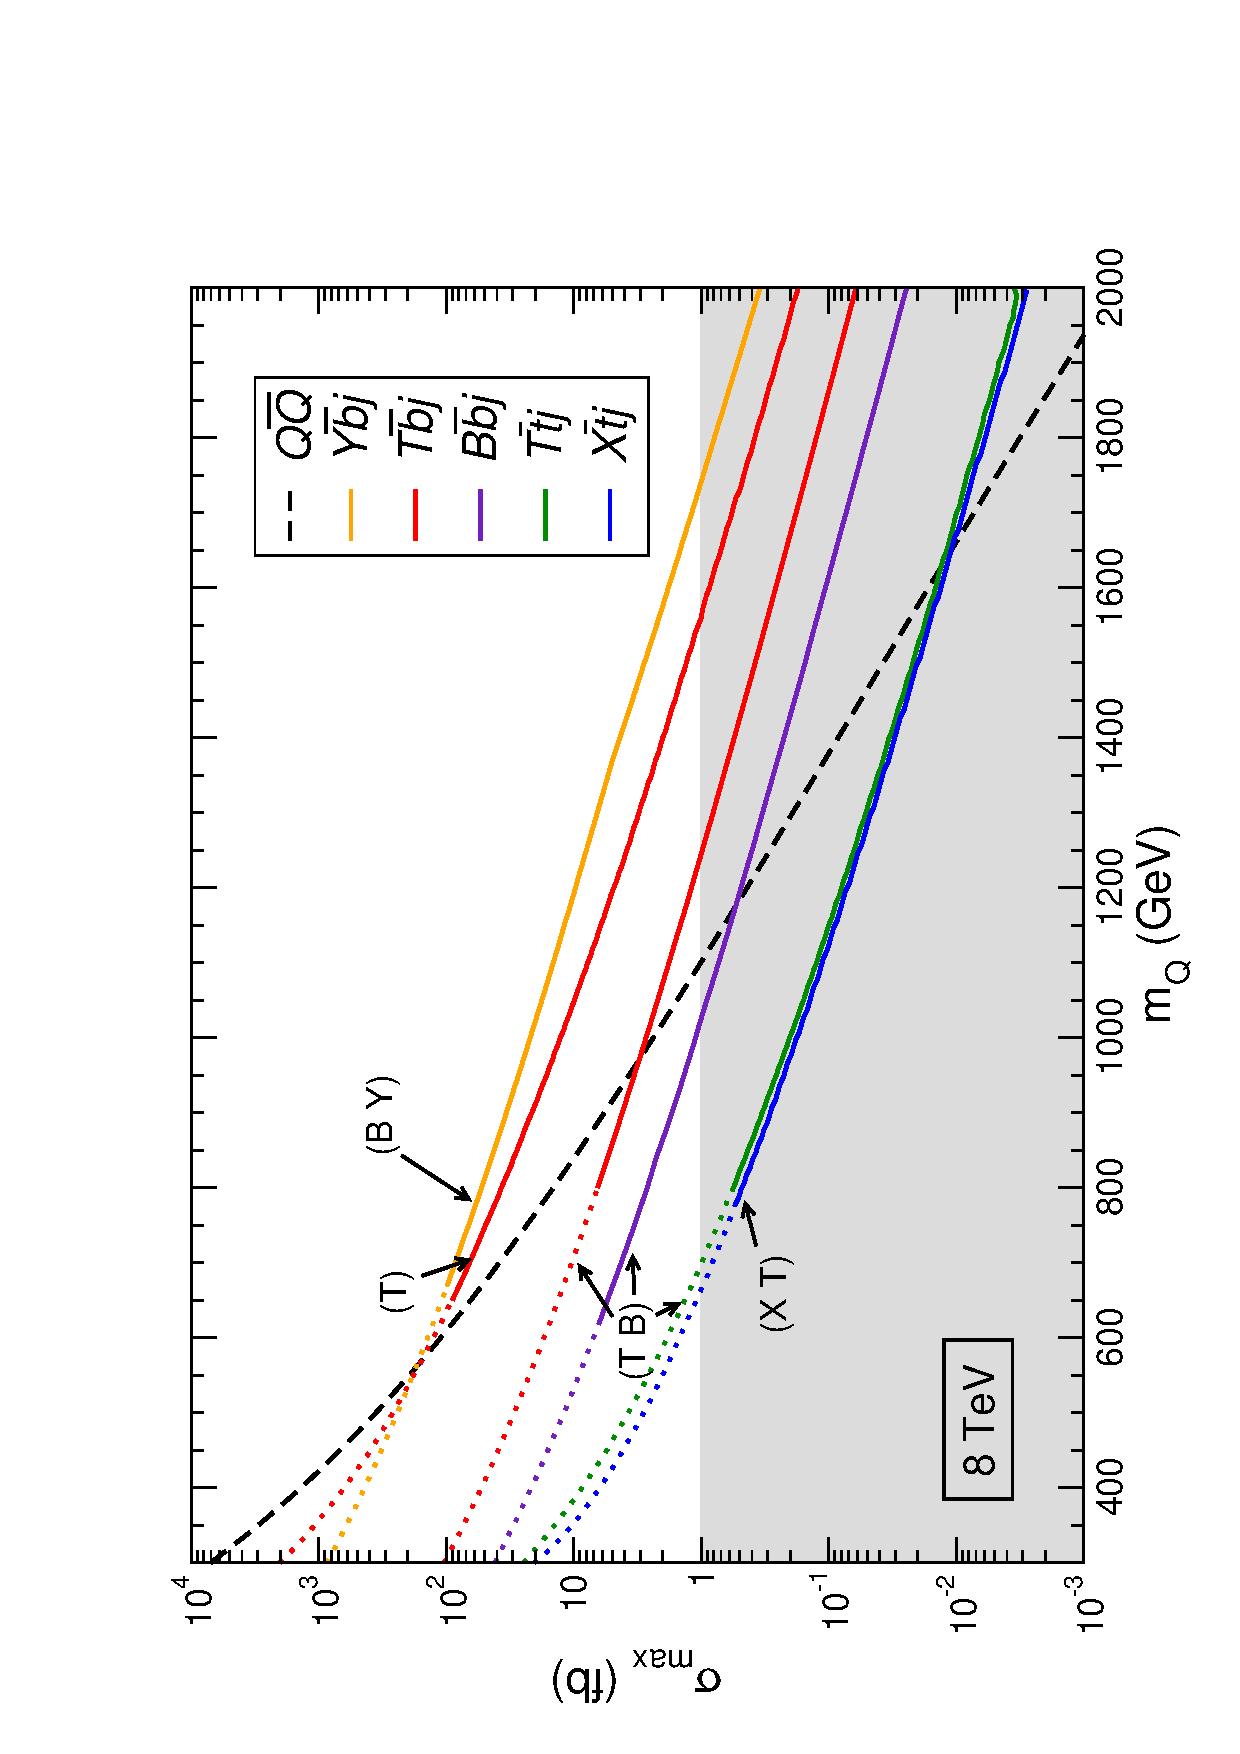
\includegraphics[width=0.65\textwidth, angle=270]{vlq_analysis/figures/xsec-8}}
%	\caption{\label{fig:vlqxsec} Pair and single production cross sections  for heavy 
%        quarks in proton-proton collisions at $\sqrt{s}=8$~TeV~\cite{Aguilar-Saavedra:2013qpa}.}
%\end{center}\end{figure}

The BR of vector-like top and bottom partners to the allowed decay modes depends
on the mass of the heavy quark and on the considered model (in our case, singlet or doublet
scenario), as shown in Figure~\ref{fig:vlqBRs}.
Each decay mode has specific features that allow to define powerful, optimized searches.
Therefore in order to exploit this opportunity and at the same time stay as model independent
as possible, different searches for vector-like quarks are performed at ATLAS
to be later combined, each of them sensitive to specific channels.
To ensure a comprehensive coverage of the phase space, a two-dimensional plane is defined 
(Figure~\ref{fig:2dplane}) as follows:
along the Y axes is the BR of the decay 
modes with a Higgs boson in the final state; along the X axis is the BR 
of the decay modes with a $W$ boson in the final state.
The BR to the channel with a $Z$ boson in the final state is then fixed by the 
unitarity requirement BR($T/B\to  Zt/b$) = 1 - BR($T/B\to Ht/b$) - BR($T/B\to Wb/t$).
A plane of this kind is defined for every vector-like quark mass point considered 
in the analysis. Each point of each plane therefore represents a 
uniquely defined model, and analyses are performed for every configuration
to either find deviations from expectations or to set a 95\% Confidence Level (CL) exclusion.
The final objective of the joint strategy is to cover the full plane by combining
analyses probing the different signatures.

\begin{figure}[h!tb]\begin{center}
	\subfigure[]{\label{fig:vltBRs}
  	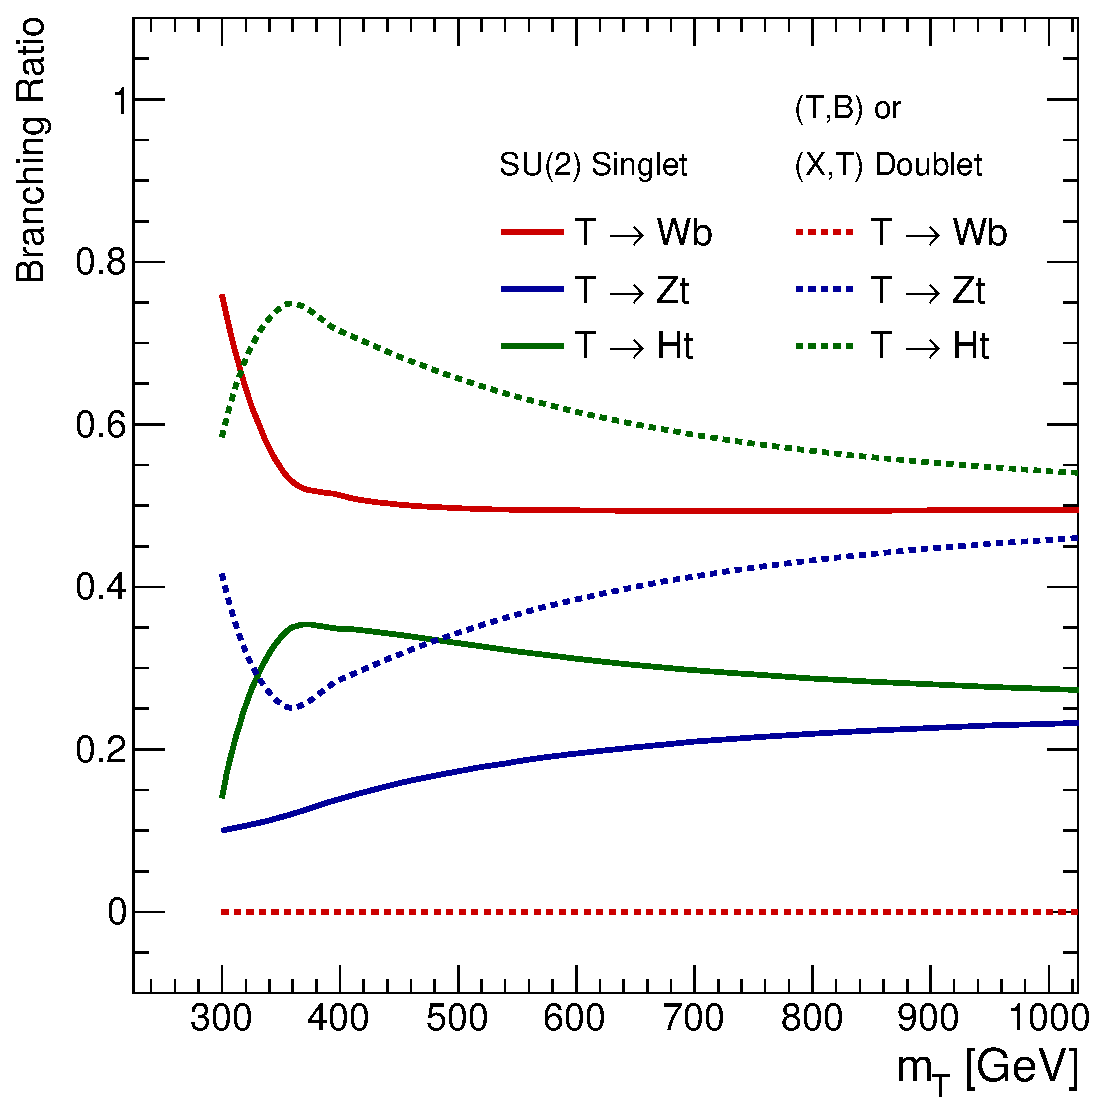
\includegraphics[width=0.47\textwidth]{vlq_analysis/figures/fig_02a.eps}}
	\subfigure[]{\label{fig:vlbBRs}
  	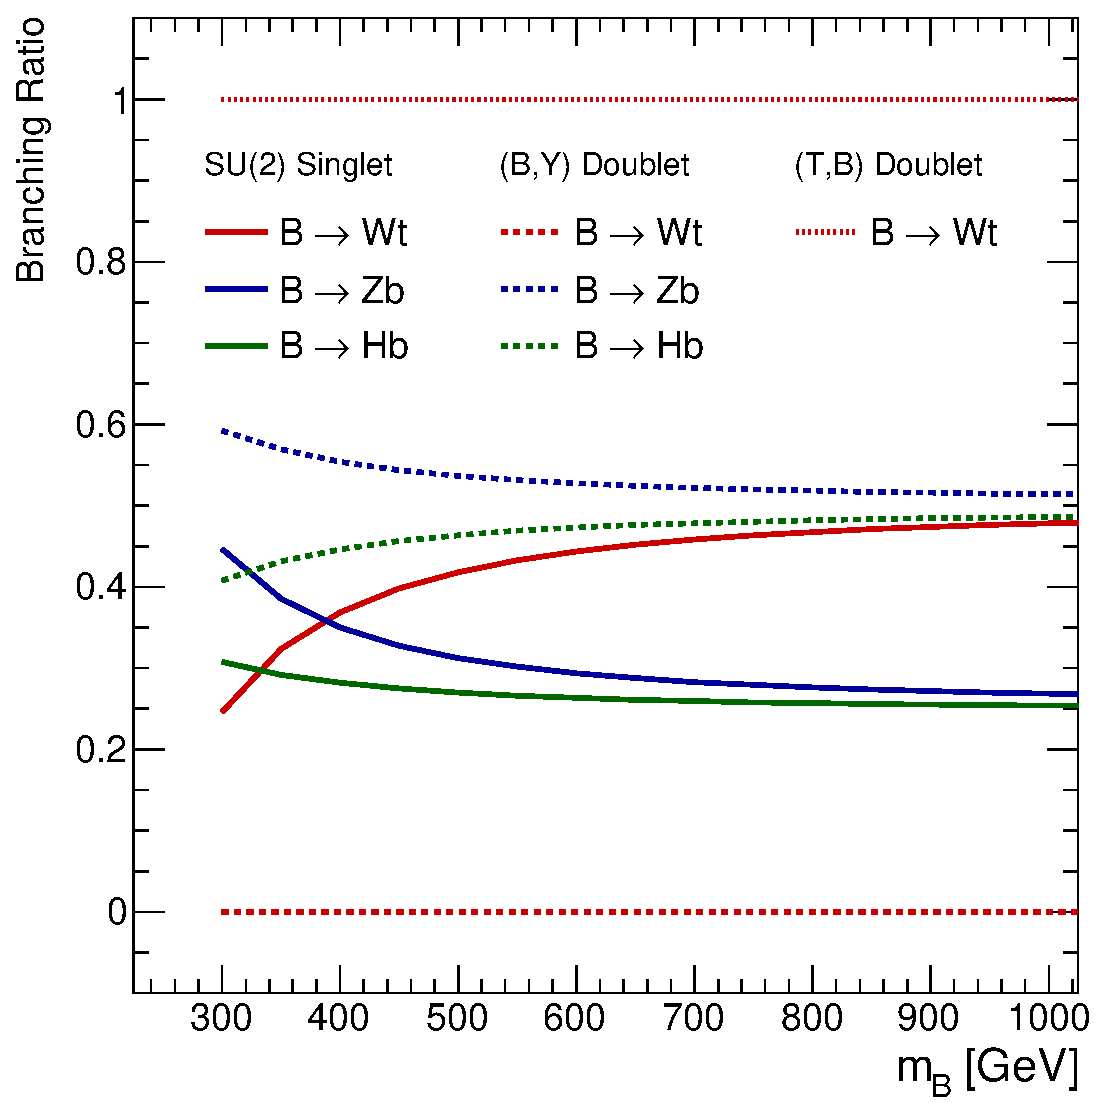
\includegraphics[width=0.47\textwidth]{vlq_analysis/figures/fig_02b.eps}}
	\caption{Branching ratio of vector-like top (a) and bottom (b) partners as a function of the heavy quark mass $m_T$ and $m_B$ respectively~\cite{ATLAS-CONF-2013-056} for singlet and doublet models.\label{fig:vlqBRs}}
\end{center}\end{figure}

\begin{figure}[h!bt]\begin{center}
	\subfigure{
        \begin{pgfpicture}{0.0\textwidth}{0.0\textheight}{.5\textwidth}{.5\textwidth}
%\begin{pgfpicture}{0.0\textwidth}{0.0\textheight}{1.\textwidth}{.6\textwidth}

\begin{pgfscope}
\pgfsetendarrow{\pgfarrowlargepointed{6pt}}
\pgfsetlinewidth{1.5pt}

\begin{pgftranslate}{\pgfpoint{0.05\textwidth}{0.05\textheight}}
%\begin{pgftranslate}{\pgfpoint{0.1\textwidth}{0.15\textheight}}
  {
    %\color{black}
    \color{black!50!red}
    \pgfputat{\pgfxy(3.5,-0.5)}{\pgfbox[left,base]{BR($T\to Wb$)}}
  }
  {
    \color{black!50!blue}
    \pgfputat{\pgfxy(3.5,-0.8)}{\pgfbox[left,base]{BR($B\to Wt$)}}
  }
  {
    \begin{pgfrotateby}{\pgfdegree{90}}
      {
        \color{black!50!red}
        \pgfputat{\pgfxy(3.5,0.4)}{\pgfbox[left,base]{BR($T\to Ht$)}}
      }
      {
        \color{black!50!blue}
        \pgfputat{\pgfxy(3.5,0.7)}{\pgfbox[left,base]{BR($B\to Hb$)}}
      }
    \end{pgfrotateby}
  }
  {
    \pgfsetlinewidth{1.5pt}
    \color{gray!30!white}%\color{light-gray}
    \pgfmoveto{\pgfxy(5,0)}
    \pgflineto{\pgfxy(5,5)}
    \pgflineto{\pgfxy(0,5)}
    %\pgfstroke
    \pgffill
  }
  {
    %\color{black}
    \pgfputlabelrotated{0.5}{\pgfxy(0,5)}{\pgfxy(5,0)}{8pt}{\pgfbox[center,base]{Forbidden}}
  }
  \begin{pgfscope}
    \pgfmoveto{\pgfxy(5,0)}
    \pgflineto{\pgfxy(0,0)}
    \pgflineto{\pgfxy(0,5)}
    {
      \color{yellow!30!white}
      \pgfclip
      \pgfcircle[fill]{\pgfxy(.5,4)}{35pt}
    }
    {
      \pgfputat{\pgfxy(0.15,3.6)}{\pgfbox[left,base]{\large{\color{black!70!red}$Ht$}{\color{black!70!blue}$(b)$}}}
    }
    {
      \color{yellow!30!white}
      \pgfcircle[fill]{\pgfxy(.6,.6)}{35pt}
    }
    {
      \pgfputat{\pgfxy(0.15,.4)}{\pgfbox[left,base]{\large{\color{black!70!red}$Zt$}{\color{black!70!blue}$(b)$}}}
    }
    {
      \color{yellow!30!white}%\color{light-gray}
      \pgfcircle[fill]{\pgfxy(4,0)}{35pt}
    }
    {
      \pgfputat{\pgfxy(3.2,0.4)}{\pgfbox[left,base]{\large{\color{black!70!red}$Wb$}{\color{black!70!blue}$(t)$}}}
    }
  \end{pgfscope}
  {
    %\color{black}
    \pgfsetendarrow{\pgfarrowlargepointed{6pt}}
    \pgfsetlinewidth{1.5pt}
    \pgfline{\pgfxy(0,0)}{\pgfxy(5.5,0)}
    \pgfstroke
    %\pgfsetendarrow{\pgfarrowlargepointed{6pt}}
    %\pgfsetlinewidth{1.5pt}
    \pgfline{\pgfxy(0,0)}{\pgfxy(0,5.5)}
    \pgfstroke
  }

\end{pgftranslate}
\end{pgfscope}
\end{pgfpicture}
}
       	\caption{Two dimensional plane used to represend the comprehensive scan of model mixing. Searches 
        with a Higgs boson in the final state cover the top left corner; searches with a $Z$ boson in the 
        final state cover the bottom left corner; searches with a $W$ boson in the final state cover the 
        bottom right corner. The shaded area labelled as ``forbidden'' is the unphysical region where
        BR($T/B\to Ht/b$) + BR($T/B\to Wb/t$) + BR($T/B\to  Zt/b$) $>1$ \label{fig:2dplane}}
\end{center}\end{figure}


Up to the date of the writing of this dissertation, four complementary 
and quasi model-independent analyses have been performed by the Exotics working
group on the partial dataset of 14.3~\ifb\ of proton-proton collision data at 
$\sqrt{s}=8\tev$.  
Two analyses investigated dilepton channels and two probed single lepton channels.

The search for vector-like bottom and top partners in the same-sign 
dilepton channel~\cite{ATLAS-CONF-2013-051}
investigates a channel
with very small contamination from Standard Model backgrounds and
is also sensitive to four-top production $pp\to t\bar{t}t\bar{t}$, 
either through the Standard Model process or a beyond-SM source such as 
pair production of scalar color-octets (sgluons) or gluinos, with subsequent 
decays to top quark pairs.
The approach of this search is to select via restrictive cuts (that also
impose a veto on a $Z\to l\bar{l}$ boson) the eventual signal
and compare the final counts with the expected yields from background sources.
Figure~\ref{fig:feyndSS} shows how the decays of vector-like bottom and top partner
pairs can contribute to the same-sign dilepton signature. From this it is easy to
understand that this search will be mainly covering the bottom right corner
of the \BBbar\ two dimensional plane of Figure~\ref{fig:2dplane} and the top 
left corner of the same plane for \TTbar.
%Data-driven techniques are used to evaluate the background contribution to the signal region coming from charge misidentification and fakes, the two main sources of background. In the end 3, 10 and 2 events are observed in the $ee$, $e\mu$ and $\mu\mu$ channels respectively. The observed counts are consistent with the expected yields in the $ee$ and $\mu\mu$ channel. A small excess of events is observed in the $e\mu$ channel, leading to a slightly weaker limit than expected, but still within a $\pm1\sigma$ band.
%These counts are consistent with the expected yields, except for the  $e\mu$ channel.

\begin{figure}[hbt]
\begin{center}
        \myskip\begin{fmffile}{fmfssBBTT}
\unitlength=1mm
\hskip-5ex
\subfigure[]{\label{fig:feyndSSBB}
    \begin{fmfgraph*}(60,30)
      \fmfleft{i1,i2}
      \fmfright{o1,o2,o3,o4,o5,o6,o7,o8}
      \fmflabel{$g$}{i1}
      \fmflabel{$g$}{i2}
      %\fmflabel{$b$}{}
      %%%%
      \fmf{phantom}{o1,v4,v3,v2,v1,i1}
      \fmf{phantom}{o2,v4,v3,v2,v1,i1}
      \fmf{phantom}{o3,v5,v3,v2,v1,i1}
      \fmf{phantom}{o4,v5,v3,v2,v1,i1}
      %%%%
      \fmf{phantom}{o5,v7,v6,v2,v1,i2}
      \fmf{phantom}{o6,v7,v6,v2,v1,i2}
      \fmf{phantom}{o7,v8,v6,v2,v1,i2}
      \fmf{phantom}{o8,v8,v6,v2,v1,i2}
      %%%%
      \fmflabel{$\bar{b}$}{o1}
      \fmflabel{\textcolor{red}{$W^{-}$}}{o2}
      \fmflabel{\textcolor{blue}{$W^{+}$}}{o4}
      \fmflabel{\textcolor{red}{$W^{-}$}}{o8}
      \fmflabel{\textcolor{blue}{$W^{+}$}}{o6}
      \fmflabel{$b$}{o5} 
      \fmf{plain}{o1,v4}
      \fmf{photon}{o2,v4}
      %%
      \fmf{photon}{o4,v3}
      \fmf{plain}{o5,v7}
      \fmf{photon}{o6,v7}
      \fmf{photon}{o8,v6}
      %%%
      \fmf{plain,label=$\bar{B}$}{v2,v3}
      \fmf{plain,label=$B$}{v2,v6}
      \fmf{plain,label=$\bar{t}$,l.dist=-7thick}{v4,v3}
      \fmf{plain,label=$t$}{v7,v6}
      \fmf{curly}{i1,v1}
      \fmf{curly}{i2,v1}
      \fmf{curly,label=$g$,l.dist=-7thick}{v1,v2}
    \end{fmfgraph*}
}\hskip5ex
\subfigure[]{\label{fig:feyndSSTT}
    \begin{fmfgraph*}(60,30)
      \fmfleft{i1,i2}
      \fmfright{o1,o2,o3,o4,o5,o6,o7,o8}
      \fmflabel{$g$}{i1}
      \fmflabel{$g$}{i2}
      %\fmflabel{$b$}{}
      %%%%
      \fmf{phantom}{o1,v4,v3,v2,v1,i1}
      \fmf{phantom}{o2,v4,v3,v2,v1,i1}
      \fmf{phantom}{o3,v5,v3,v2,v1,i1}
      \fmf{phantom}{o4,v5,v3,v2,v1,i1}
      %%%%
      \fmf{phantom}{o5,v7,v6,v2,v1,i2}
      \fmf{phantom}{o6,v7,v6,v2,v1,i2}
      \fmf{phantom}{o7,v8,v6,v2,v1,i2}
      \fmf{phantom}{o8,v8,v6,v2,v1,i2}
      %%%%
      \fmflabel{\textcolor{red}{$\bar{t}, \bar{t}$}$, \bar{b}$}{o1}
      \fmflabel{$Z, H,$ \textcolor{red}{$W^-$}}{o3}
      \fmflabel{$\bar{b}$}{o7}
      %\fmflabel{\textcolor{red}{$W^{-}$}}{o2}
      \fmflabel{\textcolor{blue}{$W^{+}$}}{o8}
      \fmflabel{\textcolor{red}{$W^{-}$}}{o5}
      \fmflabel{\textcolor{blue}{$W^{+}$}}{o6}
      %\fmflabel{}{o5} 
      \fmf{plain}{o1,v4}
      \fmf{photon}{o3,v4}
      %%
      %\fmf{photon}{o4,v3}
      \fmf{photon}{o5,v7}
      \fmf{photon}{o6,v7}
      \fmf{plain}{o7,v8}
      \fmf{photon}{o8,v8}
      %%%
      \fmf{plain,label=$\bar{T}$,l.dist=-6thick}{v2,v4}
      \fmf{plain,label=$T$}{v2,v6}
      %\fmf{plain,label=$\bar{t}$,l.dist=-7thick}{v4,v3}
      \fmf{plain,label=$t$}{v6,v8}
      \fmf{dashes,label=$H$,l.dist=-6thick}{v7,v6}
      \fmf{curly}{i1,v1}
      \fmf{curly}{i2,v1}
      \fmf{curly,label=$g$,l.dist=-7thick}{v1,v2}
    \end{fmfgraph*}
}
\end{fmffile}
\myskip
	\caption{Feynman diagrams for \BBbar\ (left) and \TTbar\ (right)
        decays that can result in a final state with two same-sign leptons,
        in the case that the same-sign $W$ bosons (highlighted in different colors;
        on the right the anti-top quarks associated to the $Z$ or Higgs bosons are
        also highlighted as they will originate a $W^{-}$ boson) decay
        into a lepton and a neutrino. \label{fig:feyndSS}}
\end{center}
\end{figure}


The search in the opposite-charge dilepton channel~\cite{ATLAS-CONF-2013-056} 
focuses on vector-like bottom  (top) partners decay channels where at least one 
heavy quark decays into a $Z$ boson and a bottom (top) quark. 
Here the strategy is to reconstruct the $Z$ boson from the opposite-charge lepton
pair and use the invariant mass of the $Z$ boson candidate paired  with the highest 
$p_T$ $b$-jet as final discriminant variable to perform the statistical analysis.
It is then straight-forward to expect this search to efficiently cover the bottom
left corners of both the \BBbar\  and \TTbar\  two dimensional planes of
Figure~\ref{fig:2dplane}.


The searches in the single lepton channel are focused on vector-like top partner
pairs decays and are optimized for two distinctive signatures. One search
exploits the boosted kinematics of the $W$ boson from vector-like top partners decays
to reconstruct it from its hadronic channel final state 
particles~\cite{ATLAS-CONF-2013-060}. The heavy quark invariant mass is 
then reconstructed pairing the boosted  $W$ boson  with a \bjet\ and this
distribution is used to perform the statistical analysis. It is evident that this
search is going to cover the bottom right corner of the \TTbar\  two dimensional plane 
of Figure~\ref{fig:2dplane}.

The other search in the single lepton channel considers final states with high
jet and \bjet\ multiplicities as a result of the decay of at least one heavy quark
into a Higgs boson (assumed to decay into \bbbar) and a top 
quark~\cite{ATLAS-CONF-2013-018} (see Figure~\ref{fig:feyndHTX}). The distribution
of the  total transverse momentum of the event is then used to perform the statistical 
analysis. This search is mainly sensitive to the top left corner of the \TTbar\  
two dimensional plane of Figure~\ref{fig:2dplane}.


\begin{figure}[hbt]
\begin{center}
        \myskip\begin{fmffile}{fmfTThtx}
\unitlength=1mm
\begin{fmfgraph*}(60,50)
  \fmfleft{i1,i2,i3,i4,i5,i6,i7,i8}
  \fmfright{o1,o2,o3,o4,o5,o6,o7,o8}
  \fmflabel{$g$}{i3}
  \fmflabel{$g$}{i6}
  %\fmflabel{$b$}{}
%%%%
  \fmf{phantom}{i1,v11,v12,v13,v14,o1}
  \fmf{phantom}{i2,v21,v22,v23,v24,o2}
  \fmf{phantom}{i3,v31,v32,v33,v34,o3}
  \fmf{phantom}{i4,v41,v42,v43,v44,o4}
  \fmf{phantom}{i5,v51,v52,v53,v54,o5}
  \fmf{phantom}{i6,v61,v62,v63,v64,o6}
  \fmf{phantom}{i7,v71,v72,v73,v74,o7}
  \fmf{phantom}{i8,v81,v82,v83,v84,o8}
  \fmffreeze
  \fmflabel{$\bar{t}, \bar{t}, \bar{b}$}{o1}
  \fmflabel{$Z, H, W^-$}{o3}
  \fmf{plain}{o1,v32}
  \fmf{photon}{o3,v32}
  \fmf{plain,label=$t$}{v62,v73}
  \fmflabel{$b$}{o6}
  \fmf{photon,label=$W^+$}{v74,v73}
  \fmf{plain}{o8,v74,o7}
  \fmflabel{$l^+$}{o8}
  \fmflabel{$\bar{\nu}_l$}{o7}
  \fmf{plain}{o6,v73}

  \fmf{dashes,label=$H$}{v62,v53}
  \fmf{plain}{o5,v53,o4}
  \fmflabel{$b$}{o5}
  \fmflabel{$\bar{b}$}{o4}
  %\fmf{photon,label=$H$}{v10,v11}
  %\fmf{plain}{v9,v10,v12}
  %\fmflabel{$b$}{v9}
  %\fmflabel{$\bar{b}$}{v12}
  \fmf{plain,label=$T$}{v62,v61}
  \fmf{plain,label=$\bar{T}$}{v32,v31}
  \fmf{curly}{i3,v31}
  \fmf{curly}{i6,v61}
  \fmf{plain}{v31,v61}
\end{fmfgraph*}
\end{fmffile}
\myskip
	\caption{Feynman diagrams for the $\TTbar\to Ht+X$
        decay entering the high jet and \bjet\ multiplicity final states.
        Assuming the single lepton condition, in this picture all the bosons 
        produced in the $\Tbar$ decay will decay hadronically.\label{fig:feyndHTX}}
\end{center}
\end{figure}



We will in the following treat in details the two searches for vector-like 
top partners performed in the single lepton channels, starting with the
discussion of the common features between the two analyses.


\section{Data sample and common event preselection}\label{sec:presel}

The data from pp collision events recorded at the ATLAS experiment during
2012 at a \cme\ of $\rts=8\tev$ are considered. Physics object definitions 
were discussed in Chapter~\ref{chap:objects}.
Events collected during
stable beam periods are required to pass data quality requirements and
single lepton trigger selection. In order to maximize trigger
efficiency, different transverse momentum threshold triggers are combined
through a logical \OR, with the lower \pt\ ones including isolation requirements
that result in inefficiencies for high \pt\ lepton candidates, recovered with
the use of the higher threshold triggers. The electron triggers have
\pt\ thresholds of 24 and 60~\gev, the muon ones of 24 and 36~\gev\ (Section~\ref{sec:REQtrigger}).

After passing trigger requirements, events with more than one lepton are
discarded. In addition, the only lepton of the event has to match within $\dr<0.15$ the
triggered one. As basic preselection, four jets satisfying the conditions
described in Section~\ref{sec:jets} are required, at least one of them
being tagged as a \bjet.

In order to suppress the multi-jet background from QCD processes,
combined cuts on the \met\ and on the tranverse mass of the 
leptonically decaying $W$ boson \mt\footnote{$\mt = \sqrt{2 p^\ell_{\rm T} \met (1-\cos\Delta\phi)}$, with
$p^\ell_{\rm T}$  being the transverse momentum (energy) of the muon (electron) and $\Delta\phi$ the
azimuthal angle separation between the lepton and the direction of
the missing transverse momentum.}\ 
are defined: $\met>20~\gev$ and $\met+\mt>60~\gev$.

At this point, a simple consideration about the typical expected jet
(and \bjet) multiplicity based on counting the parton multiplicities and their 
flavor is made so as to define an orthogonality
cut between the two analyses. Table~\ref{tab:jetmult} shows the 
number of jets (\bjet s) per decay channel combinations of \TTbar\ pairs, 
in the case of single lepton selection with at least four jets
(i.e. one $W$ boson will always decay into lepton and neutrino,
and $Z$ boson decay to neutrinos is excluded in the $WbZt$ channel) and assuming that
the Higgs boson decays to a bottom quark-antiquark pair.
To avoid overlap between selected events from the two analyses, in the
\wbx\ analysis events with $\geq$6 jets and $\geq$3 \bjet s are 
rejected\footnote{As will be explained later in Section~\ref{sec:htxEVT}, another orthogonality
cut will be applied in the low \bjet\ multiplicity channel of the \htx\ analysis.}.

\begin{table}\centering
\begin{tabular}{lccc}\toprule
& $Wb$ & $Ht$ & $Zt$ \\\midrule
&\cellcolor{lightgray} & & \cellcolor{lightgray}\\
\multirow{-2}{*}{$Wb$} & 
\cellcolor{lightgray}\multirow{-2}{*}{\bf 4 (2)} & 
\multirow{-2}{*}{6 (4)} & 
\cellcolor{lightgray}\multirow{-2}{*}{{\bf 6} ({\bf2}/4)} \\
\multirow{2}{*}{$Ht$} & 
\multirow{2}{*}{6 (4)} & 
\multirow{2}{*}{8 (6)} & max: 8 (4/6)\\
& & & \cellcolor{lightgray}min: {\bf6 (2)}\\
\multirow{2}{*}{$Zt$} & 
\cellcolor{lightgray}& max: 8 (4/6) & 
\cellcolor{lightgray}max: {\bf8} ({\bf2}/6) \\
& \cellcolor{lightgray}\multirow{-2}{*}{\bf6 (2/4)} & 
\cellcolor{lightgray}min: {\bf6 (2)} & 
\cellcolor{lightgray}min: {\bf6} ({\bf2}/4)\\
\bottomrule\end{tabular}\caption{Jets (\bjet s) multiplicities in 
the various possible final states. $Z$ boson decays 55\% hadronically, 
15\% of the times into \bbbar, therefore the min/max number of \bjet s 
is reported. Highlighted in bold characters are the channels that after the orthogonality 
cut will contribute to the \wbx\ analysis.}\label{tab:jetmult}
\end{table}




\section{Background and signal modeling}\label{sec:datasets}

All samples are enterely modeled using Monte Carlo simulation with the exception
of QCD multi-jet events, which are derived using data-driven techniques, and 
background from $W$ boson production in association with jets, which is obtained
from Monte Carlo at first but then is normalized to data.

The main background for both analyses is $t\bar{t}$ 
production in association with jets ($t\bar{t}$+jets)
and different choices for the generator are made
in the analyses because of the specific needs of having well
modeled regions.
In the case of the $t\bar{t}$+jets background prediction for the \htx\ analysis 
further corrections to match the data are applied, due to a mismodeling in the
heavy- and light-flavour content of the simulated sample 
(see Section~\ref{sec:htxEVT}).

$W$ boson production  in association with jets ($W$+jets) 
and QCD multi-jet events also contributes, the latter
entering into the event selection via the misidentification of a jet or a photon as an
electron or the presence of a non-prompt lepton from, e.g., semileptonic $b$- or $c$-hadron decay.
Small background contributions originate from single top quark, $Z$+jets, diboson
($WW,WZ,ZZ$), and associated $t\bar{t}V$ ($V=W,Z$) and $t\bar{t}H$ production.

\subsection{Monte Carlo simulated samples}\label{sec:MCbkg}

%All event generators using {\tt HERWIG}~\cite{HERWIG} are also interfaced to {\tt JIMMY v4.31}~\cite{jimmy} to simulate the underlying event.  
With the exception of the 
signal samples, all simulated 
samples utilise {\tt PHOTOS 2.15}~\cite{PhotosPaper} to model
photon radiation and {\tt TAUOLA 1.20}~\cite{TauolaPaper} to model
$\tau$ decays.  

All simulated samples include multiple pp
interactions and make use of the  {\tt GEANT4}~\cite{geant}
detector geometry and response simulation~\cite{atlas_sim}
with the exception of the signal samples, for which a fast simulation of
the calorimeter response is used.

All simulated samples are then processed through the same reconstruction 
software as the data and are reweighted to match 
the instantaneous luminosity profile in data. For more details
on the Monte Carlo simulation chain we refer the reader to
Chapter~\ref{chap:mc} and in particular to Section~\ref{sec:generators}.

%Additional corrections are applied so that the 
%object identification efficiencies, energy
%scales and energy resolutions match those determined in data control
%samples.


\subsubsection{$t\bar{t}$ MC@NLO}\label{subsec:MC@NLO}
Simulated samples of $t\bar{t}$ pair production  in association with jets 
($t\bar{t}$+jets or simply $t\bar{t}$ in the following)
are generated with {\tt MC@NLO} v4.01~\cite{mcatnlo_1,mcatnlo_2,mcatnlo_3} using the {\tt CT10} set of parton distribution functions (PDFs)~\cite{ct10},
with the parton-shower and fragmentation steps being performed by 
{\tt HERWIG} v6.520~\cite{HERWIG}.
The top quark mass is assumed to be equal to $172.5\gev$ and 
the samples are normalized to approximate next-to-next-to-leading-order 
(NNLO) theoretical cross section~\cite{ttbarxs}; the cross section used 
has been computed with {\tt HATHOR 1.2}~\cite{ttbarxs} using the {\tt MSTW2008}
NNLO PDF set~\cite{Martin:2009iq} and is $\sigma_{t\bar{t}}= 238^{+22}_{-24}$~pb, 
where the total uncertainty results from the sum in quadrature of the 
scale and PDF+$\alpha_S$ uncertainties according to 
the {\tt MSTW} prescription~\cite{mstw2}. 
This is the $t\bar{t}$ used in the \wbx\ analysis.

\subsubsection{$t\bar{t}$ Alpgen}\label{subsec:alpgen}
Simulated samples of $t\bar{t}$+jets are generated using
%and $W/Z$+jets events are generated using
the {\tt ALPGEN v2.13}~\cite{ALPGEN} leading-order (LO) generator and the 
{\tt CTEQ6L1} PDF set~\cite{cteq6}, with parton shower and fragmentation  
modelled through {\tt HERWIG} v6.520~\cite{HERWIG}.

A parton-jet matching scheme called ``MLM matching''~\cite{mlm} is used
in orderd to avoid double-counting  of partonic configurations
eventually generated both at the matrix-element calculation level
and at the parton-shower evolution step.

Separate samples are generated for $t\bar{t}$+light jets ($t\bar{t}$+light 
or $t\bar{t}$+LF in the following, from ``light flavour'') 
with up to three additional light partons ($u$, $d$, $s$ quarks or gluons),
and for $t\bar{t}$+heavy-flavour jets ($t\bar{t}$+HF in the following), 
including $t\bar{t}b\bar{b}$ and
$t\bar{t}c\bar{c}$.  
An algorithm based on the angular separation
between the extra heavy quarks is used to remove 
the overlap between $t\bar{t}q\bar{q}$ ($q=b,c$) 
generated from the matrix element calculation and 
from parton-shower evolution in the  $t\bar{t}$+light samples
is employed: matrix-element prediction is chosen over the parton-shower one
when $\Delta R(q,\bar{q})>0.4$, else vice-versa.

%The algorithm used is implemented in the HFOR tool~\cite{hfor}.

Again a top quark mass of $172.5\gev$ is assumed, and normalisation to the
NNLO theoretical cross section is used (see~\ref{subsec:MC@NLO})

\subsubsection{$W/Z$+jets}

Simulated samples of $W/Z$ boson production in association with jets
($W/Z$+jets in the following) are generated with up to five additional 
partons using the {\tt ALPGEN v2.13}~\cite{ALPGEN} LO generator and the 
{\tt CTEQ6L1} PDF set~\cite{cteq6}, interfaced to {\tt HERWIG} v6.520 
for parton showering and fragmentation.
The MLM matching scheme is used also here to avoid double-counting of partonic configurations 
between  matrix-element  calculation and parton showering.

The $W$+jets samples are generated separately for $W$+light jets, 
$Wb\bar{b}$+jets, $Wc\bar{c}$+jets, and $Wc$+jets, 
with the relative contributions normalized using the fraction 
of $b$-tagged jets in $W$+1-jet and $W$+2-jets data 
control samples~\cite{whf}, while
the $Z$+jets samples are generated separately 
for $Z$+light jets, $Zb\bar{b}$+jets, and $Zc\bar{c}$+jets and
normalized to the inclusive NNLO theoretical cross section~\cite{vjetsxs}.
Overlap between $W/Zq\bar{q}$+jets ($q=b,c$) 
events generated from the matrix element calculation and those
generated from parton-shower evolution in the $W/Z$+light jets
samples is avoided via the same algorithm used
for $t\bar{t}$ Alpgen.

\subsubsection{Other backgrounds}\label{subsec:otherbkg}
%,tchanxs,Wtchanxs,schanxs}. 
Simulated samples of single top quark backgrounds corresponding to the
$s$-channel and $Wt$ production mechanisms are generated with {\tt
MC@NLO} v4.01~\cite{mcatnlo_1,mcatnlo_2,mcatnlo_3} using the {\tt
CT10} PDF set~\cite{ct10}.  In the case of $t$-channel single top
quark production, the {\tt ACERMC v3.8} LO generator~\cite{acermc}
with the {\tt MRST LO**} PDF set is used.

Simulated samples of $t\bar{t}$ produced in association with a $W$ or $Z$ boson
($t\bar{t}V$ $(V=W,Z)$ in the following) are generated with the {\tt MADGRAPH v5} LO
generator~\cite{madgraph} and the {\tt CTEQ6L1} PDF set.  

Samples of $t\bar{t}$ produced in association with a Higgs boson
($t\bar{t}H$ in the following) are generated with the 
{\tt PYTHIA} 6.425~\cite{py6} LO generator and the {\tt MRST LO**} PDF set~\cite{mrst},
assuming a Higgs boson mass of $125\gev$ and considering the 
$H\to b\bar{b}$, $c\bar{c}$, $gg$, and $W^+W^-$ decay modes.

Parton shower and fragmentation are modelled with {\tt HERWIG}
v6.520~\cite{HERWIG} in the case of {\tt MC@NLO}, with {\tt PYTHIA}
6.421 in the case of {\tt ACERMC}, and with {\tt PYTHIA 6.425} in the
case of {\tt MADGRAPH}.  All these samples are generated assuming a top
quark mass of $172.5\gev$. The single top quark samples are normalised to
the approximate NNLO theoretical cross sections~\cite{stopxs,stopxs_2}
using the {\tt MSTW2008} NNLO PDF set, while the $t\bar{t}V$ samples
are normalised to the NLO cross section predictions~\cite{ttbarVxs1,ttbarVxs2}.
The $t\bar{t}H$ sample is normalised using the NLO theoretical cross section 
and branching ratio predictions~\cite{lhcxs}.
Finally, the diboson backgrounds are modelled using {\tt HERWIG} with
the {\tt MRST LO**} PDF set, and are normalised to their NLO
theoretical cross sections~\cite{dibosonxs}.

\subsubsection{Signal samples}\label{subsec:MCsignal}

For vector-like $T$ signals, samples corresponding to a singlet $T$ quark 
decaying to $Wb$, $Zt$ and $Ht$ are generated with the {\tt PROTOS v2.2} 
LO generator~\cite{AguilarSaavedra:2009es,protos} 
using the  {\tt MSTW2008} LO PDF set, and interfaced to {\tt PYTHIA} for 
the parton shower and fragmentation. 

For each decay channel ($Wb$, $Zt$ and $Ht$) the branching ratio has been 
set to 1/3. Events are reweighted
in order to reproduce any desired branching ratio configuration. 
The predicted branching ratios in the weak-isospin singlet and doublet scenarios as 
a function of $m_{T}$ are given in Table~\ref{tab:BRT}.

The $m_{T}$ values considered range from $350\gev$ to $850\gev$ in steps of $50\gev$, 
with the Higgs boson mass assumed 
to be $125\gev$. All Higgs boson decay modes are considered, 
with branching ratios as predicted by {\tt HDECAY}~\cite{hdecay}.

Signal samples are normalized to the approximate NNLO theoretical cross sections~\cite{ttbarxs} using the {\tt MSTW2008} NNLO PDF set.
The cross section values used are summarized in Table~\ref{tab:sigmaTT}.



\begin{table}[h!]
\begin{center}
\resizebox{1.\textwidth}{!}{
\begin{tabular}{c c c c c c c}
\toprule
 & \multicolumn{3}{c}{Singlet} &  \multicolumn{3}{c}{Doublet} \\
 $m_{T}$ ($\gev$) & $BR(T \to Wb)$ & $BR(T \to Zt)$ & $BR(T \to Ht)$ & $BR(T \to Wb)$ & $BR(T \to Zt)$ & $BR(T \to Ht)$\\
\midrule
350 	&  0.545 	&  0.116 	&  0.338	&  0.000 	&  0.255 	&  0.745 	\\ 
400 	&  0.513 	&  0.139 	&  0.348	&  0.000 	&  0.285 	&  0.715 	\\
450 	&  0.502 	&  0.158 	&  0.341	&  0.000 	&  0.316 	&  0.684 	\\ 
500 	&  0.497 	&  0.173 	&  0.330	&  0.000 	&  0.343 	&  0.657 	\\
550 	&  0.495 	&  0.185 	&  0.321	&  0.000 	&  0.365 	&  0.635 	\\
600 	&  0.494 	&  0.194 	&  0.312	&  0.000 	&  0.383 	&  0.617 	\\ 	
650 	&  0.494 	&  0.202 	&  0.304	&  0.000 	&  0.399 	&  0.601 	\\ 
700 	&  0.494 	&  0.208 	&  0.298	&  0.000 	&  0.411 	&  0.589 	\\ 
750 	&  0.494 	&  0.214 	&  0.292	&  0.000 	&  0.422 	&  0.578 	\\ 
800 	&  0.494 	&  0.218 	&  0.288	&  0.000 	&  0.431 	&  0.569 	\\
850 	&  0.494 	&  0.222 	&  0.284	&  0.000 	&  0.439 	&  0.561 	\\ 
\bottomrule
\end{tabular}}
\caption{\label{tab:BRT} Branching ratios for $T$ decay as a function
of $m_{T}$ as computed with {\tt PROTOS} in the weak-isospin singlet and doublet scenarios.
The same values are used in the graphical representation of Figure~\ref{fig:vlqBRs}}
\end{center}
\end{table}
%%%%%%%%
\begin{table}[h!]
\begin{center}
\resizebox{1.\textwidth}{!}{
\begin{tabular}{c c c c c}
\toprule
 $m_{T}$ ($\gev$) & $\sigma(TT)$ (pb) & Scale uncertainties (pb) & PDF+$\alpha_s$ uncertainties (pb) & Total uncertainty (pb)\\
\midrule
350 	&  5.083 		&  +0.140/-0.285 		&  + 0.569/-0.488 		&  +0.586/-0.565		\\
400 	&  2.296 		&  +0.066/-0.130 		&  + 0.269/-0.221 		&  +0.277/-0.257		\\
450 	&  1.113 		&  +0.034/-0.063 		&  + 0.136/-0.107 		&  +0.140/-0.125		\\
500 	&  0.5702 		&  +0.0185/-0.0327 		&  + 0.0723/-0.0545	 	&  +0.0746/-0.0636		\\
550 	&  0.30545 	&  +0.01040/-0.01769 	&  + 0.04012/-0.02889 	&  +0.0414/-0.0339		\\
600 	&  0.1696 		&  +0.0060/-0.0099 		&  + 0.0230/-0.0161	 	&  +0.0238/-0.0189		\\	
650 	&  0.09707 	&  +0.00359/-0.00571 	&  + 0.01363/-0.00936 	&  +0.01410/-0.01097	\\
700 	&  0.05694 	&  +0.00218/-0.00338 	&  + 0.00828/-0.00559 	&  +0.00856/-0.00653	\\
750 	&  0.03411 	&  +0.00135/-0.00204 	&  + 0.00513/-0.00343 	&  +0.00530/-0.00400	\\
800 	&  0.02080 	&  +0.00085/-0.00126 	&  + 0.00329/-0.00216 	&  +0.00340/-0.00250	\\
850 	&  0.01287 	&  +0.00054/-0.00079 	&  + 0.00215/-0.00138 	&  +0.00222/-0.00159 	\\
\bottomrule
\end{tabular}}
\caption{\label{tab:sigmaTT} Theoretical cross section at NNLO  for $TT$ production as a function
of $m_{T}$ as computed by {\tt HATHOR}, and scale and PDF uncertainties.}
\end{center}
\end{table}
%%%%%%%%



\subsection{$W$+jets background normalisation}\label{sec:Wjetsnorm}

For the $W$+jets background, a normalisation from data for the shapes 
obtained from the simulation is derived since the simulation 
overestimates the number of $W$+jets events
by up to $\sim$20\%, depending on the jet multiplicity.
Data driven techniques are also used to correct the heavy flavor (HF)
composition of the $W$+jets events, such that at the end the scale
factors applied are the product of the overall normalization scale factor
and the scale factors obtained for $Wbb$, $Wcc$, $Wcj$ and $Wjj$
components.


In protons the PDF of quarks and anti-quarks are different, hence 
the production of $W$ bosons in pp collisions will have different 
cross sections for processes like
$\sigma(u\bar{d}\to W^+)$ and $\sigma(d\bar{u}\to W^-)$. This charge
asymmetry in \wjets\ production is predicted theoretically~\cite{wasym}
and can be measured in data and then used to derive the correct
overall normalization of the process.
The total number of $W$+jets events in data ($N_W=N_{W^+}+N_{W^-}$) 
is estimated measuring the difference between the number 
of positively- and negatively-charged $W$
bosons ($(N_{W^+}-N_{W^-})_{\rm meas}$) 
and compared to the prediction from Monte Carlo simulation:
\begin{equation}
N_W = \left(\frac{N_{W^+}+N_{W^-}}{N_{W^+}-N_{W^-}}\right )_{\rm MC}(N_{W^+}-N_{W^-})_{\rm meas}.
\label{eq:nw}
\end{equation}

Equation~\ref{eq:nw} is evaluated in the signal region for top searches
of at least 4 jets without requirements on the \btag ging multiplicity.
The ratio of event with at least one \btag ged jet is estimated multiplying
the prediction from Equation~\ref{eq:nw} by the tagging fractions in the different
jet bins evaluated in data by subtracting the Monte Carlo predictions of
non-\wjets\ backgorunds.

To account for the different flavor composition, additional scale factors
are derived in the 2 jets bin considering that the total number of tagged \wjets\ 
events in the $i$th jet bin is given by:
\begin{equation}\label{eq:nwt}
N^{W,{\rm tag}}_{i\ {\rm jets}}  = N^{W,{\rm pretag}}_{i\ {\rm jets}}\bigg(\sum_{\rm x\ flavor} F_{x}P_{x}\bigg)_{i\ {\rm jets}},
\end{equation}
where $F_x$ are the flavor fractions $N^{\rm pretag}_x/N^{\rm pretag}$ 
(which add up to unity for each jet bin) and 
$P_x$ are the \btag ging probabilities for each flavor type $x = bb, cc, c, light$.
After evaluating Equation~\ref{eq:nwt} in the 2 jets bin for data
and Monte Carlo the scale factors
are obtained as $K_x = F^{\rm data}_x/F^{\rm MC}_x$ and 
propagated into the other jet multiplicities bins by correcting
for the different normalization:
\begin{equation}\label{eq:sfwn}
\sum_{\rm x\ flavor} K_{x, {\rm 2\ jets}} F_{x, i\ {\rm jets}}^{\rm MC} = A, \qquad \neq 1 {\rm\ if\ } i \neq 2.
	\end{equation}

%Events are categorised in terms of  multiplicity of $b$ and $c$ 
%jets and scale factors are
%derived using Equation~\ref{eq:nw}.
%The fraction of $W$+light jets events is scaled accordingly
%in order to preserve the overall normalisation of the $W$+jets background before $b$ tagging.




\subsection{Multi-jet background}\label{sec:qcdbkg}

QCD multi-jet production can pass the event selection in the electron
channel as non-prompt electrons from e.g. heavy flavor quark decays, as 
electrons from photon conversions or as jets mis-identified as electrons
because they left a high amount of energy in the electromagnetic calorimeter
like in the case of $\pi^0$ and $\eta$ decays into two close-by photons.
For events in the muon channel the main contributions come from
non-prompt leptons from semileptonic $b$- and $c$-hadron decays.

Although these kind of events rarely pass the quality cuts 
required at the lepton reconstruction stage, the production cross section
is so high (orders  of magnitude more than \ttbar\ production)
that the contribution to the background from QCD multi-jet events is
no longer negligible. The QCD multi-jet contribution
is estimated via data-driven 
methods, since simulation is not expected to predict this contribution
with the desired level of accuracy.

The technique used is called ``Matrix Method'' (MM in the following)~\cite{ttbar_3pb}.  
The basic principle is to divide the data sample into two categories, one
of events passing the standard selection criteria (``tight'' events), the
other including also leptons satisfying looser requirements (``loose'' events).
Loose leptons can reasonably  be considered as either {\it real} leptons or {\it fake} leptons,
and it can be assumed that most of the real leptons will pass the tight selection. 
A good evaluation of multi-jet contamination is then that fraction of fake events going
through the tight requirements. A pictorial representation of the sampling space 
is shown in Figure~\ref{fig:mmspace}. Typically tight selection requirements
are the same as the ones defined to reconstruct the lepton (Sections~\ref{sec:electrons}
and~\ref{sec:muons}) where then some cuts are either removed or changed
to obtain the loose sample. In the case of muons, loose muons are as final 
leptons but without the mini-isolation requirement. Loose electrons are
like final electrons where the \texttt{tight++} requirement is replaced
by the \texttt{medium++} one, isolation requirements are omitted and
a condition to veto against conversion is added.

\begin{figure}[htb]\begin{center}
	\subfigure[]{\label{fig:mmspace}
  	\includegraphics[width=0.4\textwidth]{vlq_analysis/figures/mm_regions}}
	\caption{The events passing loose selection criteria can be real or fake leptons.
        Tighter requirements are added to the loose selection ones to define a sample of
        tight event which will contain real leptons as well as multi-jet background events.}
\end{center}\end{figure}

Defining $N^\mathrm{loose}_\mathrm{real}$ ($N^\mathrm{loose}_\mathrm{fake}$) as the number of
real (fake) leptons events satisfying the loose selection requirements, and
$N^\mathrm{tight}_\mathrm{real}$ ($N^\mathrm{tight}_\mathrm{fake}$) as the number of
real (fake) leptons events satisfying the tight selection requirements, we can write:

\begin{eqnarray}
\label{eqn:intro-mm-Nloose}
N^\mathrm{loose} & = & N^\mathrm{loose}_\mathrm{real} + N^{loose}_\mathrm{fake}, \\
\label{eqn:intro-mm-Ntight}
N^\mathrm{tight} & = & \epsilon_\mathrm{real}N^\mathrm{loose}_\mathrm{real} + \epsilon_\mathrm{fake}N^\mathrm{loose}_\mathrm{fake}.
\end{eqnarray}
where $\epsilon_\mathrm{real}$ ($\epsilon_\mathrm{fake}$) is the 
{\it efficiency} of selecting real (fake) loose leptons as tight leptons, i.e.:
\begin{eqnarray}
\label{eqn:intro-mm-real}
\epsilon_\mathrm{real} & = & \dfrac{N^\mathrm{tight}_\mathrm{real}}{N^\mathrm{loose}_\mathrm{real}}, \\
\label{eqn:intro-mm-fake}
\epsilon_\mathrm{fake} & = & \dfrac{N^\mathrm{tight}_\mathrm{fake}}{N^\mathrm{loose}_\mathrm{fake}}.
\end{eqnarray}


The number we are interested in to estimate the background from
multi-jet events is the amount of fake leptons leaking into the 
tight selection region, which comes out from elaborating
the previous equations and is:

\begin{equation}
N^\mathrm{tight}_\mathrm{fake} = \frac{\epsilon_\mathrm{fake}}{\epsilon_\mathrm{real} - \epsilon_\mathrm{fake}}(N^\mathrm{loose} \epsilon_\mathrm{real} - N^\mathrm{tight}).
\label{eqn:intro-mm-tight_fake}
\end{equation}

An important condition for this method to work is that 
$\epsilon_\mathrm{real} \gg \epsilon_\mathrm{fake}$, which 
holds as $\epsilon_\mathrm{real}\sim 1$, while $\epsilon_\mathrm{fake}$
is in general well below 1.
Efficiencies for fake and real leptons to pass the 
tight requirement are measured in dedicated control regions, 
enriched respectively with fake and real leptons.
The $\epsilon_\mathrm{fake}$ is measured in control regions
with small \met\ and \mtw\ (a triangular cut on the
sum of the two variables is applied), which is
enriched in multi-jet event contributions.
The $\epsilon_\mathrm{real}$ is in general measured 
on the contrary in regions with high \met\ or \mtw\
to select leptons from a leptonic decay of a $W$
boson.
While $\epsilon_\mathrm{real}$ shows basically
no dependency on the event topology and has
a stable value close to unity,  $\epsilon_\mathrm{fake}$ 
needs to be parametrized in terms of some observables
towards which it shows dependency and its values
vary, typically, between 0.2 and 0.5.

In Appendix~\ref{app:qcdmm} the MM used for the estimation
of multi-jet background in the muon channel is
described in some more details, as the author of this dissertation
directly contributed to its development.


\section{Data to Monte Carlo comparison}\label{sec:datamcpresel}


In order to validate the good modeling of the main backgrounds
by the simulation, we
present here a first set of data to Monte Carlo comparisons in
control regions defined at the preselection level 
(see Section~\ref{sec:presel}), very far from the
signal regions that will be defined for the two analyses. We
are indeed interested in checking the data and backgrounds agreement
in selections free from eventual signal, and therefore a {\it blinding cut}
is defined using the $\htfj$ variable defined as the scalar sum of the
lepton transverse momentum, the first four leading jets transverse momenta
and the missing transverse energy. Considering the typical hardness of
\TTbar\ events, the region with $\htfj<800\gev$ can
safely be considered as signal-free. 
%It is worth noticing here that in the $\TTbar\to Wb+X$ analysis this cut is going to be inverted, obtaining an efficient reduction of background contributions, while in the  $\TTbar\to Ht+X$ analysis the  $H_T$ variable (with a slightly different definition, i.e. all jets are included in the sum and not only the first four) is going to be used to discriminate signal and background in the statistical analysis.
The preselection requirement of at least one \bjet\ enriches these control
regions in $\ttbar$+jets background, while  a selection vetoing \bjet s\
is considered to check the modeling of $W$+jets background.

Figure~\ref{fig:ELEMUON_4jetin1btagin} shows some kinematic distributions
comparing data and background prediction 
for the combined electron and muon channels,
requiring at least four jets and at least one \bjet\ 
in the signal-blind region  $\htfj<800\gev$. The \ttbar\ contribution 
is generated both with \texttt{MC@NLO} and \texttt{ALPGEN}, where the latter
is shown summed to the other background contributions and overlaid
as a dotted line.
A more complete set of plots, including the  \wjets\ enriched region, is available 
in Appendix~\ref{app:datamcpresel}. Yields for 
both selections are shown in Table~\ref{tab:yieldspresel} for electron
and muon channels combined. The yields for \ttbar\ predicted with \texttt{ALPGEN}
are $\sim$3-8\% higher than \texttt{MC@NLO}.
Looking at the distribution of the number of jets with $\pt>25\gev$
of Figure~\ref{fig:ELEMUON_4jetin1btaginNJETS} it is
evident that \texttt{ALPGEN} better models the high jet multiplicity
region. This is the main motivation for choosing to use \ttbar\ \texttt{ALPGEN}
samples in the \htx\ analysis, which requires at least six jets.
Tables for the electron and muon channels separately are available in  Appendix~\ref{app:datamcpresel}.

\begin{table}[htb]\centering
%        \resizebox{1.\textwidth}{!}{
        \begin{tabular}{l D{;}{\,\pm\,}{-1} D{;}{\,\pm\,}{-1} } \toprule\toprule
 & \multicolumn{1}{c}{ $\geq 4$ jets, $= 0$ $b$-tags } 		 & \multicolumn{1}{c}{ $\geq 4$ jets, $\geq 1$ $b$-tags } 		 \\ \midrule 
  MultiJet  & 15134;95  & 6264;74 \\ 
 Single top  & 3950;59  & 14375;107 \\ 
 Diboson  & 2172;22  & 548;12 \\ 
 $Z$+jets  & 31401;379  & 5804;146 \\ 
 $W$+jets  & 167551;947  & 35921;525 \\ 
 $t\bar{t}$V  & 113;1  & 680;2 \\ 
 $t\bar{t}$H (125)  & 24;0  & 220;1 \\ 
 $t\bar{t}$ MC@NLO  & 34563;131  & 202042;285 \\ 
\midrule 
  Tot Bkg w/ MC@NLO  & 254907;1034  & 265854;629 \\ \midrule 
  $T\bar{T}$ (600) chiral  & 3;1  & 36;2 \\ 
 Data  & 238709;489  & 256993;507 \\ 
\bottomrule\end{tabular}
%}
\caption{Yields for data, backgrounds and signal in the two blinded control
                regions with the ``preselection'' requirements but 
                with a veto on \btag ged jets
                (enriched in \wjets) and with at least one \btag ged jet
                (enriched in \ttbar). Uncertainties are only statistical.}\label{tab:yieldspresel}
\end{table}


\begin{figure}[htb]\begin{center}
	\subfigure[]{
  	\includegraphics[width=0.32\textwidth]{vlq_analysis/figures/THESIS_c5_presel_noortho_noyields/ELEMUON/4jetin/1btagin/LepPt_ELEMUON_4jetin1btagin_NOMINAL}}
	\subfigure[]{
  	\includegraphics[width=0.32\textwidth]{vlq_analysis/figures/THESIS_c5_presel_noortho_noyields/ELEMUON/4jetin/1btagin/LepEta_ELEMUON_4jetin1btagin_NOMINAL}}%\\
	\subfigure[]{
  	\includegraphics[width=0.32\textwidth]{vlq_analysis/figures/THESIS_c5_presel_noortho_noyields/ELEMUON/4jetin/1btagin/MET_ELEMUON_4jetin1btagin_NOMINAL}}
	\subfigure[]{
  	\includegraphics[width=0.32\textwidth]{vlq_analysis/figures/THESIS_c5_presel_noortho_noyields/ELEMUON/4jetin/1btagin/Wlep_MassT_ELEMUON_4jetin1btagin_NOMINAL}}
	\subfigure[]{
  	\includegraphics[width=0.32\textwidth]{vlq_analysis/figures/THESIS_c5_presel_noortho_noyields/ELEMUON/4jetin/1btagin/JetPt1_ELEMUON_4jetin1btagin_NOMINAL}}
	\subfigure[]{\label{fig:ELEMUON_4jetin1btaginNJETS}
  	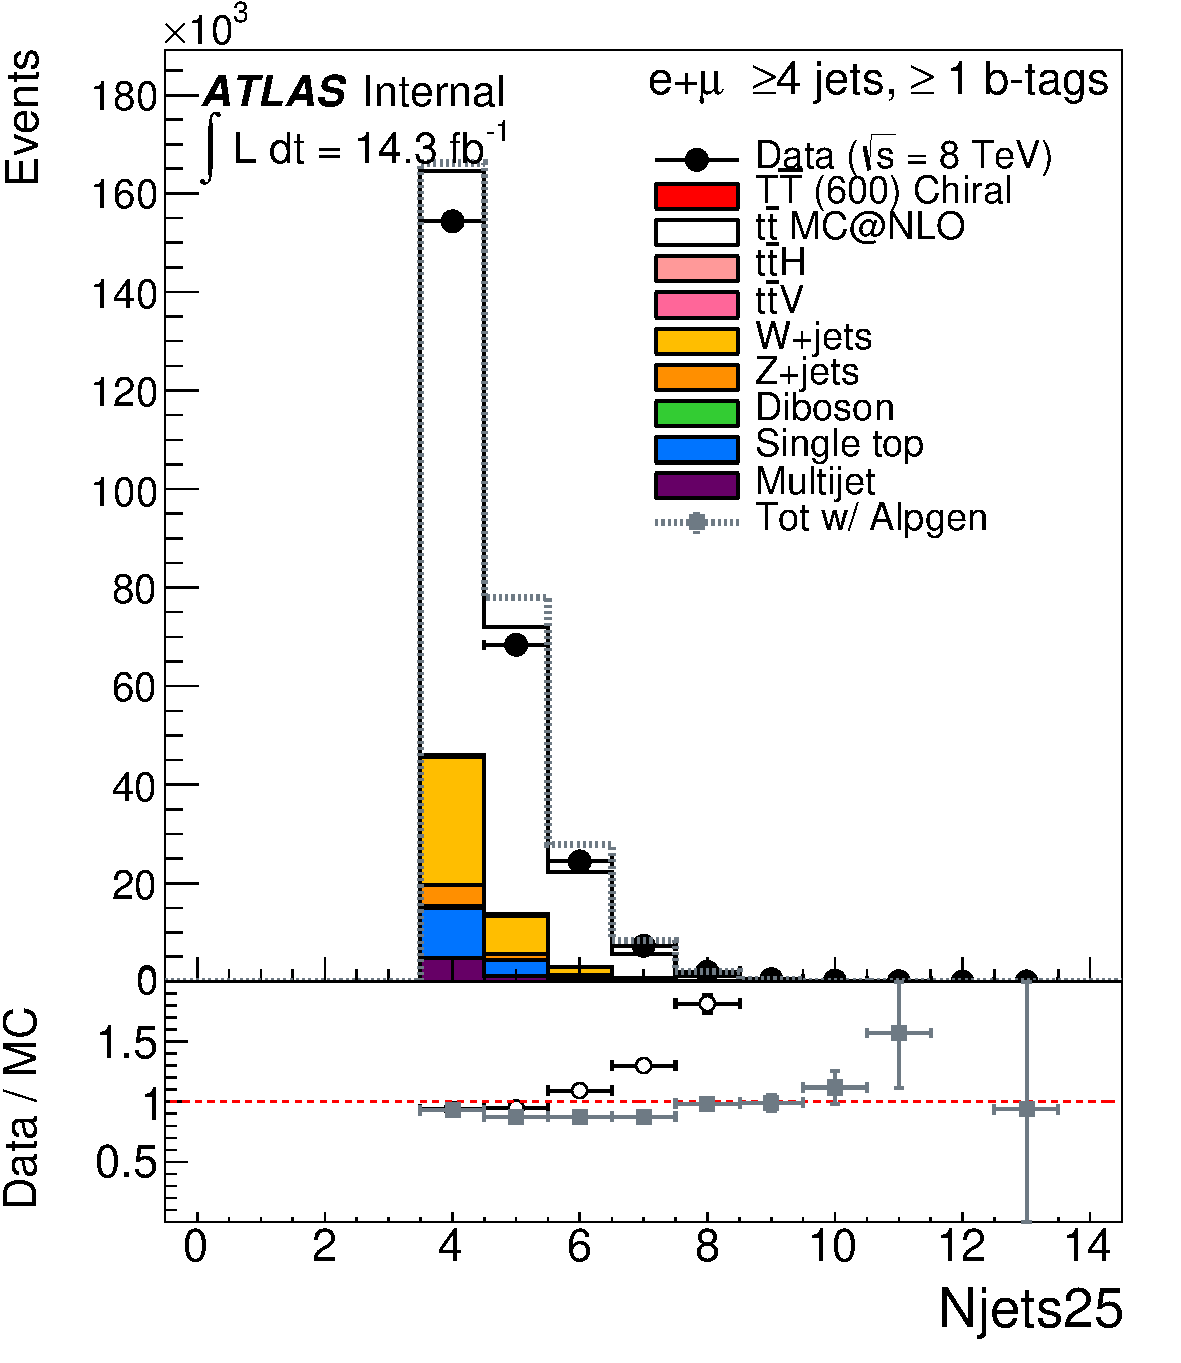
\includegraphics[width=0.32\textwidth]{vlq_analysis/figures/THESIS_c5_presel_noortho_noyields/ELEMUON/4jetin/1btagin/Njets25_ELEMUON_4jetin1btagin_NOMINAL}}
	%\subfigure[]{
  	%\includegraphics[width=0.32\textwidth]{vlq_analysis/figures/THESIS_c5_presel_noortho_noyields/ELEMUON/4jetin/1btagin/JetEta1_ELEMUON_4jetin1btagin_NOMINAL}}\\
	%\subfigure[]{
  	%\includegraphics[width=0.32\textwidth]{vlq_analysis/figures/THESIS_c5_presel_noortho_noyields/ELEMUON/4jetin/1btagin/nWhad_ELEMUON_4jetin1btagin_NOMINAL}}
	%\subfigure[]{
  	%\includegraphics[width=0.32\textwidth]{vlq_analysis/figures/THESIS_c5_presel_noortho_noyields/ELEMUON/4jetin/1btagin/Wlep_MassT_ELEMUON_4jetin1btagin_NOMINAL}}
	%\subfigure[]{
  	%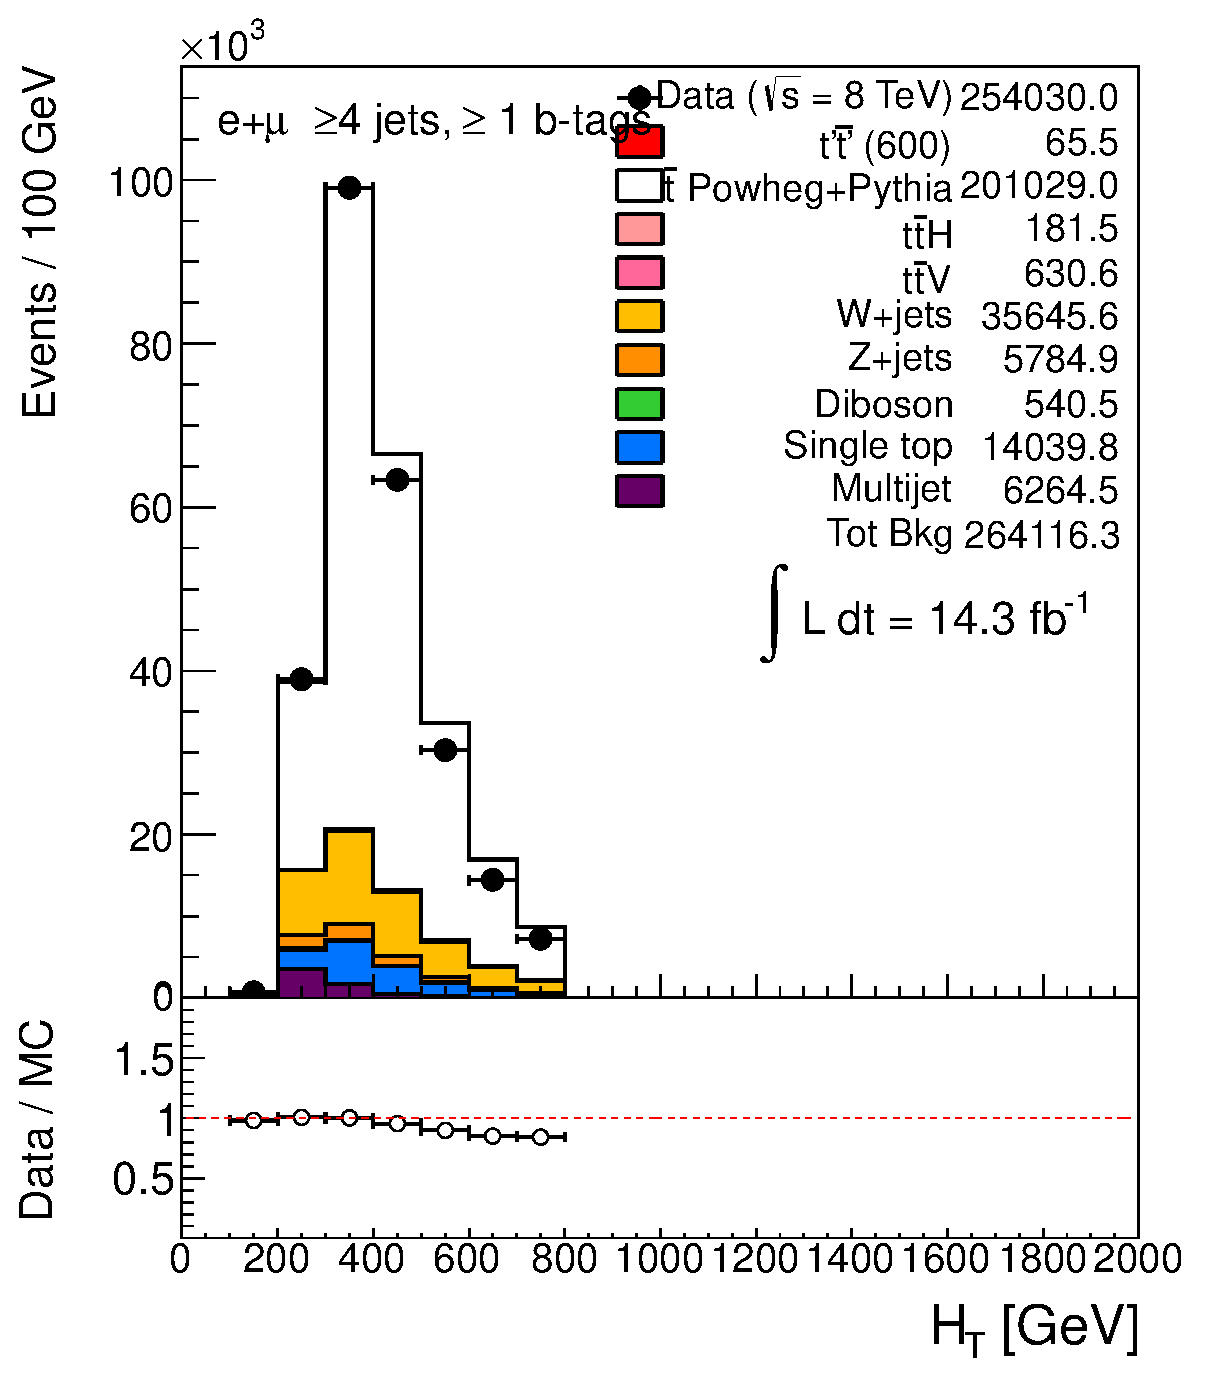
\includegraphics[width=0.32\textwidth]{vlq_analysis/figures/THESIS_c5_presel_noortho_noyields/ELEMUON/4jetin/1btagin/HTAll_ELEMUON_4jetin1btagin_NOMINAL}}
	\caption{Comparison between data and prediction plots for (a) lepton transverse momentum and
        (b) pseudorapidity, (c) missing tranverse energy, (d) transverse mass of $W$ boson, (e)
        leading jet transverse momentum, (f) number of jets with $\pt>25~\gev$.
        The selection is ``preselection'' with a blinding cut to reject signal on
        $\htfj<800\gev$. Systematic uncertainties are not shown.
        \label{fig:ELEMUON_4jetin1btagin}}
\end{center}\end{figure}



\section{Systematic uncertainties}\label{sec:systematics}

In addition to the uncertainty that comes from the stocastical nature
of events we are subject to other sources that are systematical in the sense
that they will bias the result towards a definite direction. They can come from
detector measurements, from the way we reconstruct the objects, from the Monte
Carlo modelling, and can affect either only the normalization of the total event
yield (and are called ``normalization-only'' sytematics) or also the shape 
of the distributions (and are called ``shape and normalization'' systematics).

The individual sources of systematics are treated as uncorrelated, while
the correlations eventually present in the particual systematic uncertainty are 
kept for the various processes and channels. Most of the systematic uncertainties
are common to the two analyses presented with only minor differences, e.g. in the
\htx\  analysis the systematic uncertainty affecting the jet energy scale is
split into 9 components, while it has a unique component in the \wbx\  analysis. 
The full list of systematics considered is presented in 
Table~\ref{tab:SystSummary}, labelling them as  ``normalization-only'' 
or ``shape and normalization'' systematics and indicating the number of components.

\begin{table}[htb]
\centering
\begin{tabular}{lcccc}
\toprule
Systematic uncertainty & \multicolumn{2}{c}{ \wbx\  } & \multicolumn{2}{c}{ \htx\  }\\
 & Status  & Components & Status  & Components\\
\midrule
Luminosity                  &  N & 1 &  N & 1\\
Lepton ID+reco+trigger      &  N & 1 &  N & 1\\
Jet vertex fraction efficiency & SN & 1 & SN & 1\\
Jet energy scale            & SN & 1 & SN & 8\\
Jet energy resolution       & SN & 1 & SN & 1\\
%Jet mass scale               & - & -\\
%Jet mass resolution      & - & -\\
$b$-tagging efficiency      & SN & 9 & SN & 9\\
$c$-tagging efficiency      & SN & 5 & SN & 5\\
Light jet-tagging efficiency    & SN & 1 & SN & 1\\
$t\bar{t}$ cross section    &  N & 1 &  N & 1\\
$t\bar{t}V$ cross section   &  N & 1 &  N & 1\\
$t\bar{t}H$ cross section   & - & - &  N & 1\\
Single top cross section    &  N & 1 &  N & 1\\
Dibosons cross section      &  N & 1 &  N & 1\\
$W$+jets normalization      &  N & 5 &  - & -\\
$Z$+jets normalization      &  N & 1 &  - & -\\
$V$+jets normalization      &  - & - &  N & 1\\
Multijet normalization      &  - & - &  N & 1\\
$t\bar{t}$ modelling        & SN & 3 & SN & 3\\
$V$+jets modelling         & SN & 1 &  - & -\\
$t\bar{t}$+heavy-flavour fractions &  - & -& N & 1\\
%$\TT$ modelling        & - & -\\
\bottomrule
\end{tabular}
\caption{\label{tab:SystSummary} 
List of systematic uncertainties considered in the two analyses. 
We label as ``N'' (``SN'') uncertainties taken as ``normalization-only'' 
(both ``shape'' and ``normalization'')
for all processes and channels. 
Some of the systematic uncertainties are split into more 
components for a more
accurate treatment. }
\end{table}

The systematic uncertainties are treated inside the \mclimit\ 
package~\cite{mclimitATLAS} developed for ATLAS heavy quark
searches based on the original \mclimit\ code developed
by the CDF collaboration~\cite{Heinrich:7587,Junk:8128,Junk:7904}.
Here the  histograms are interpolated between the nominal and the 
systematically shifted templates bin-by-bin, with a shift of $+0.5\sigma$
corresponding to half way between the nominal and the $+1\sigma$ shifted template.
This interpolation method is called vertical morphing and uses a linear 
bin-by-bin interpolation, but for variations below $1\sigma$ we use
quadratic interpolation to ensure a continuous derivative at zero shift.
Pseudoexperiments are generated using these interpolated numbers for
all systematic uncertainties.

Details on specific treatments of systematics in particular channels will
be given in the dedicated sections of the corresponding analysis chapters 
(Section~\ref{sec:wbxSYS} and~\ref{sec:htxSYS}).



\subsection{Luminosity}
\label{sec:syst_lumi}
The uncertainty on the absolute integrated luminosity is estimated to be
of 3.6\%~\cite{lumi}. This systematic uncertainty
is applied to all processes except the QCD multi-jet background.

\subsection{Object definitions}
\label{sec:syst_objects}
The event reconstruction introduces uncertainties on the definition of
leptons, jets and on the $b$-, $c$-, and light flavour-tagging. In the
following the related systematic uncertainties considered are described.

\subsubsection{Lepton reconstruction, identification and trigger scale factors}
\label{sec:syst_lepID}

In Sections~\ref{sec:electrons} and~\ref{sec:muons} the reconstruction
of leptons was introduced, explaining the need of adjusting the
differences between data and simulation in the efficiency for
reconstruction, identification and trigger. This is done by
applying to Monte Carlo samples some scale factors derived 
with tag-and-probe techniques 
on $Z\to \ell^+\ell^-$ ($\ell=e,\mu$) data and simulated samples.
For each of these three sources of systematic uncertainty, 
the overall systematic uncertainty is obtained 
as the quadratic sum of the statistical
and systematic uncertainties on the corresponding scale factor.

In the $e$+jets channel, the systematic uncertainties corresponding to
electron reconstruction, identification and trigger, are 0.3\%, 1.1\% 
and 0.2\%, respectively.
In the $\mu$+jets channel, the systematic uncertainties corresponding to
muon reconstruction, identification and trigger, are 0.2\%, 1.1\% and 1.4\%, 
respectively.
A total uncertainty on the signal and background acceptances of 2\% is estimated.


\subsubsection{Lepton momentum scale and resolution}

To check the accuracy of the lepton momentum scale and resolution
simulated samples of $Z\to \ell^+\ell^-$ and $J/\psi \to \ell^+\ell^-$
are used to reconstruct the particles masses (for electrons also
 $W\to e\nu$ events are used from  $E/p$  studies).
The small discrepancies observed between data and simulation are
corrected adjusting lepton energy scale and resolution in Monte Carlo
samples only for muons, while for electrons energy resolution corrections
are also applied only to Monte Carlo samples but energy scale corrections
are applied to data in all detector regions and to simulation only in 
the calorimeter transition region.
The systematic uncertainties on these scale factors are varied
separately and the result on the total yields are are at the 
sub-percent level and considered therefore ngligible in the analyses.

\subsubsection{JVF efficiency}
\label{sec:syst_jvf}

Recalling the cut applied on the JVF variable (Section~\ref{sec:jets}) 
of $|{\rm JVF}|>0.5$, the per-jet efficiency of this requirement
is estimated in $Z(\to \ell^+\ell^-)$+1-jet events both in data and
Monte Carlo simulation. Event enriched in hard-scatter jets are selected
separately from events enriched in jets from pile-up interactions and
specific efficiency and inefficiency scale factors are measured.
Scale factors for pileup jets are estimated to be consistent with 1, while
efficiency for hard-scatter jets goes from $\sim$1.03 for jets with $\pt=25\gev$
down to $\sim$1.01 for jets with $\pt>150\gev$.
An overall event weight is obtained as the product of all per-jet scale factors
and is applied to the Monte Carlo samples.
The systematic uncertainty from the propagation of the per-jet scale
factor uncertainty gives an overall uncertainty on the signal
and background acceptance of $\sim$2.5\%.


\subsubsection{Jet energy scale}
\label{sec:syst_jes}

The systematic uncertainty on the Jet Energy Scale (JES) 
has been derived combining the information from both test-beam 
and collision data and Monte Carlo
simulation~\cite{ATLASJetEnergyMeasurement, insitu5,insitu6}.  
Pile-up activity produces an additional source of systematic 
uncertainty which depends on the number of primary vertices
and on the average number of interactions per bunch crossing $<\mu>$. 
%The first estimate of the effect of pile-up on the jet energy scale uncertainty was developed in 2011~\cite{insitu6}, and subsequently validated with in situ momentum balance techniques in studies of the 2012 data.
Momentum balance techniques in $Z$+jets, $\gamma$+jets and 
multi-jet events are combined to derive a small residual correction
for jets in the transverse momentum range $20\gev<\pt<\sim1\tev$.

The overall variation due to JES systematic uncertainty 
evaluated in the central detector region 
is $\sim$4\% for jets with $\pt=25\gev$ and improves to $\sim$1\% for  
jets with $\pt=500\gev$~\cite{jesuncertainty}.
The effect of this systematic uncertainty is 
implemented in the analyses by varying in the Monte Carlo samples the 
transverse momentum of all the selected jets by $\pm$1 standard deviation.
In each event the missing transverse momentum \met\ is then corrected consistently to 
the varied $\pt$ of the jets and all the variables involving jets are also
recomputed.

As can be seen in Table~\ref{tab:SystSummary}, for the \htx\ analysis
the JES systematic uncertainty is split into 8
uncorrelated components, each with a different jet $\pt$ and $\eta$
dependence, which are treated independently.
The \wbx\ instead uses the total JES uncertainty as a single uncertainty
resulting from the sum in quadrature of all individual sources.



\subsubsection{Jet energy resolution}
\label{sec:syst_jer}

The Jet Energy Resolution (JER) was measured 
with two {\em in-situ} techniques~\cite{ATLASJetEnergyMeasurement}
as a function of the jet transverse momentum and pseudo-rapidity.
It is consistent in data and Monte Carlo simulation and no corrections
are needed.
To account for the systematic uncertainty the quadratic difference 
between the JER in data and in simulated samples is used
to smear the energy of jets in Monte Carlo simulation and a new
varied sample is obtained with a different normalisation and 
variable distributions shapes. The final result is then symmetrised
to obtain both positive and negative variations.
%In order to propagate the uncertainty in the $\pt$ resolution, for each jet in the simulation, a random number $r$ is drawn from a Gaussian distribution with mean 0 and sigma equal to the difference in quadrature between the fractional $\pt$ resolution with the tool and the nominal one.  The jet 4-momentum is then scaled by a factor $1+r$. This jet energy resolution uncertainty is assumed to be fully correlated point-by-point.
%The same rebinning algorithm as discussed in Section~\ref{sec:syst_jes} is applied.


\subsubsection{Heavy- and light-flavour tagging}
\label{sec:syst_btag}


The efficiencies in heavy flavour ($b$ and $c$) jets identification with
the $b$-tagging algorithm are measured in data and depend on the individual
jet flavour~\cite{BTaggingEfficiency,CTaggingEfficiency,LightTaggingEfficiency}.
These efficiencies are measured from data and depend on the jet flavour:
in Monte Carlo events $b$ ($c$) jet efficiencies are corrected with scale factors
of 0.9--1.0 (1.1--1.2) depending on $\pt$, light jet efficiencies are corrected 
with a  scale factor of $\sim$1.3.
Every jet in the Monte Carlo simulated events is corrected depending
on its flavour, $\pt$ and $\eta$
The uncertainty on these scale factors is 
between 7\% and 13\% for $b$ jets, between 15\% and 39\% for $c$ jets,
and $\sim$25\% for light jets.

As was reported in Table~\ref{tab:SystSummary}, the systematic uncertainty
on \btag ging (\ctag ging) efficiency is divided into nine (five) independent 
components that correspond to an eigenvector from the diagonalization of the
matrix containing the information on the total uncertainty 
per $\pt$ bin and the bin-to-bin correlations (see~\cite[Appendix P]{VHbb} for
more details).
These individual sources of systematic uncertainties 
are taken as uncorrelated between $b$, $c$ jets, and
light flavour jets. In Monte Carlo simulated events 
a per-jet weighting procedure~\cite{IFAEBtagNote}
is applied in order to propagate the \btag ging calibration
and related uncertainties.

\subsection{Theoretical cross-sections}
\label{sec:syst_bkgxsect}

Normalization-only systematic uncertainties on the theoretical
cross-sections are considered as follows:
+10\%/-11\% for the inclusive $t\bar{t}$
production cross section evaluated at approximate NNLO using 
\texttt{HATHOR}~\cite{ttbarxs}; +5\%/-4\% and $\pm 5\%$ 
for the theoretical cross sections of the single
top~\cite{stopxs,stopxs_2} and diboson~\cite{dibosonxs} backgrounds
respectively; +12\%/-17\% and  $\pm 30\%$ 
for the theoretical cross sections of the $t\bar{t}H$~\cite{lhcxs} and 
$t\bar{t}V$~\cite{ttbarVxs1,ttbarVxs2} backgrounds respectively.


\subsection{Normalizations of data-driven backgrounds and background modeling}
\label{sec:syst_norm}

Because of the differences between the effects of these systematic uncertainties
in the \wbx\ and \htx\ analyses, the reader is referred to the specific 
Sections~\ref{sec:wbxSYS} and~\ref{sec:htxSYS}


%
\section{Search for \TTbar\ pairs decaying to $Wb+X$}\label{sec:wbx}

\subsection{Boosted $W$ reconstruction}\label{subsec:boostedW}

\subsection{Control regions}\label{sec:wbxCR}

\subsection{Event selection}\label{sec:wbxEVT}

%\subsection{}\label{sec:}

%\subsection{}\label{sec:}

\subsection{Systematics}\label{sec:wbxSYS}

%
\section{Preliminary search for \TTbar\ pairs decaying to $Ht+X$}\label{sec:htx}

\subsection{Control regions}\label{sec:htxCR}

\subsection{Event selection}\label{sec:htxEVT}

%\subsection{}\label{sec:}

%\subsection{}\label{sec:}

\subsection{Systematics}\label{sec:htxSYS}



\section{Statistical analysis}\label{sec:cls}

To test the presence or absence of signals from new physics we use the
\cls{s}\ method~\cite{cls,cls_2} originally developed in the context of Higgs
searches at the LEP collider~\cite{Read:451614}.
The fundamental principle of this technique is that, in order to 
exclude or verify a theory predicting some kind of signal over some other kind
of background, both ``background only'' and ``signal plus background''
hypotheses have to be tested. Once a test statistic $Q$ has been chosen
analysis-wise, two confidence levels (CL) are defined for the two hypotheses:
\begin{eqnarray}\label{eq:clbclsb}
\cls{b} &=& P(Q \leq Q_{\rm obs}|\mathcal{H}_{b}),\\
\cls{s+b} &=& P(Q \leq Q_{\rm obs}|\mathcal{H}_{s+b}),
\end{eqnarray}
with $Q_{\rm obs}$ being the observed value in data of the 
test statistic. It is good to identify well separated test statistic
distributions in order to be able to clearly distinguish between 
events consistent with the backgroud only prediction and events
showing deviations consistent with the signal+background hypothesis.

The \cls{s}\ is then defined as the ratio of the two:
\begin{equation}\label{eq:cls}
\cls{s} = \cls{s+b}/\cls{b}
\end{equation}
and its meaning is given by its relation with the confidence 
level $CL$ for the exclusion of the signal hypothesis 
$(1 - \cls{s}) \leq CL$.
%i.e. values of $\cls{s}<0.05$ 
Similarly, the confidence level for excluding the background only
hypothesis is the $p$-value $1 - \cls{b}$ and the value required to claim 
discovery is of $\sim 10^{-7}$. The motivation that led to
the definition of \cls{s} instead of using \cls{s+b}, which also
corresponds to the confidence level in excluding the signal+background
hypothesis, is that the latter might wrongly exclude scenarios to
which the analysis is simply not sensitive to like is the general case
for searches for rare events.

\begin{figure}[htb]\begin{center}
        \psfrag{AAA}{\tiny $P(f(Q)|\mathcal{H}_{b})$}
        \psfrag{BBB}{\tiny $P(f(Q)|\mathcal{H}_{s+b})$}
        \psfrag{CCC}{\tiny $1 - CL_{b}$}
        \psfrag{DDD}{\tiny $CL_{s+b}$}
        \psfrag{XXX}{$f(Q)$}
        \psfrag{YYY}{\hskip-10ex Probability density}
	\subfigure[]{\label{fig:sepLLR}
  	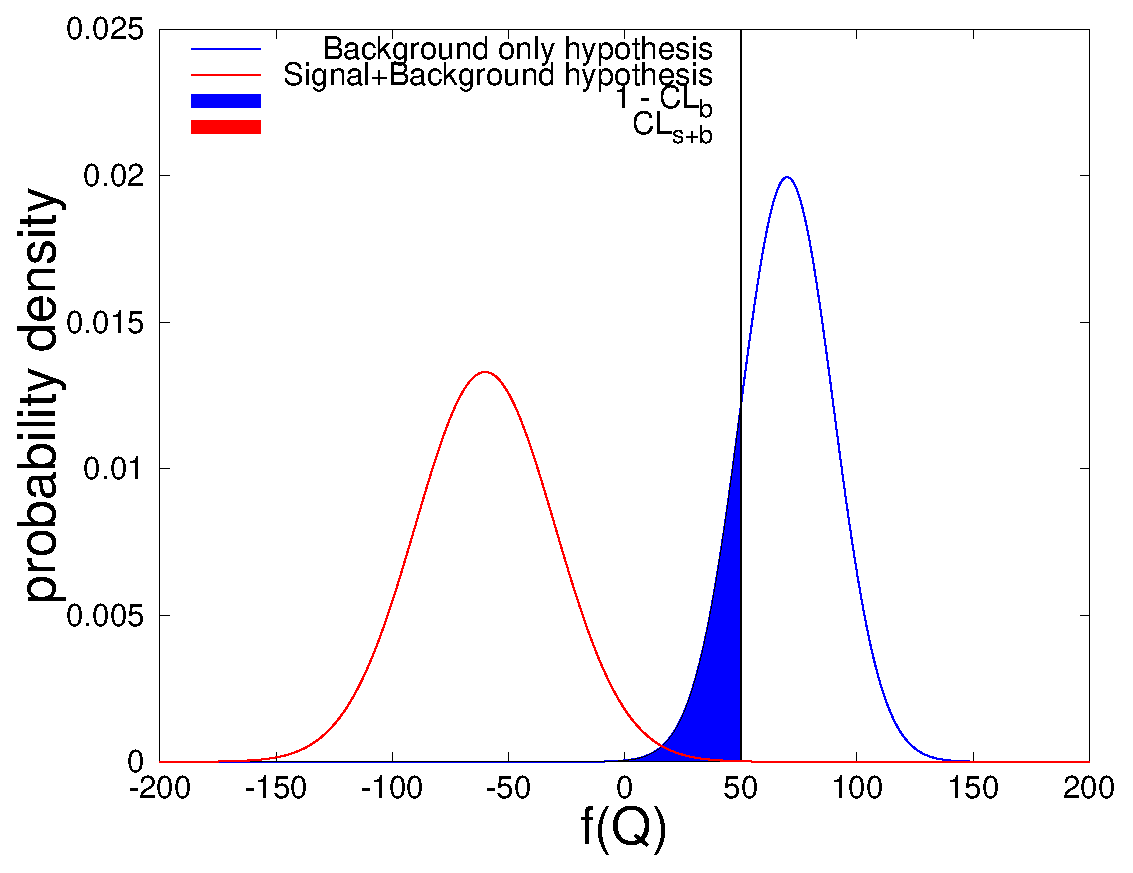
\includegraphics[width=0.45\textwidth]{vlq_analysis/figures/separatedLLR}}
	\subfigure[]{\label{fig:ovrLLR}
  	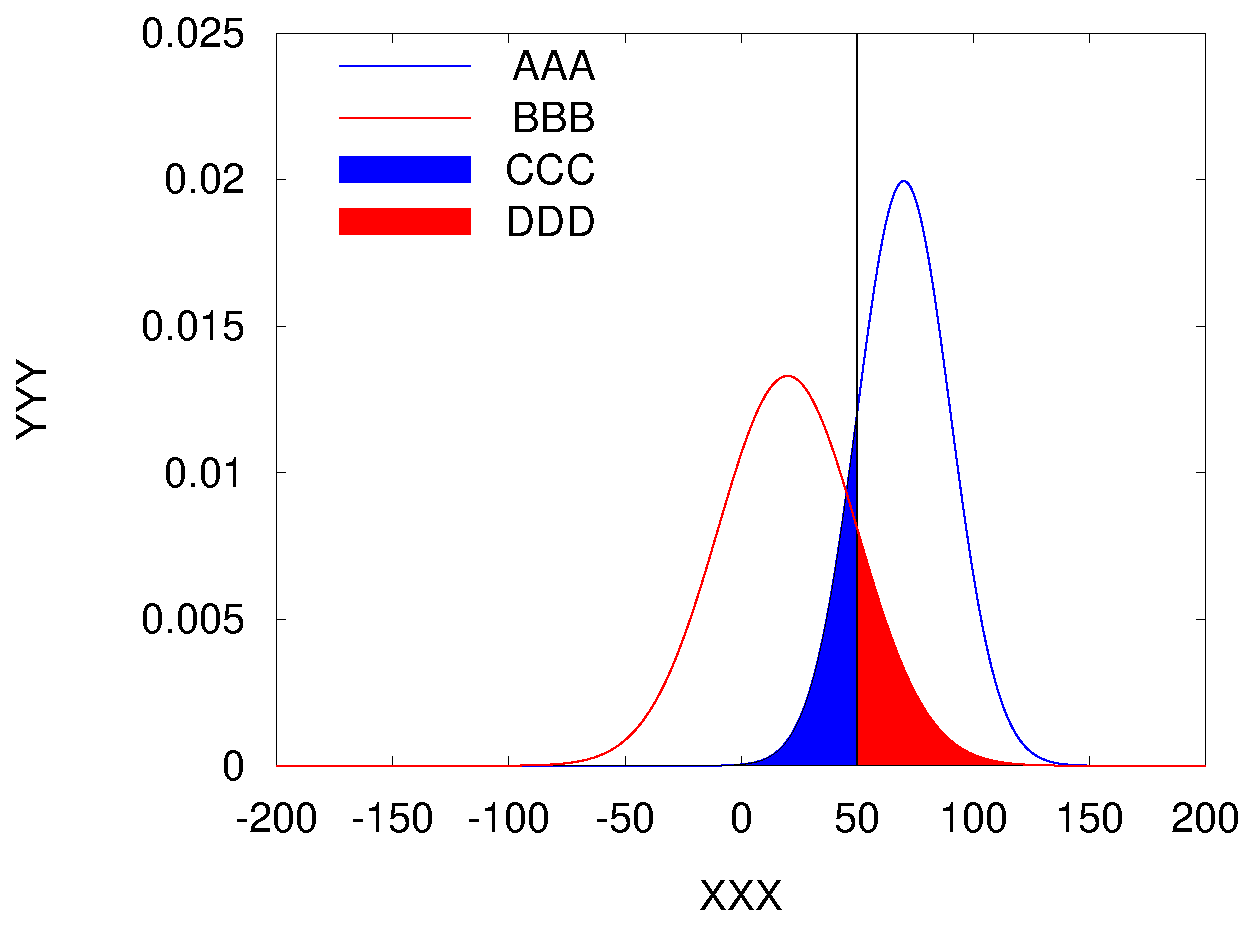
\includegraphics[width=0.45\textwidth]{vlq_analysis/figures/overlappedLLR}}
	\caption{Example of (a) sensitive and (b) not sensitive analyses using the test 
        statistics $f(Q)$, often chosen as $-2\log Q$.}
\end{center}\end{figure}


For the two analyses presented in this dissertation, the test statistic
is defined as a log-likelihood ratio 
\begin{equation}\label{eq:llr}
LLR = -2\log \dfrac{\mathcal{L}({\rm data}|\mathcal{H}_{s+b})}{\mathcal{L}({\rm data}|\mathcal{H}_{b})},
\end{equation}
where the likelihoods $\mathcal{L}({\rm data}|\mathcal{H}_{s+b})$
 and $\mathcal{L}({\rm data}|\mathcal{H}_{b})$ for 
signal+background and background only hypothesis
are built from the chosen discriminant variable distribution 
as the bin by bin product of Poisson probabilities to observe the
data under one or the other hypothesis.
Eventually more than one channel can be combined (like will be
the case in the \htx\ analysis) and the complete formula for
the likelihood computation reads:
\begin{align}
-2 \log {\cal L}({\rm data}|\mathcal{H}_x) 
   & =  
   %=
   -2 \log {\cal L}(\vec{n}|R,\vec{s},\vec{b},\vec{\theta}) \notag\\
   %=
   & =  
  -2 \sum_{i=1}^{N_{chan}}\sum_{j=1}^{N_{bins}} (n_{ij}\log \mu_{ij}-\mu_{ij})+\sum_{k=1}^{N_{par}} \theta_k^2.
\end{align}
Here the first sum is over the number of channels
combined in the analysis $N_{chan}\geq 1$ and the 
second sum is over the number of the discriminant variable
histogram bins $N_{bins}$. $n_{ij}$ ($\mu_{ij}$) is the 
number of events in data (expected number of events) 
for channel $i$ and histogram bin $j$. $\mu_{ij}$ is given by
$\mu_{ij} = R s_{ij}(\vec{\theta})+ b_{ij}(\vec{\theta})$, 
where $s_{ij}$  and $b_{ij}$ represent the
expected signal and background yields, 
the first being equal to zero in the background only hypothesis.
$R$ is a scaling 
parameter applied to the signal
to test the sensitivity of the search and $\vec{\theta}$
are the nuisance parameters parametrizing the effect of
systematic uncertainties. 
The statistical uncertainty of the Monte Carlo samples is 
also taken into account when computing our likelihoods as
an uncertainty of the templates, which in the case of
the non-$t\bar{t}$ background are merged into a single
template  with different weights.
%The {\sc mclimit} flag used is 2, meaning we consider the uncertainties as given by the uncertainties of the templates. 
%This allows us to correctly estimate the statistical uncertainty when many templates are merged together with different weights, such as in the case of the merged non-$t\bar{t}$ background.
%These parameters are assigned Gaussian penalty terms in the likelihood corresponding
%to their nominal uncertainties.
For both hypotheses pseudoexperiments are generated to
account in each bin for statistical fluctuations (Poisson-distributed)
and systematic variations (Gaussian-distributed). The effect of
systematic uncertainties are described by nuisance parameters taken
at their nominal values and no parameter fitting is performed.
In the case of the \htx\ analysis it will be explained that
two additional nuisance parameters are introduced and fitted
to help costraining the sensitivity degradation due to a poor
Monte Carlo modeling of \ttbar\ heavy flavor component.

In absence of data excess over background prediction, values of
$\cls{s}<0.05$ are considered to exclude a signal cross section
at 95\% CL.



\clearpage{\pagestyle{empty}\cleardoublepage}
\clearpage{\pagestyle{empty}\cleardoublepage}

\chapter{Statistical treatment and Results}\label{chap:results}



\section{The CL$_s$ method}\label{sec:cls}


\section{Systematics}\label{sec:systematics}


\section{Results}\label{sec:results}


\clearpage{\pagestyle{empty}\cleardoublepage}

\phantomsection
\addcontentsline{toc}{chapter}{Conclusions}
\clearpage{\pagestyle{empty}\cleardoublepage}

\chapter*{Conclusions and outlook}\label{chap:conclusions}

\vskip-1.5cm

Two quasi-model independent searches for 
pair production of vector-like top partners 
in proton-proton collisions at a \cme\ of 8~\tev\ 
have been presented in this dissertation. The final states considered
for both analyses involve one lepton and many jets but different
strategies are adopted in order to achieve sensitivities in different
corners of the decay phase space. Indeed, a peculiar fact for these
searches that has been stressed many times over these pages is the 
unpredicted nature of the heavy vector-like top partners model. 
As a direct consequence, the two analyses have been designed
and developed to be optimized for a particular decay mode and
to have orthogonal channels in order to allow
for a combined search that could exploit the specific sensitivities.

Three particular models, interesting from a theoretical point
of view (but not for this more favoured than others), are considered
over the two analyses: the chiral fourth-generation, with 
BR$(T\to Wb)=1$ for any value of the heavy quark mass; 
the singlet vector-like, with BR$(T\to Wb)\sim 0.5$ and 
BR$(T\to Ht)\sim 0.3$ for almost all
values of the heavy quark mass considered in the searches;
the doublet vector-like, with BR$(T\to Wb)= 0$ and 
BR$(T\to Ht)\in$ [0.50, 0.75] for all the values of the heavy quark mass.
In the \wbx\ analysis, it was possible to exclude at a 95\% CL
pair-produced chiral fourth-generation top partners and vector-like
$Y$ quarks with masses up to 740~\gev, and pair-produced vector-like 
singlet top partners with  masses up to 505~\gev.
In the \htx\ analysis, it was possible to exclude at a 95\% CL
pair-produced vector-like singlet and doublet top partners with 
masses up to 640~\gev\ and 790~\gev\ respectively.
When the two analyses are combined, the observed exclusion limit
for the only model where both analyses are sensitive, the
vector-like singlet $T$, is pushed $\sim$30~\gev\ further the
best result of the two, obtained by the \htx\ analysis,
achieving a 95\% CL exclusion of pair-produced vector-like singlet 
top partners with masses up to 670~\gev. While this might not
look like a significant improvement, the power of the combination
of the two searches is evident looking at the coverage of the
two-dimensional branching ratio plane, where  95\% CL exclusion is set for
pair-produced vector-like top partners with masses up to 550~\gev\ 
independently from the model, and also the plane for the 600~\gev\ mass
point is almost fully excluded. This strongly encourages to perform,
in the future, full combination of searches for vector-like quarks.

The mass range excluded at 95\% CL up to now
is getting closer and closer to the point where pair-production
of vector-like quarks will start to be disfavoured with respect
to single production. In this sense, while it is desirable to continue to
exploit the experience achieved up to now with the searches for
pair-produced vector-like quarks in the single lepton and multi-lepton
channels, it is a good idea to start designing searches for
single-produced vector-like quarks for LHC Phase-II.
Further improvements are possible for the searches
presented in this dissertation without changing the core of
the analysis strategies. During Phase-II they will benefit
of the increased \cme\ available for heavy quark production
in pp collisions with \rts=14~\tev\ and of the high integrated
luminosity (100~\ifb\ of data are expected over three years
of operation). With high luminosity comes the challenge of
dealing with higher pile-up, but considering that vector-like
quark searches involve high-\pt\ objects this should not
represent a major issue.

Besides the great discovery potential, the combination
of multiple searches will provide useful insights on the
exotic quark properties, like their quantum numbers or
the measurement of their branching ratios. 
Adding searches for single production of vector-like quarks
would also allow to measure the electroweak couplings of
these particles with the Standard Model quarks from the third generation.
Finally, these searches are even more interesting since
they will probe a wide range of
signatures that are often shared with other new physics
scenarios. Given the fact that during these last successful years
of LHC operation no hints on what lies ``beyond the Standard Model''
have emerged, the winning strategy is for sure not to confine ourselves 
to exclusive models.


\clearpage{\pagestyle{empty}\cleardoublepage}

\appendix

\clearpage{\pagestyle{empty}\cleardoublepage}

\chapter{}\label{app:}


\clearpage{\pagestyle{empty}\cleardoublepage}

\clearpage{\pagestyle{empty}\cleardoublepage}

\chapter{}\label{app:}


\clearpage{\pagestyle{empty}\cleardoublepage}
\clearpage{\pagestyle{empty}\cleardoublepage}

\chapter{Search for $T\bar{T}\to Wb+X$ at $\sqrt{7}~$\tev}\label{chap:wbx7tev}


%\clearpage{\pagestyle{empty}\cleardoublepage}
%\clearpage{\pagestyle{empty}\cleardoublepage}

\chapter{Preliminary search  for \TTbar\ pairs decaying to $Ht+X$}\label{chap:htx}

\section{Control regions}\label{sec:htxCR}

\section{Event selection}\label{sec:htxEVT}

%\section{}\label{sec:}

%\section{}\label{sec:}

\section{Systematics}\label{sec:htxSYS}



%%%%NB COPY PASTE
The total prior systematic uncertainty
in the background normalisation in the $\geq 4$ $b$-tags channel is 
$\sim$42\%, with the dominant uncertainties being from $b$ tagging efficiency (16\%),
$c$ tagging efficiency (11\%), jet energy scale (11\%), $t\bar{t}$ modelling (11\%), 
$t\bar{t}$+heavy-flavour fractions (32\%) and $t\bar{t}$ cross section (10\%).
As a result of the two-parameter fit, the total background uncertainty is reduced 
by about 80\% in this channel. The total  systematic uncertainty
in the signal normalisation in the $\geq 4$ $b$-tags channel is 
$\sim$21\%, completely dominated by the uncertainty in the $b$ tagging efficiency.


%\phantomsection
%\addcontentsline{toc}{chapter}{Ringraziamenti}
%\input{smallstuff/ringraziamenti}

\clearpage{\pagestyle{empty}\cleardoublepage}


\backmatter

%\nocite{}
\phantomsection
\addcontentsline{toc}{chapter}{Bibliography}

%\bibliographystyle{woc}
\bibliographystyle{unsrt}
\bibliography{bibliography/biblio}

\clearpage{\pagestyle{empty}\cleardoublepage}



\end{document}
